
\documentclass[11pt]{article}
\usepackage[utf8]{inputenc} % Required for inputting international characters
\usepackage[T1]{fontenc} % Output font encoding for international characters
\usepackage{caption} % for table captions
\usepackage{amsmath} % for multi-line equations and piecewises
\DeclareMathOperator{\sign}{sign}
\usepackage{graphicx}
\usepackage{relsize}
\usepackage{xspace}
\usepackage{verbatim} % for block comments
\usepackage{subcaption} % for subfigures
\usepackage{enumitem} % for a) b) c) lists
\newcommand{\Cyclus}{\textsc{Cyclus}\xspace}%
\newcommand{\Cycamore}{\textsc{Cycamore}\xspace}%
\newcommand{\deploy}{\texttt{d3ploy}\xspace}%
\newcommand{\Deploy}{\texttt{D3ploy}\xspace}%
\usepackage{tabularx}
\usepackage{color}
\usepackage{multirow}
\usepackage[acronym,toc]{glossaries}
\newacronym[longplural={metric tons of heavy metal}]{MTHM}{MTHM}{metric ton of heavy metal}
\newacronym{ABM}{ABM}{agent-based modeling}
\newacronym{ACDIS}{ACDIS}{Program in Arms Control \& Domestic and International Security}
\newacronym{AHTR}{AHTR}{Advanced High Temperature Reactor}
\newacronym{ANDRA}{ANDRA}{Agence Nationale pour la gestion des D\'echets RAdioactifs, the French National Agency for Radioactive Waste Management}
\newacronym{ANL}{ANL}{Argonne National Laboratory}
\newacronym{API}{API}{application programming interface}
\newacronym{ARCH}{ARCH}{autoregressive conditional heteroskedastic}
\newacronym{ARE}{ARE}{Aircraft Reactor Experiment}
\newacronym{ARFC}{ARFC}{Advanced Reactors and Fuel Cycles}
\newacronym{ARMA}{ARMA}{autoregressive moving average}
\newacronym{ASME}{ASME}{American Society of Mechanical Engineers}
\newacronym{ATWS}{ATWS}{Anticipated Transient Without Scram}
\newacronym{BDBE}{BDBE}{Beyond Design Basis Event}
\newacronym{BIDS}{BIDS}{Berkeley Institute for Data Science}
\newacronym{BOL}{BOL}{Beginning-of-Life}
\newacronym{BSD}{BSD}{Berkeley Software Distribution}
\newacronym{CAFCA}{CAFCA}{ Code for Advanced Fuel Cycles Assessment }
\newacronym{CASL}{CASL}{Consortium for Advanced Simulation of Light Water Reactors}
\newacronym{CDTN}{CDTN}{Centro de Desenvolvimento da Tecnologia Nuclear}
\newacronym{CEA}{CEA}{Commissariat \`a l'\'Energie Atomique et aux \'Energies Alternatives}
\newacronym{CI}{CI}{continuous integration}
\newacronym{CNEC}{CNEC}{Consortium for Nonproliferation Enabling Capabilities}
\newacronym{CNEN}{CNEN}{Comiss\~{a}o Nacional de Energia Nuclear}
\newacronym{CNERG}{CNERG}{Computational Nuclear Engineering Research Group}
\newacronym{COSI}{COSI}{Commelini-Sicard}
\newacronym{COTS}{COTS}{commercial, off-the-shelf}
\newacronym{CSNF}{CSNF}{commercial spent nuclear fuel}
\newacronym{CTAH}{CTAHs}{Coiled Tube Air Heaters}
\newacronym{CUBIT}{CUBIT}{CUBIT Geometry and Mesh Generation Toolkit}
\newacronym{CURIE}{CURIE}{Centralized Used Fuel Resource for Information Exchange}
\newacronym{DAG}{DAG}{directed acyclic graph}
\newacronym{DANESS}{DANESS}{Dynamic Analysis of Nuclear Energy System Strategies}
\newacronym{DBE}{DBE}{Design Basis Event}
\newacronym{DESAE}{DESAE}{Dynamic Analysis of Nuclear Energy Systems Strategies}
\newacronym{DHS}{DHS}{Department of Homeland Security}
\newacronym{DOE}{DOE}{Department of Energy}
\newacronym{DRACS}{DRACS}{Direct Reactor Auxiliary Cooling System}
\newacronym{DRE}{DRE}{dynamic resource exchange}
\newacronym{DSNF}{DSNF}{DOE spent nuclear fuel}
\newacronym{DYMOND}{DYMOND}{Dynamic Model of Nuclear Development }
\newacronym{EBS}{EBS}{Engineered Barrier System}
\newacronym{EDZ}{EDZ}{Excavation Disturbed Zone}
\newacronym{EIA}{EIA}{U.S. Energy Information Administration}
\newacronym{EPA}{EPA}{Environmental Protection Agency}
\newacronym{EP}{EP}{Engineering Physics}
\newacronym{FCO}{FCO}{Fuel Cycle Options}
\newacronym{FCT}{FCT}{Fuel Cycle Technology}
\newacronym{FCWMD}{FCWMD}{Fuel Cycle and Waste Management Division}
\newacronym{FEHM}{FEHM}{Finite Element Heat and Mass Transfer}
\newacronym{FEPs}{FEPs}{Features, Events, and Processes}
\newacronym{FHR}{FHR}{Fluoride-Salt-Cooled High-Temperature Reactor}
\newacronym{FLiBe}{FLiBe}{Fluoride-Lithium-Beryllium}
\newacronym{GCAM}{GCAM}{Global Change Assessment Model}
\newacronym{GDSE}{GDSE}{Generic Disposal System Environment}
\newacronym{GDSM}{GDSM}{Generic Disposal System Model}
\newacronym{GENIUSv1}{GENIUSv1}{Global Evaluation of Nuclear Infrastructure Utilization Scenarios, Version 1}
\newacronym{GENIUSv2}{GENIUSv2}{Global Evaluation of Nuclear Infrastructure Utilization Scenarios, Version 2}
\newacronym{GENIUS}{GENIUS}{Global Evaluation of Nuclear Infrastructure Utilization Scenarios}
\newacronym{GPAM}{GPAM}{Generic Performance Assessment Model}
\newacronym{GRSAC}{GRSAC}{Graphite Reactor Severe Accident Code}
\newacronym{GUI}{GUI}{graphical user interface}
\newacronym{HLW}{HLW}{high level waste}
\newacronym{HPC}{HPC}{high-performance computing}
\newacronym{HTC}{HTC}{high-throughput computing}
\newacronym{HTGR}{HTGR}{High Temperature Gas-Cooled Reactor}
\newacronym{IAEA}{IAEA}{International Atomic Energy Agency}
\newacronym{IEMA}{IEMA}{Illinois Emergency Mangament Agency}
\newacronym{INL}{INL}{Idaho National Laboratory}
\newacronym{IPRR1}{IRP-R1}{Instituto de Pesquisas Radioativas Reator 1}
\newacronym{IRP}{IRP}{Integrated Research Project}
\newacronym{ISFSI}{ISFSI}{Independent Spent Fuel Storage Installation}
\newacronym{ISRG}{ISRG}{Independent Student Research Group}
\newacronym{JFNK}{JFNK}{Jacobian-Free Newton Krylov}
\newacronym{LANL}{LANL}{Los Alamos National Laboratory}
\newacronym{LBNL}{LBNL}{Lawrence Berkeley National Laboratory}
\newacronym{LCOE}{LCOE}{levelized cost of electricity}
\newacronym{LDRD}{LDRD}{laboratory directed research and development}
\newacronym{LFR}{LFR}{Lead-Cooled Fast Reactor}
\newacronym{LGPL}{LGPL}{Lesser GNU Public License}
\newacronym{LLNL}{LLNL}{Lawrence Livermore National Laboratory}
\newacronym{LMFBR}{LMFBR}{Liquid-Metal-cooled Fast Breeder Reactor}
\newacronym{LOFC}{LOFC}{Loss of Forced Cooling}
\newacronym{LOHS}{LOHS}{Loss of Heat Sink}
\newacronym{LOLA}{LOLA}{Loss of Large Area}
\newacronym{LP}{LP}{linear program}
\newacronym{LWR}{LWR}{Light Water Reactor}
\newacronym{MARKAL}{MARKAL}{MARKet and ALlocation}
\newacronym{MA}{MA}{minor actinide}
\newacronym{MCNP}{MCNP}{Monte Carlo N-Particle code}
\newacronym{MILP}{MILP}{mixed-integer linear program}
\newacronym{MIT}{MIT}{the Massachusetts Institute of Technology}
\newacronym{MOAB}{MOAB}{Mesh-Oriented datABase}
\newacronym{MOOSE}{MOOSE}{Multiphysics Object-Oriented Simulation Environment}
\newacronym{MOX}{MOX}{mixed oxide}
\newacronym{MSBR}{MSBR}{Molten Salt Breeder Reactor}
\newacronym{MSRE}{MSRE}{Molten Salt Reactor Experiment}
\newacronym{MSR}{MSR}{Molten Salt Reactor}
\newacronym{NAGRA}{NAGRA}{National Cooperative for the Disposal of Radioactive Waste}
\newacronym{NCSA}{NCSA}{National Center for Supercomputing Applications}
\newacronym{NEAMS}{NEAMS}{Nuclear Engineering Advanced Modeling and Simulation}
\newacronym{NEUP}{NEUP}{Nuclear Energy University Programs}
\newacronym{NFCSim}{NFCSim}{Nuclear Fuel Cycle Simulator}
\newacronym{NFC}{NFC}{Nuclear Fuel Cycle}
\newacronym{NGNP}{NGNP}{Next Generation Nuclear Plant}
\newacronym{NMWPC}{NMWPC}{Nuclear MW Per Capita}
\newacronym{NNSA}{NNSA}{National Nuclear Security Administration}
\newacronym{NPRE}{NPRE}{Department of Nuclear, Plasma, and Radiological Engineering}
\newacronym{NQA1}{NQA-1}{Nuclear Quality Assurance - 1}
\newacronym{NRC}{NRC}{Nuclear Regulatory Commission}
\newacronym{NSF}{NSF}{National Science Foundation}
\newacronym{NSSC}{NSSC}{Nuclear Science and Security Consortium}
\newacronym{NUWASTE}{NUWASTE}{Nuclear Waste Assessment System for Technical Evaluation}
\newacronym{NWF}{NWF}{Nuclear Waste Fund}
\newacronym{NWTRB}{NWTRB}{Nuclear Waste Technical Review Board}
\newacronym{OCRWM}{OCRWM}{Office of Civilian Radioactive Waste Management}
\newacronym{ORION}{ORION}{ORION}
\newacronym{ORNL}{ORNL}{Oak Ridge National Laboratory}
\newacronym{PARCS}{PARCS}{Purdue Advanced Reactor Core Simulator}
\newacronym{PBAHTR}{PB-AHTR}{Pebble Bed Advanced High Temperature Reactor}
\newacronym{PBFHR}{PB-FHR}{Pebble-Bed Fluoride-Salt-Cooled High-Temperature Reactor}
\newacronym{PEI}{PEI}{Peak Environmental Impact}
\newacronym{PH}{PRONGHORN}{PRONGHORN}
\newacronym{PI}{PI}{Principal Investigator}
\newacronym{PNNL}{PNNL}{Pacific Northwest National Laboratory}
\newacronym{PRIS}{PRIS}{Power Reactor Information System}
\newacronym{PRKE}{PRKE}{Point Reactor Kinetics Equations}
\newacronym{PSPG}{PSPG}{Pressure-Stabilizing/Petrov-Galerkin}
\newacronym{PWAR}{PWAR}{Pratt and Whitney Aircraft Reactor}
\newacronym{PWR}{PWR}{Pressurized Water Reactor}
\newacronym{PyNE}{PyNE}{Python toolkit for Nuclear Engineering}
\newacronym{PyRK}{PyRK}{Python for Reactor Kinetics}
\newacronym{QA}{QA}{quality assurance}
\newacronym{RDD}{RD\&D}{Research Development and Demonstration}
\newacronym{RD}{R\&D}{Research and Development}
\newacronym{RELAP}{RELAP}{Reactor Excursion and Leak Analysis Program}
\newacronym{RIA}{RIA}{Reactivity Insertion Accident}
\newacronym{RIF}{RIF}{Region-Institution-Facility}
\newacronym{SAM}{SAM}{Simulation and Modeling}
\newacronym{SCF}{SCF}{Software Carpentry Foundation}
\newacronym{SFR}{SFR}{Sodium-Cooled Fast Reactor}
\newacronym{SINDAG}{SINDA{\textbackslash}G}{Systems Improved Numerical Differencing Analyzer $\backslash$ Gaski}
\newacronym{SKB}{SKB}{Svensk K\"{a}rnbr\"{a}nslehantering AB}
\newacronym{SNF}{SNF}{spent nuclear fuel}
\newacronym{SNL}{SNL}{Sandia National Laboratory}
\newacronym{SNM}{SNM}{Special Nuclear Material}
\newacronym{STC}{STC}{specific temperature change}
\newacronym{SUPG}{SUPG}{Streamline-Upwind/Petrov-Galerkin}
\newacronym{SWF}{SWF}{Separations and Waste Forms}
\newacronym{SWU}{SWU}{Separative Work Unit}
\newacronym{SandO}{S\&O}{Signatures and Observables}
\newacronym{THW}{THW}{The Hacker Within}
\newacronym{TRIGA}{TRIGA}{Training Research Isotope General Atomic}
\newacronym{TRISO}{TRISO}{Tristructural Isotropic}
\newacronym{TSM}{TSM}{Total System Model}
\newacronym{TSPA}{TSPA}{Total System Performance Assessment for the Yucca Mountain License Application}
\newacronym{UDB}{UDB}{Unified Database}
\newacronym{UFD}{UFD}{Used Fuel Disposition}
\newacronym{UML}{UML}{Unified Modeling Language}
\newacronym{UNFSTANDARDS}{UNFST\&DARDS}{Used Nuclear Fuel Storage, Transportation \& Disposal Analysis Resource and Data System}
\newacronym{UOX}{UOX}{uranium oxide}
\newacronym{UQ}{UQ}{uncertainty quantification}
\newacronym{US}{US}{United States}
\newacronym{UW}{UW}{University of Wisconsin}
\newacronym{VISION}{VISION}{the Verifiable Fuel Cycle Simulation Model}
\newacronym{VV}{V\&V}{verification and validation}
\newacronym{WIPP}{WIPP}{Waste Isolation Pilot Plant}
\newacronym{YMG}{YMG}{Young Members Group}
\newacronym{YMR}{YMR}{Yucca Mountain Repository Site}
\newacronym{NEI}{NEI}{Nuclear Energy Institute}
%\newacronym{<++>}{<++>}{<++>}
%\newacronym{<++>}{<++>}{<++>}

\definecolor{bg}{rgb}{0.95,0.95,0.95}
\newcolumntype{b}{X}
\newcolumntype{f}{>{\hsize=.15\hsize}X}
\newcolumntype{s}{>{\hsize=.5\hsize}X}
\newcolumntype{m}{>{\hsize=.75\hsize}X}
\newcolumntype{r}{>{\hsize=1.1\hsize}X}
\usepackage{titling}
\usepackage[hang,flushmargin]{footmisc}
\renewcommand*\footnoterule{}
\usepackage{tikz}
\definecolor{illiniblue}{HTML}{437db6}
\definecolor{illiniorange}{HTML}{E38749}
\usetikzlibrary{shapes.geometric, arrows}
\tikzstyle{oblock} = [rectangle, draw, fill=illiniorange, 
text width=12em, text centered, rounded corners, minimum height=4em]
\tikzstyle{bblock} = [rectangle, draw, fill=illiniblue, 
text width=12em, text centered, rounded corners, minimum height=4em]
\tikzstyle{arrow} = [thick,->,>=stealth]

\usetikzlibrary{shapes.geometric,arrows}
\tikzstyle{process} = [rectangle, rounded corners, 
minimum width=1cm, minimum height=1cm,text centered, draw=black, 
fill=blue!30]
\tikzstyle{arrow} = [thick,->,>=stealth]

\graphicspath{}
\usepackage{mathpazo} % Palatino font
\usepackage{graphicx} % For the logo
\usepackage{float} 

\usepackage[hidelinks]{hyperref}
\urlstyle{tt}

\newcolumntype{L}{>{\raggedright\arraybackslash}X}
\newcolumntype{R}{>{\raggedleft\arraybackslash}X}

\bibliographystyle{elsarticle-num}

\begin{document}

%----------------------------------------------------------------------------------------
%    TITLE PAGE
%----------------------------------------------------------------------------------------

\begin{titlepage} % Suppresses displaying the page number on the title page and the subsequent page counts as page 1
    \newcommand{\HRule}{\rule{\linewidth}{0.5mm}} % Defines a new command for horizontal lines, change thickness here

    \center % Centre everything on the page

    %------------------------------------------------
    %    Title
    %------------------------------------------------

    \HRule\\[0.2cm]

     \begin{minipage}{0.4\textwidth}
        
\includegraphics[width=\textwidth]{arfc-logo}
        \end{minipage}%
        \begin{minipage}{0.6\textwidth}
        {\begin{flushright}\huge\bfseries 
                Comparison of Demand Driven Deployment Methods for Nuclear Fuel 
                Cycle Simulation\end{flushright}}
        %{\begin{flushright}\large\textit{And Equally Convoluted Subtitle}\end{flushright}}

        \end{minipage}

    \vspace{0.2cm}
    \HRule
    \vspace{0.5cm}

    %------------------------------------------------
    %    Author(s)
    %------------------------------------------------

    \begin{minipage}{0.4\textwidth}
        \begin{flushleft}
            \large
            \textit{Authors}\\
                Gwendolyn \textsc{Chee}\\
                Roberto \textsc{Fairhurst}\\
                Robert \textsc{Flanagan}\\
        \end{flushleft}
    \end{minipage}
    ~
    \begin{minipage}{0.4\textwidth}
        \begin{flushright}
            \large
            \textit{Supervisor}\\
            Kathryn D. \textsc{Huff} % Supervisor's name
        \end{flushright}
    \end{minipage}

    % If you don't want a supervisor, uncomment the two lines below and comment the code above
    %{\large\textit{Author}}\\
    %John \textsc{Smith} % Your name

    %------------------------------------------------
    %    Report Number
    %------------------------------------------------
    \vspace{1cm}
    \textsc{\LARGE\bfseries UIUC-ARFC-2019-05} % Replace YYYY with the year, NN with report index
    \vspace{0.5cm}

    %------------------------------------------------
    %    Date
    %------------------------------------------------

    \vspace{0.5cm} % Position the date further down the remaining page
    {\large Sept 29, 2019} % Date, change the \today to a set date if you want to be precise
    \vspace{0.5cm}

%------------------------------------------------
    %    Headings
    %------------------------------------------------

    \textsc{\LARGE Advanced Reactors and Fuel Cycles}\\[0.25cm] % Research Group

    \textsc{\large Dept. of Nuclear, Plasma, \& Radiological Engineering}\\% Department

    \textsc{\large University of Illiois at Urbana-Champaign}\\ % University



    %------------------------------------------------
    %    Logo
    %------------------------------------------------

    \vspace{0.5cm}
    
\includegraphics[width=0.8\textwidth]{illinois}\\[1cm] % Include a department/university logo - this will require the graphicx package

    %----------------------------------------------------------------------------------------

    %------------------------------------------------
    %   Funding
    %------------------------------------------------
    % For this section, either use \vfill to fill the space
    % or insert funding acknowledgement
    \textit{This research is being performed using funding received from the 
    Department of Energy (DOE) Office of Nuclear Energy’s Nuclear Energy 
    University Program (Project 16-10512, DE-NE0008567) `Demand-Driven Cycamore 
    Archetypes’.} 

\end{titlepage}

%----------------------------------------------------------------%

\tableofcontents

\pagebreak

\section{Introduction}
The objective of this report is to showcase the final transition 
scenario results from the Demand-Driven \Cycamore Archetypes project 
(NEUP-FY16-10512). 
The motivation for the project and description of the implementation 
of \deploy (demand driven capability in \Cyclus) is previously 
described in the UIUC-ARFC-2019-03 report. 
This report seeks to further the work by demonstrating the use of 
\deploy to set up EG01-23, EG01-24, EG01-29, and EG01-30 
transition scenarios with constant and linearly increasing 
power demand curves.
Table \ref{tab:eg} provides a description of these fuel cycles:
EG23, EG24, EG29, and EG30. 

    \begin{table}[H]
        \centering
        \caption{Descriptions of the current and other high performing nuclear fuel cycle evaluation groups described in the evaluation and screening study \cite{wigeland_nuclear_2014}.}
        \label{tab:eg}
            \footnotesize
            \begin{tabularx}{\textwidth}{l|lll}
                \hline
            \textbf{Fuel Cycle}                                               & \textbf{Open or Closed} & \textbf{Fuel Type}                                                              & \textbf{Reactor Type}                                                                           \\ \hline
            \textbf{\begin{tabular}[c]{@{}l@{}}EG01\\ (current)\end{tabular}} & Open                                                               & Enriched-U                                                                      & Thermal critical reactors                                                                       \\ 
            \textbf{EG23}                                                     & Closed                                                             & \begin{tabular}[c]{@{}l@{}}Recycle of U/Pu \\ with natural-U fuel\end{tabular}  & Fast critical reactors                                                                          \\ 
            \textbf{EG24}                                                     & Closed                                                             & \begin{tabular}[c]{@{}l@{}}Recycle of U/TRU \\ with natural-U fuel\end{tabular} & Fast critical reactors                                                                          \\ 
            \textbf{EG29}                                                     & Closed                                                             & \begin{tabular}[c]{@{}l@{}}Recycle of U/Pu \\ with natural-U fuel\end{tabular}  & \begin{tabular}[c]{@{}l@{}}Fast critical reactors and \\ thermal critical reactors\end{tabular} \\ 
            \textbf{EG30} & Closed                                                             & \begin{tabular}[c]{@{}l@{}}Recycle of U/TRU \\ with natural-U fuel\end{tabular} & \begin{tabular}[c]{@{}l@{}}Fast critical reactors and \\ thermal critical reactors\end{tabular} \\ \hline
        \end{tabularx}
    \end{table}

\subsection{Breakdown}
Each section in this report demonstrates the use of \deploy to set up a transition 
scenario. 
We will be looking at constant power demand transition scenarios for EG01-23 and EG01-29, 
and linearly increasing power demand transition scenarios for EG01-24 and EG01-30. 
All the results from this report are accessible in a github repository \cite{noauthor_arfc/d3ploy:_2019}. 

\section{Eg01-Eg23}

Figure \ref{fig:23flow} shows the facility and mass flow of transition scenario 
Eg01-Eg23 in \Cyclus.

\begin{figure}[H]
	\centering
	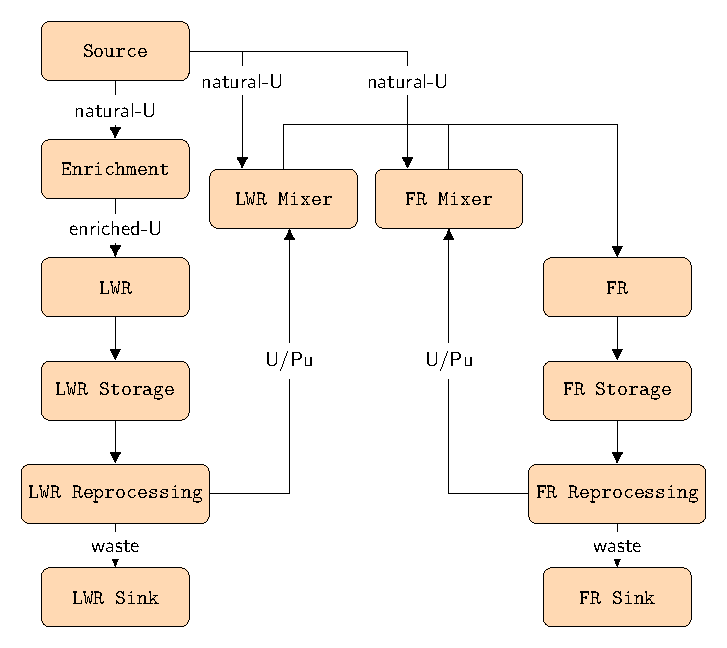
\includegraphics[width=\textwidth]{23-figures/23flow.pdf} 
	\hfill
	\caption{Diagram with facilities and mass flow of the scenario EG01-EG23.}
	\label{fig:23flow}
\end{figure}

\subsection{Flat Power Demand: Power}

This section presents plots of power for all the prediction methods. 
The power demand is 60000 MW throughout the whole simulation. 
Table \ref{tab:23-inputs} shows the input parameters. 
Figures \ref{fig:23-NO}, \ref{fig:23-DO}, and \ref{fig:23-SO} display the power 
demand and corresponding supply from the Non-optimizing (NO), Deterministic-optimizing (DO), 
and Stochastic-optimizing methods (SO), respectively. 
The plots only show the power demand and supply during the transition period as 
undersupply mostly occurs during the transition period. 
Undersupply of power occurs during two main time periods:  
initial demand for the commodity and during the transition period. 
Undersupply time steps occurring at the beginning of the simulation 
is expected since without time series data at the beginning of the simulation, 
\deploy takes a few time steps to collect time series data about power demand 
to begin predicting and starting the deployment of reactor and supporting fuel 
cycle facilities. 
Table \ref{tab:23-power} records the number of steps with undersupply, 
the cumulative undersupply, and the cumulative oversupply for 
each prediction method simulation.  
Cumulative undersupply and cumulative oversupply represent the 
summation of the difference between the power supplied and the power demanded 
for all the time steps in the simulation. 
This magnitude could be best understood as energy. 
The cumulative undersupply represents the energy not provided 
during the time steps in which the supply did not meet the demand. 
Likewise, the oversupply is the excess of energy produced.
In table \ref{tab:23-power} we see that the smallest cumulative under 
supply and smallest amount of undersupply time steps are for poly and fft
prediction methods.


\begin{table}[H]
	\centering
	\caption{EG01-EG23 input file values.}
	\label{tab:23-inputs}
	\begin{tabularx}{\textwidth}{lR}
		\hline
		Parameter			& Value \\ 	\hline
		Demand equation		& 6e4  \\
		Deployment Driving Method 	& Installed Capacity \\
		Buffer    			& 0 \\
		Forward Steps		& 1 \\
		Backward Steps		& 2 \\		\hline
	\end{tabularx}
\end{table}

\begin{figure}[H]
	\centering
	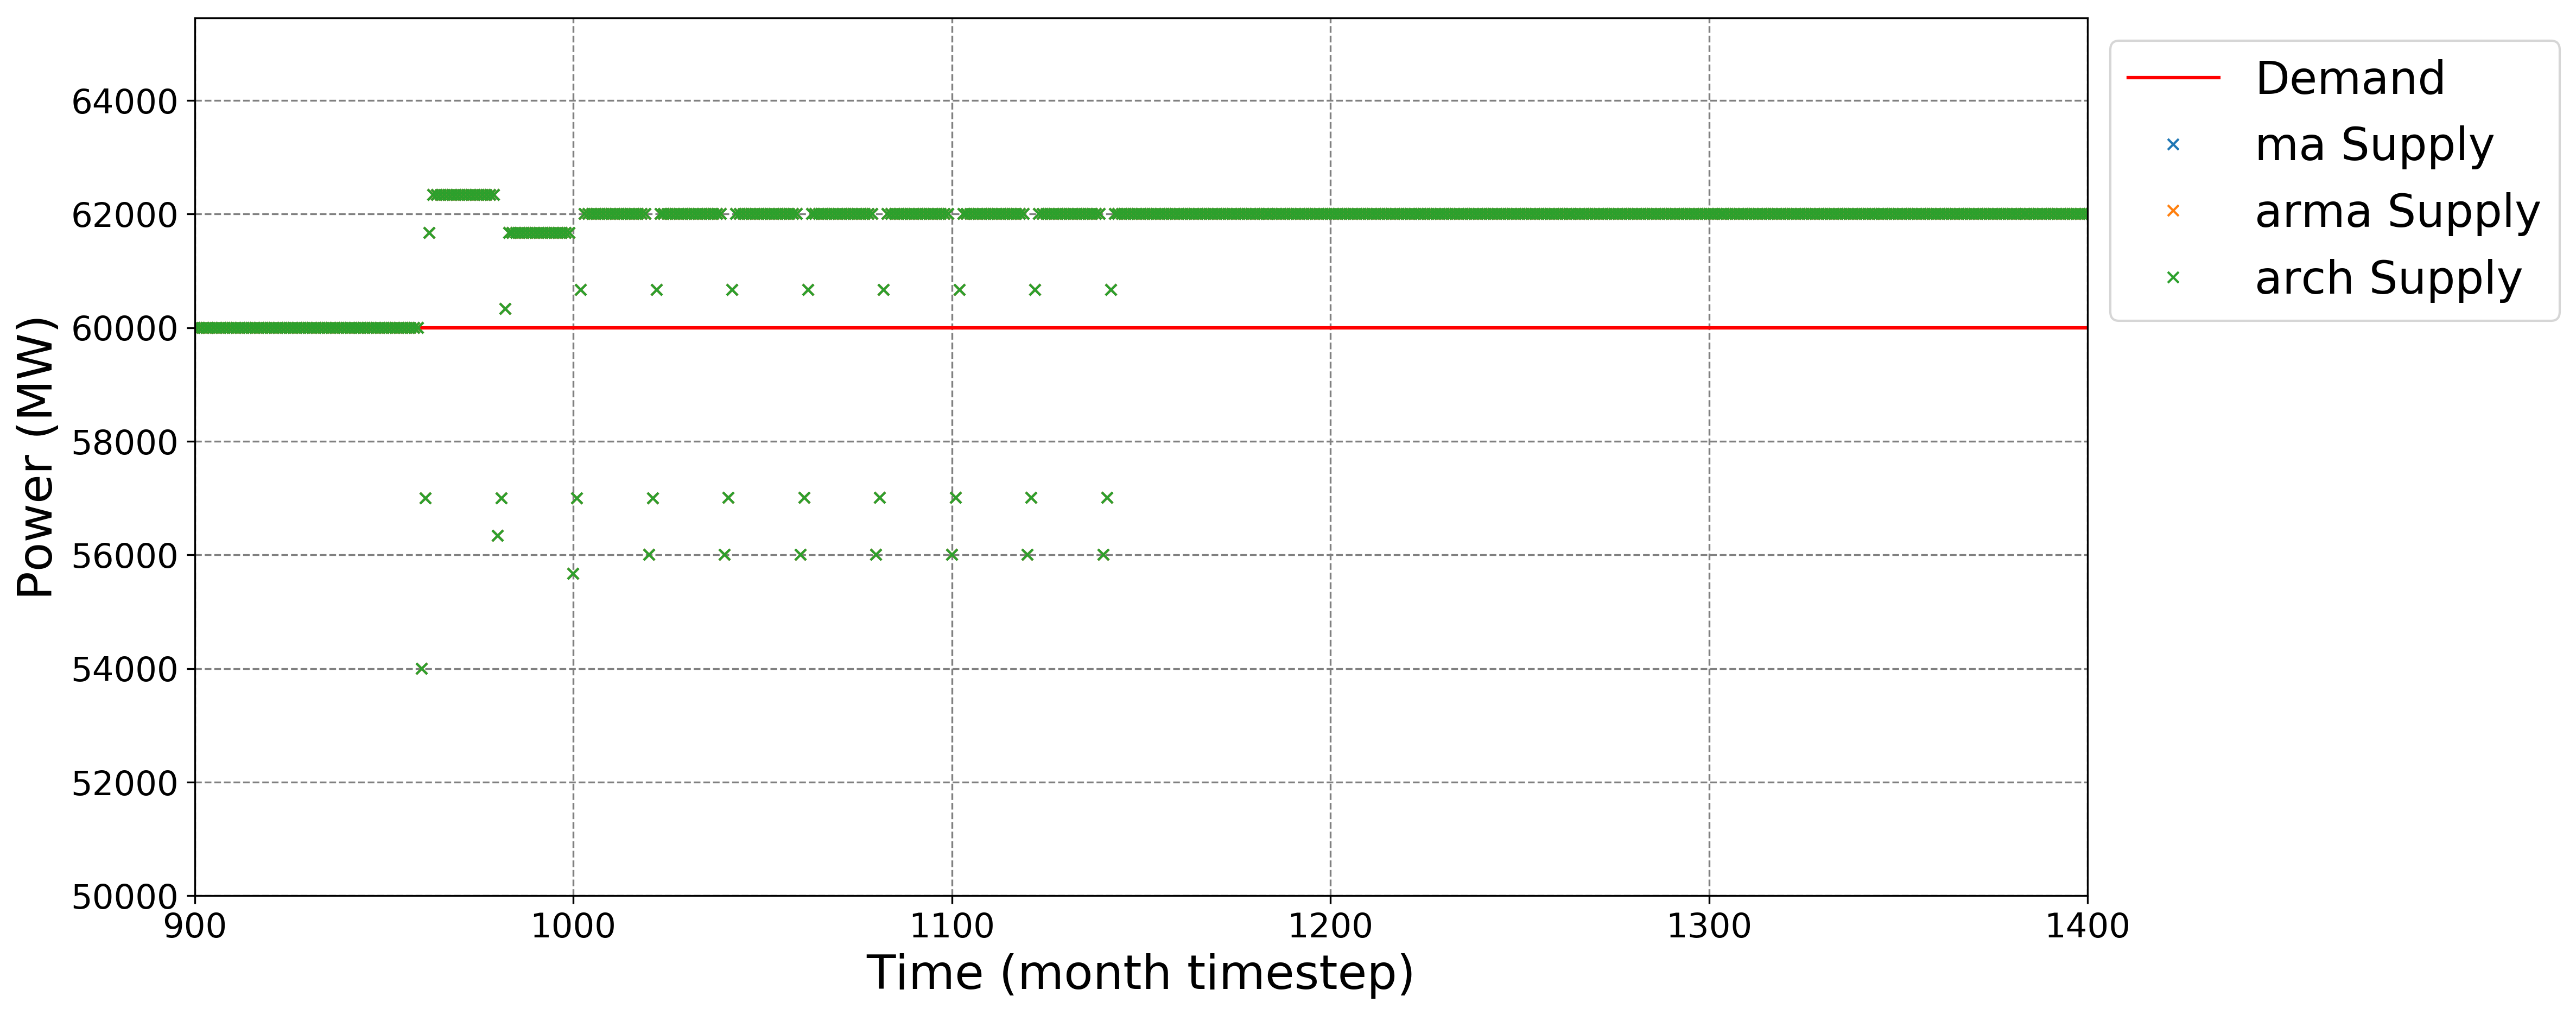
\includegraphics[width=\textwidth]{23-figures/23-power0-buffer01.png} 
	\hfill
	\caption{Constant power demand of 60GW and power supply obtained with the NO algorithms.}
	\label{fig:23-NO}
\end{figure}

\begin{figure}[H]
	\centering
	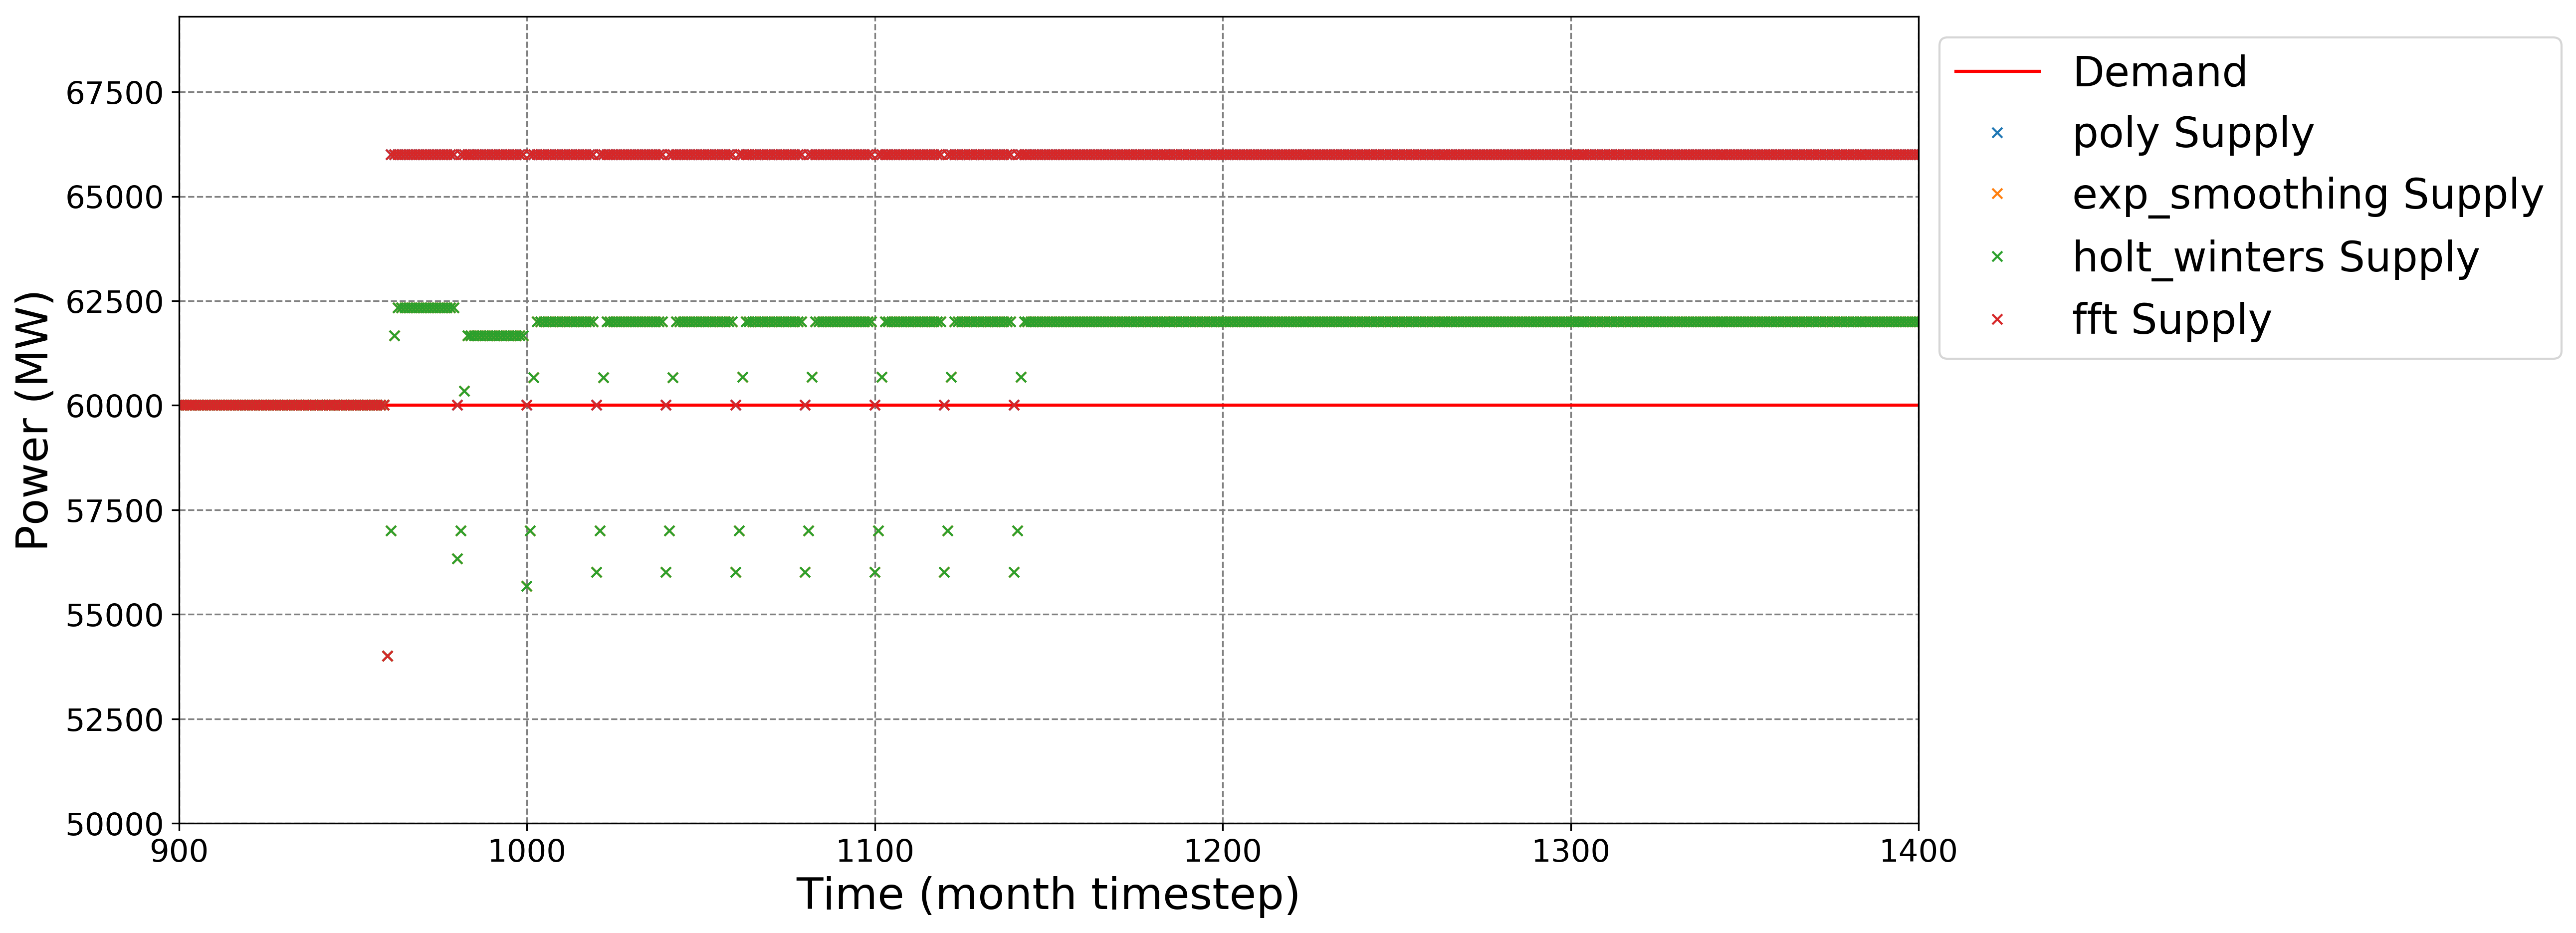
\includegraphics[width=\textwidth]{23-figures/23-power0-buffer02.png} 
	\hfill
	\caption{Constant power demand of 60GW and power supply obtained with the DO algorithms.}
	\label{fig:23-DO}
\end{figure}

\begin{figure}[H]
	\centering
	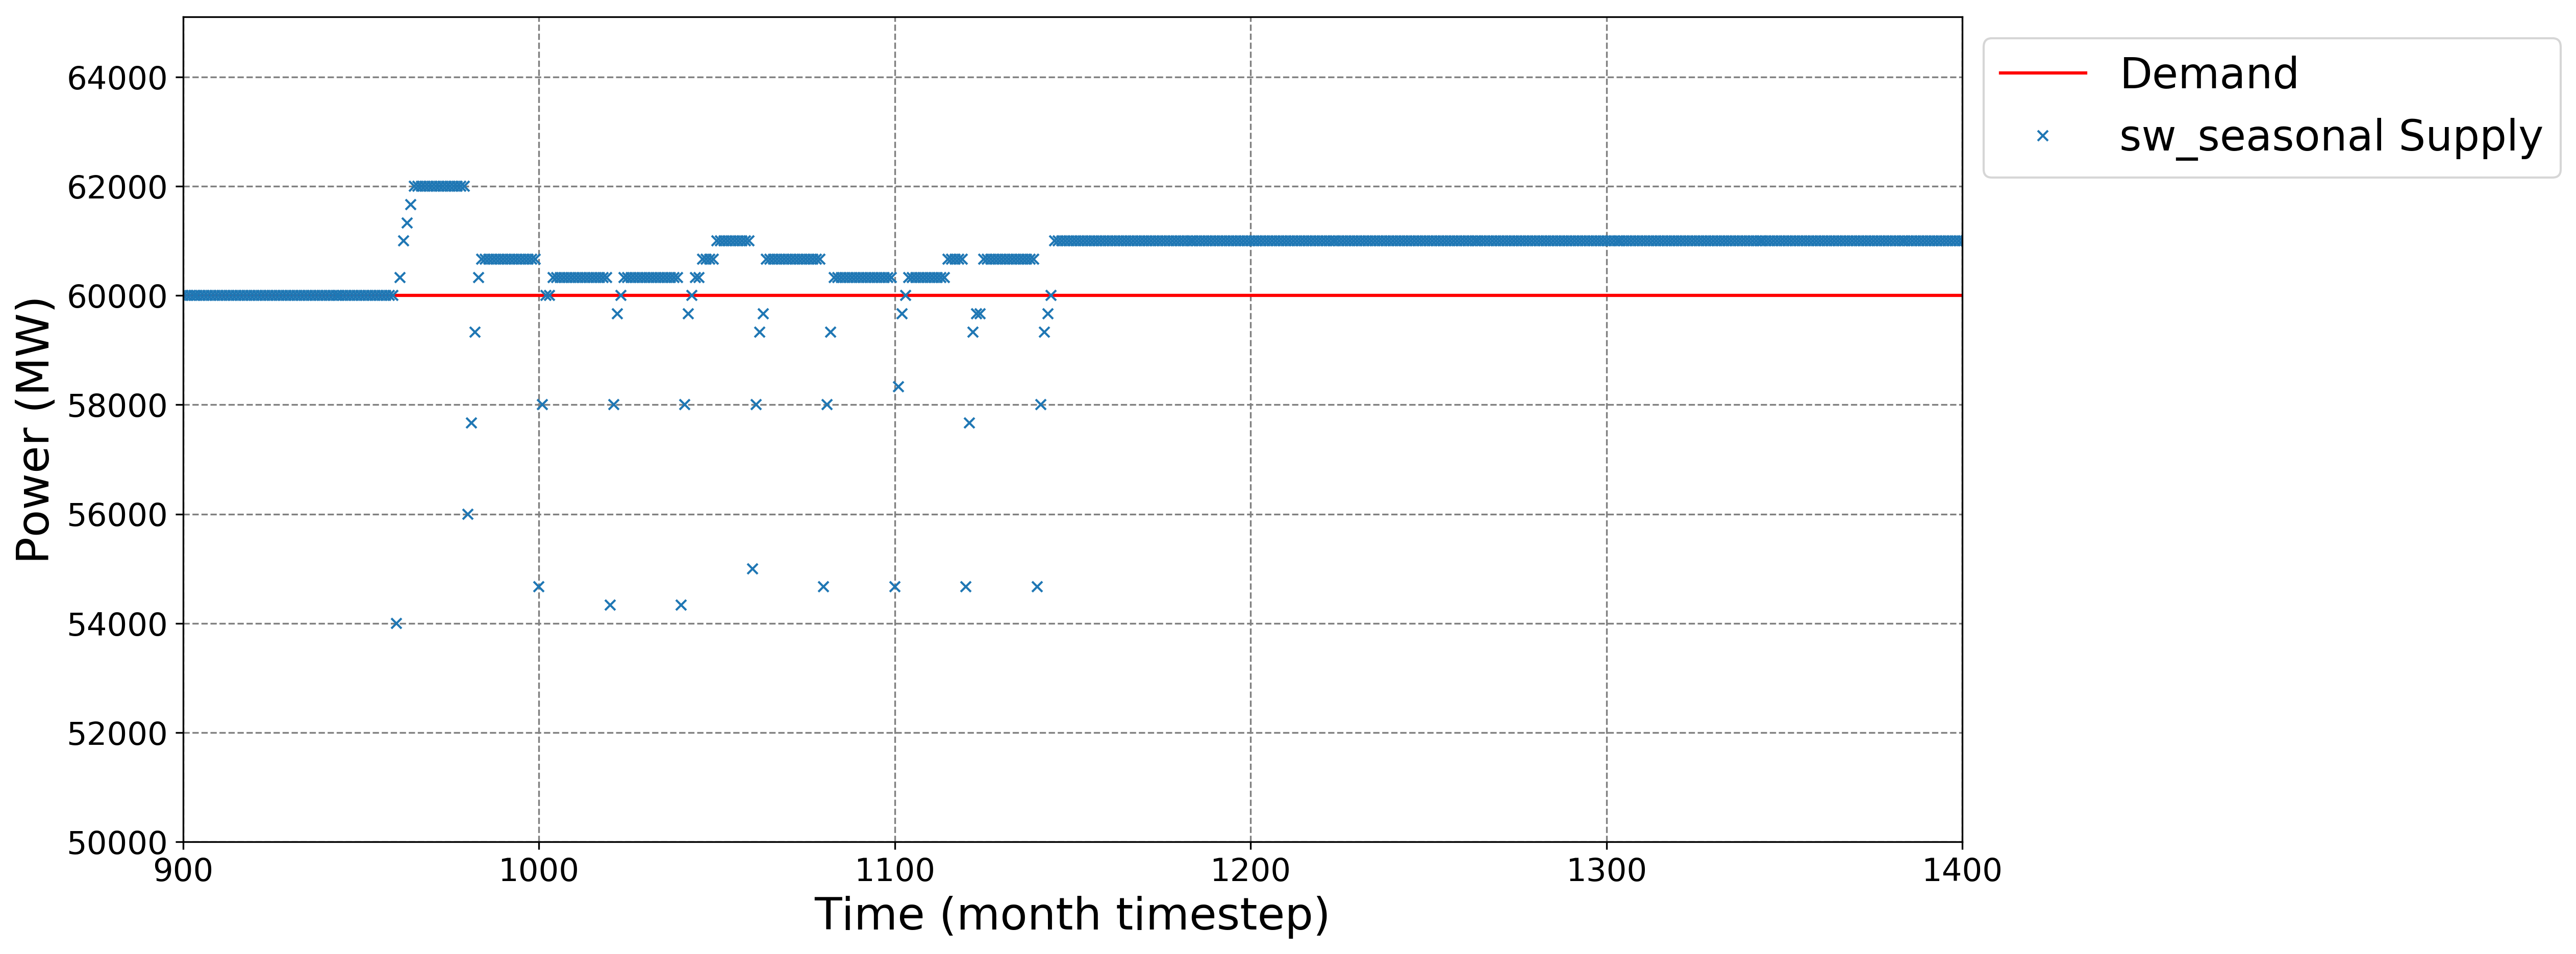
\includegraphics[width=\textwidth]{23-figures/23-power0-buffer03.png} 
	\hfill
	\caption{Constant power demand of 60GW and power supply obtained with the SO algorithms.}
	\label{fig:23-SO}
\end{figure}

\begin{table}[H]
	\centering
	\caption{Undersupply and oversupply of Power for the different prediction algorithms used to calculate EG01-EG23.}
	\label{tab:23-power}
	\begin{tabularx}{\textwidth}{lRRR}
		\hline
		Algorithm & Undersupplied & Cumulative  & Cumulative \\
		& Timesteps     & Undersupply [GW.mo]  & Oversupply [GW.mo] \\ \hline
		MA        & 26 	& 306.0 &  907.8   \\ 
		ARMA      & 26 	& 306.0 &  907.8   \\ 
		ARCH      & 26 	& 306.0 &  907.8   \\ 
		POLY      &  6 	& 235.0 &  2820.5  \\ 
		EXP\_SMOOTHING 	& 27 & 366.0 & 907.8 \\ 
		HOLT-WINTERS  	& 27 & 366.0 & 907.8 \\ 
		FFT       & 8	& 307.0	& 2820.5 \\ 
		SW\_SEASONAL    & 36 & 308.0 & 398.1	\\ \hline
	\end{tabularx}
\end{table}

\subsection{Sensitivity Analysis: Power Buffer}

This section presents a sensitivity analysis for different values of the power buffer. 
Figure \ref{fig:23-buff} shows a comparison of the cumulative undersupply for 
different buffer sizes for different prediction methods. 
The cumulative undersupply, remains constant for some of the methods and 
decreases with the increase of the buffer for others. 
Figure \ref{fig:23-buf-poly} displays the power demand and supply for
different values of the buffer using poly. 
For this case, the undersupply remains constant. 
Figure \ref{fig:23-buf-poly} helps to understand the observed behavior. 
During at the transition we can see that even for the buffer with size 
0 MW there is no undersupply. 
Thus, increasing the buffer will not decrease an undersupply that is 
already zero.

\begin{figure}[H]
	\centering
	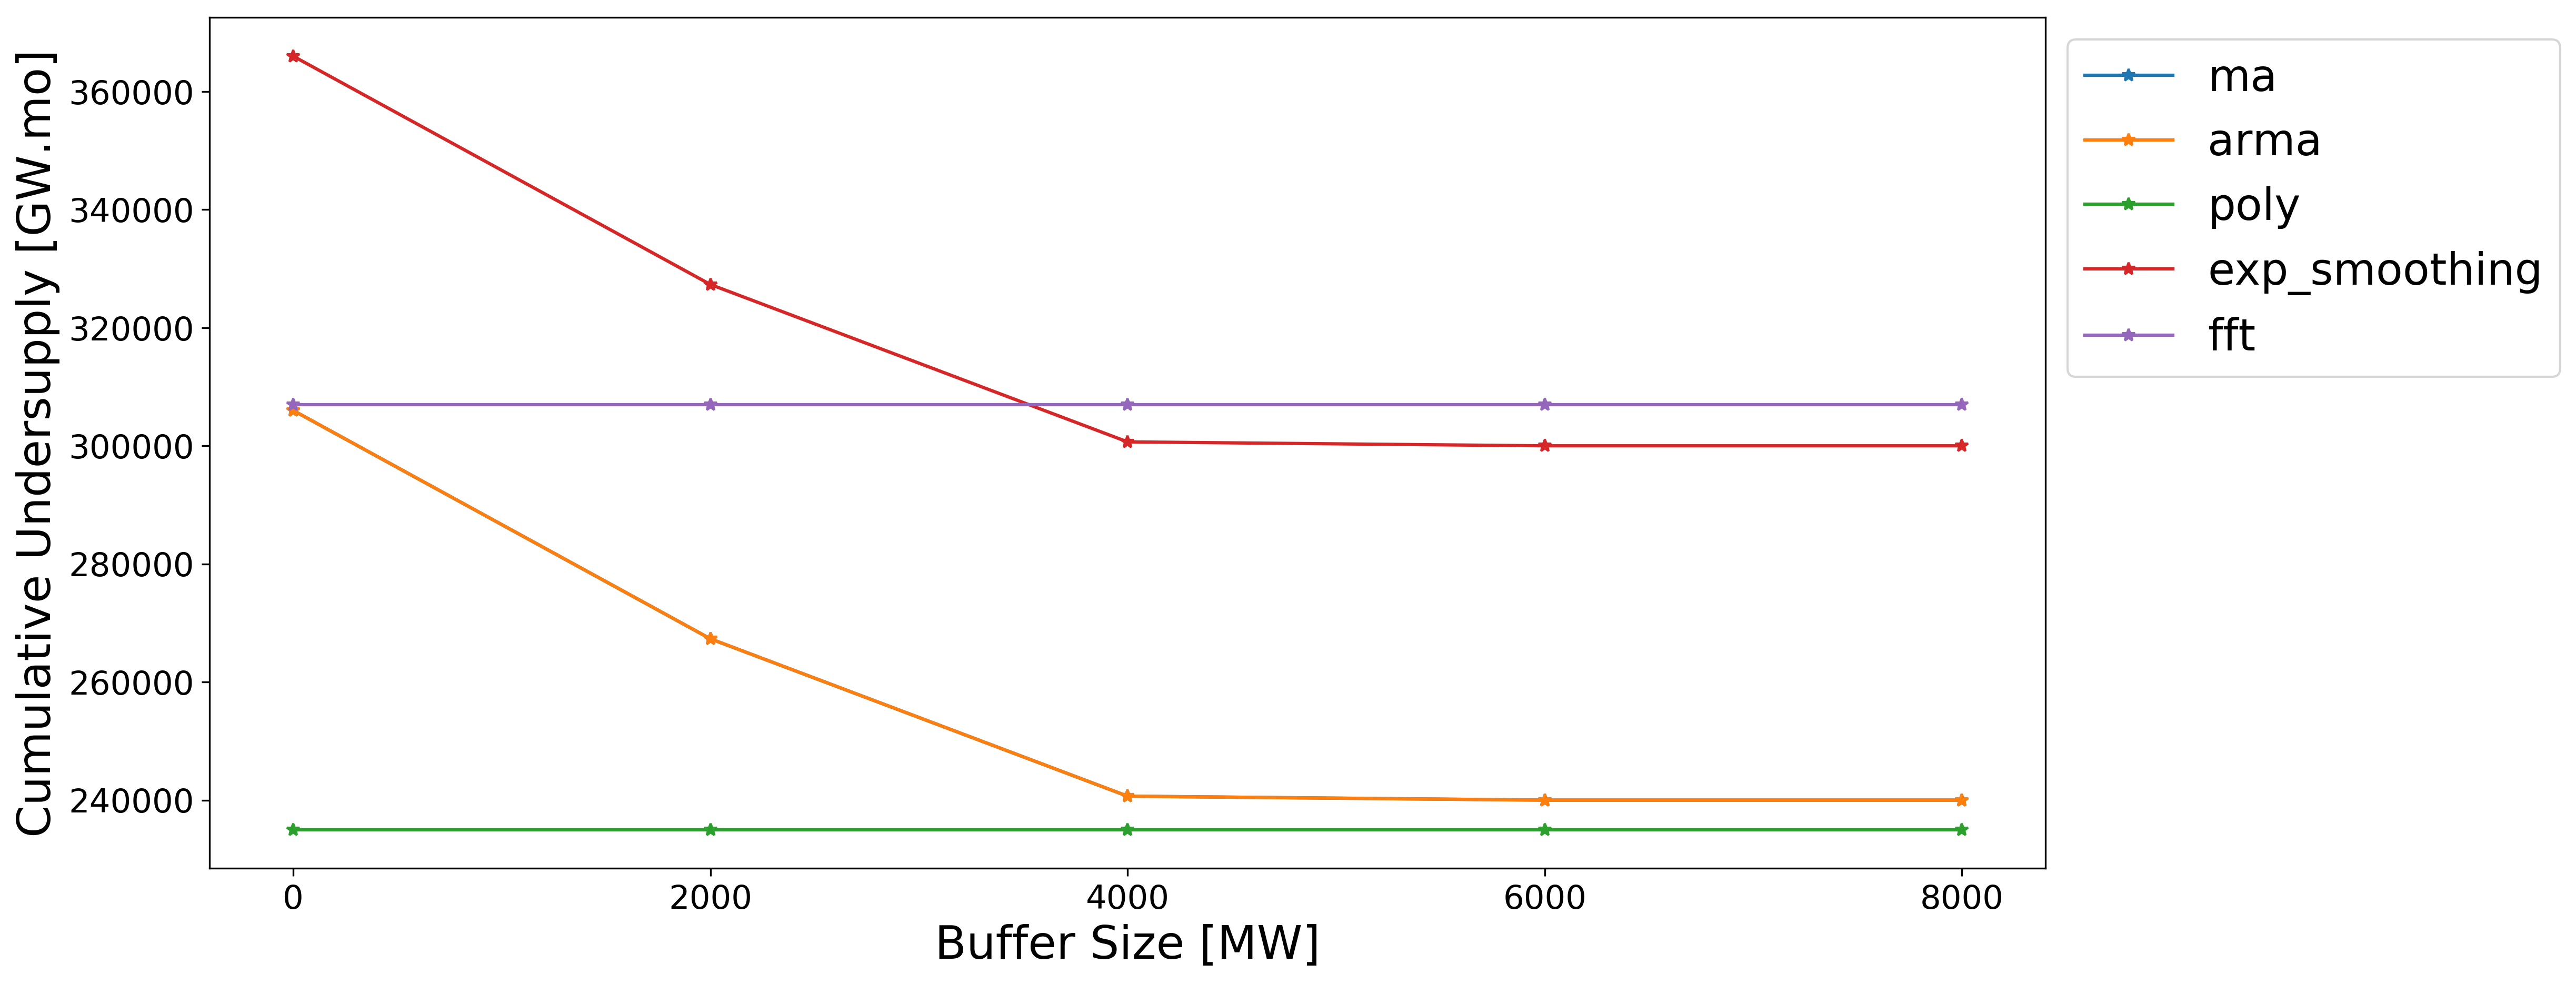
\includegraphics[width=\textwidth]{23-figures/23-sens-buffer.png} 
	\hfill
	\caption{Sensitivity analysis for different buffer sizes for different prediction algorithms.}
	\label{fig:23-buff}
\end{figure}

\begin{figure}[H]
	\centering
	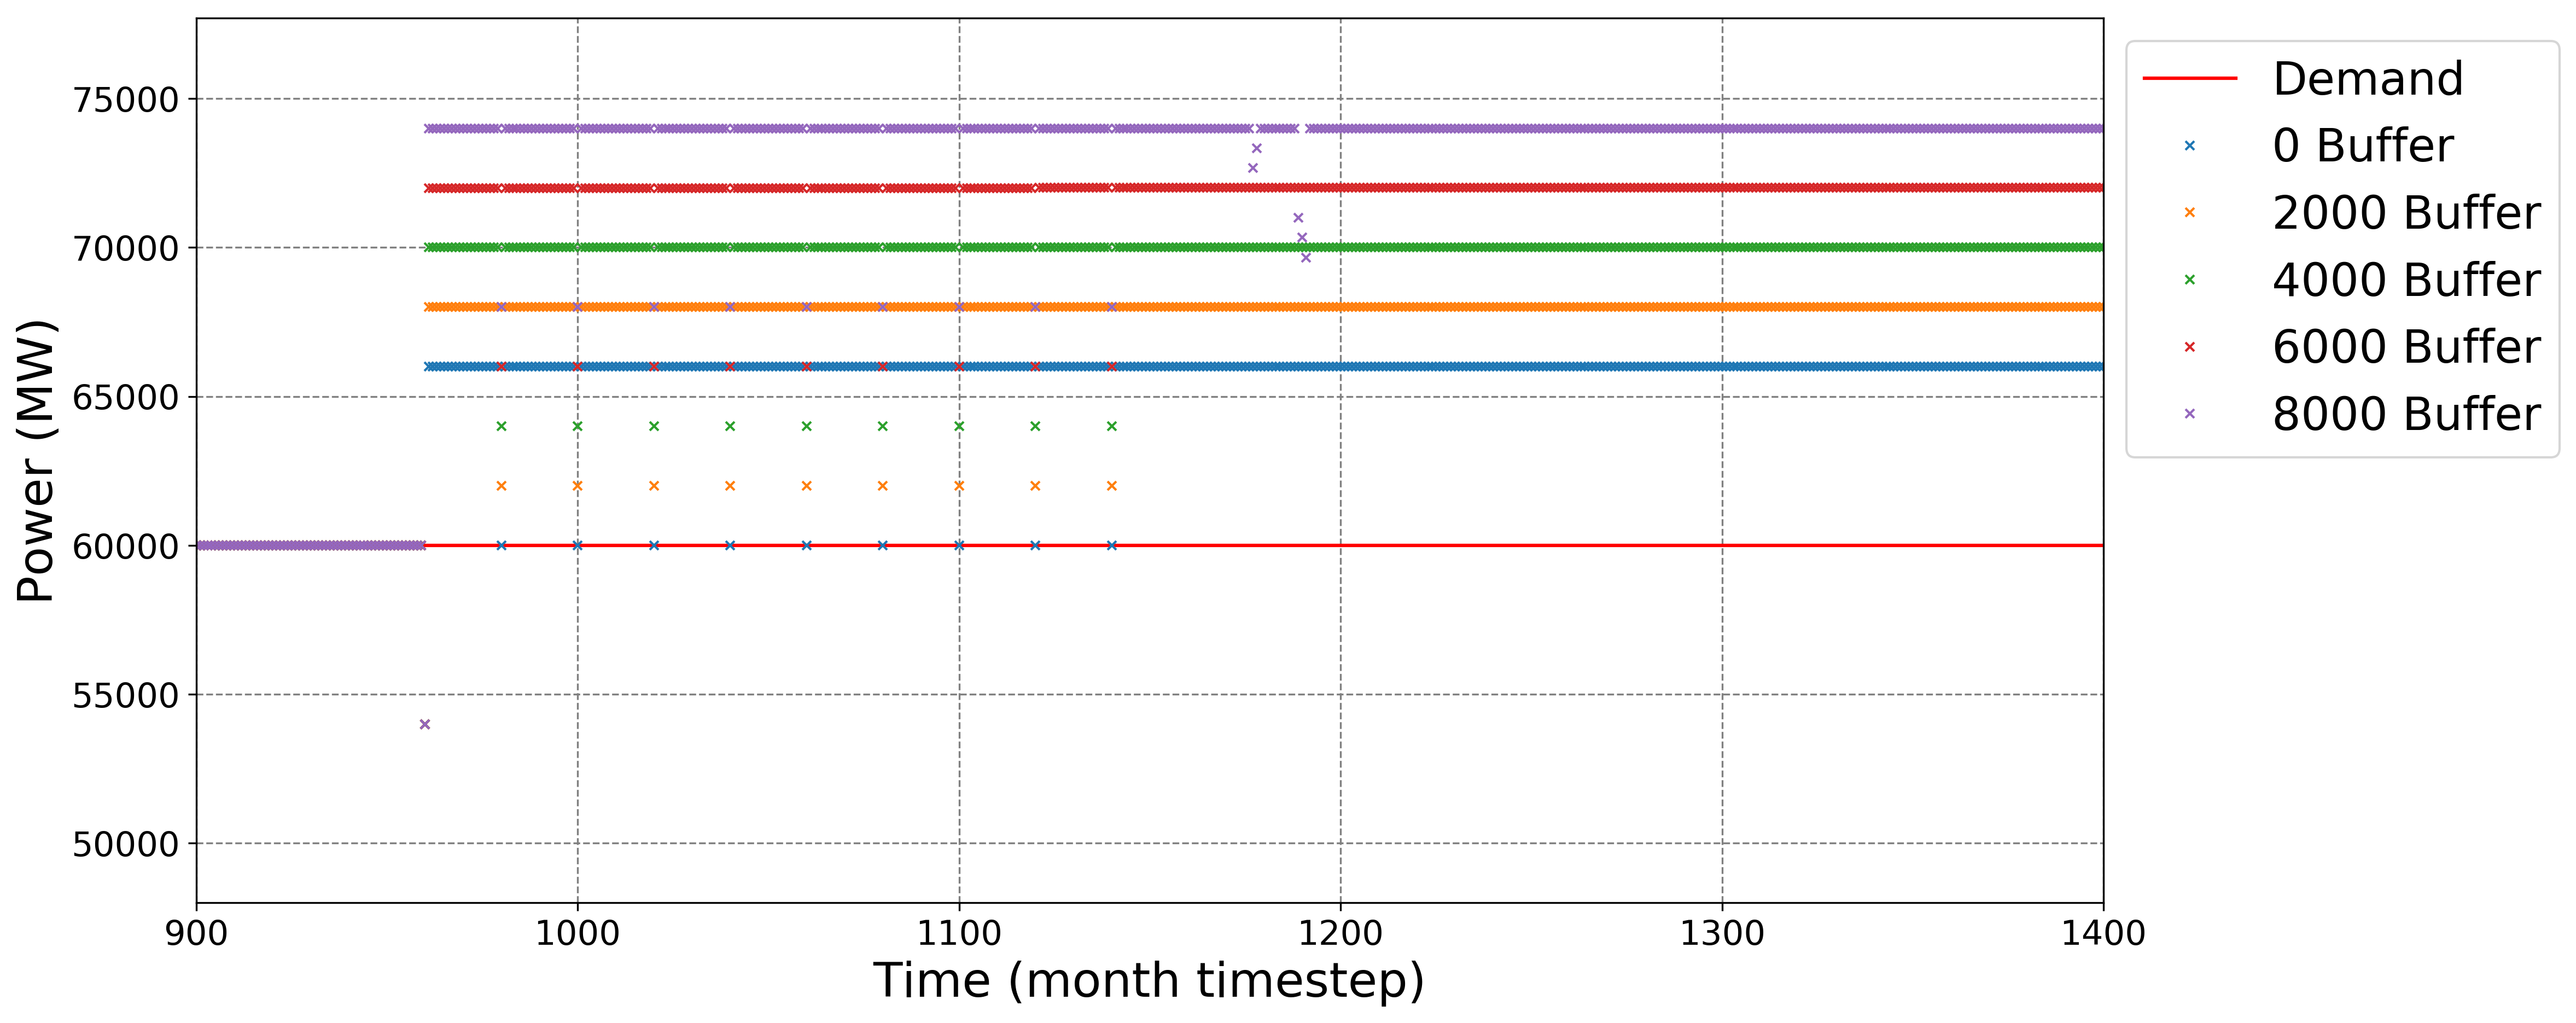
\includegraphics[width=\textwidth]{23-figures/23-power-buffer-poly.png} 
	\hfill
	\caption{Power supply for different buffer sizes using poly.}
	\label{fig:23-buf-poly}
\end{figure}

\subsection{Sensitivity Analysis: Forward Steps}

This section presents a sensitivity analysis for different number of forward steps.
Figure \ref{fig:23-steps} shows a plot of the cumulative undersupply 
varying number of forward steps using the poly prediction method.
Slightly increasing the number of forward steps decreases the undersupply. 
Increasing the number of forward steps too much has a negative impact on the results.
Figure \ref{fig:23-ste-poly} displays the plots for power supply for different 
number of forward steps. For 4 and 5 forward steps, the undersupply increases.
Increasing the number of forward steps enlarges the production of power, 
more reactors are deployed and consequently, the new reactors require more fuel. 
As they require more fuel, the available fuel will not be enough,
and the scenario will fail. 
Figure \ref{fig:23-ste-fft-mixerout} helps to understand this behavior. 
This figure shows that the demand of fuel for the FRs is larger than the 
supply of the same commodity.
The forward steps capability should be used only with small number of forward steps 
to avoid this undersupply from occurring. 

\begin{figure}[H]
	\centering
	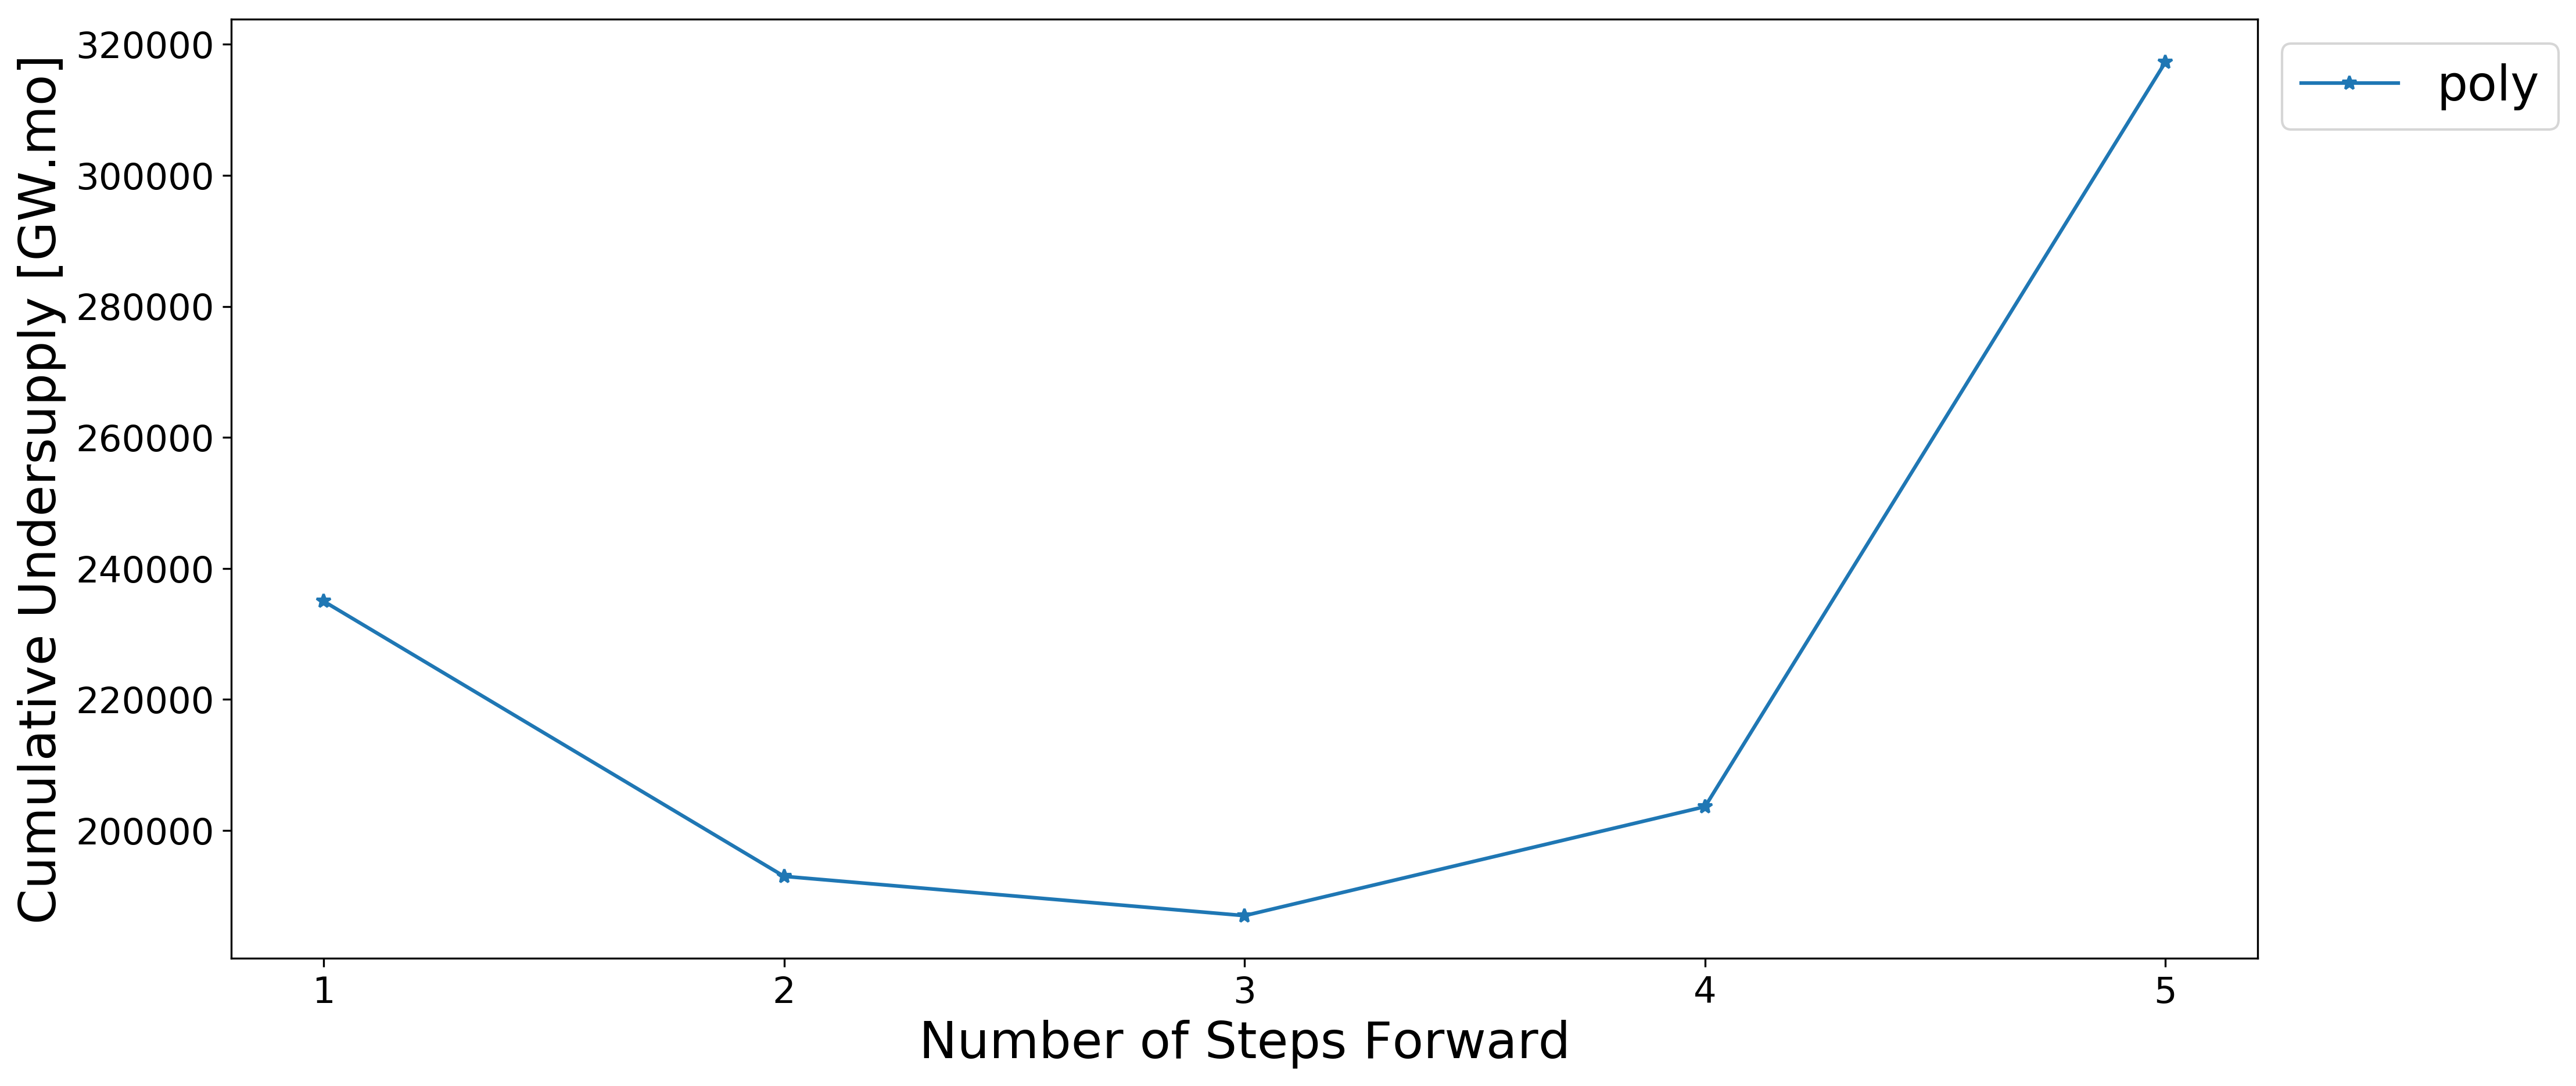
\includegraphics[width=\textwidth]{23-figures/23-sens-steps.png} 
	\hfill
	\caption{Cumulative undersupply varying the number of forward steps using the poly prediction method.}
	\label{fig:23-steps}
\end{figure}

\begin{figure}[H]
	\centering
	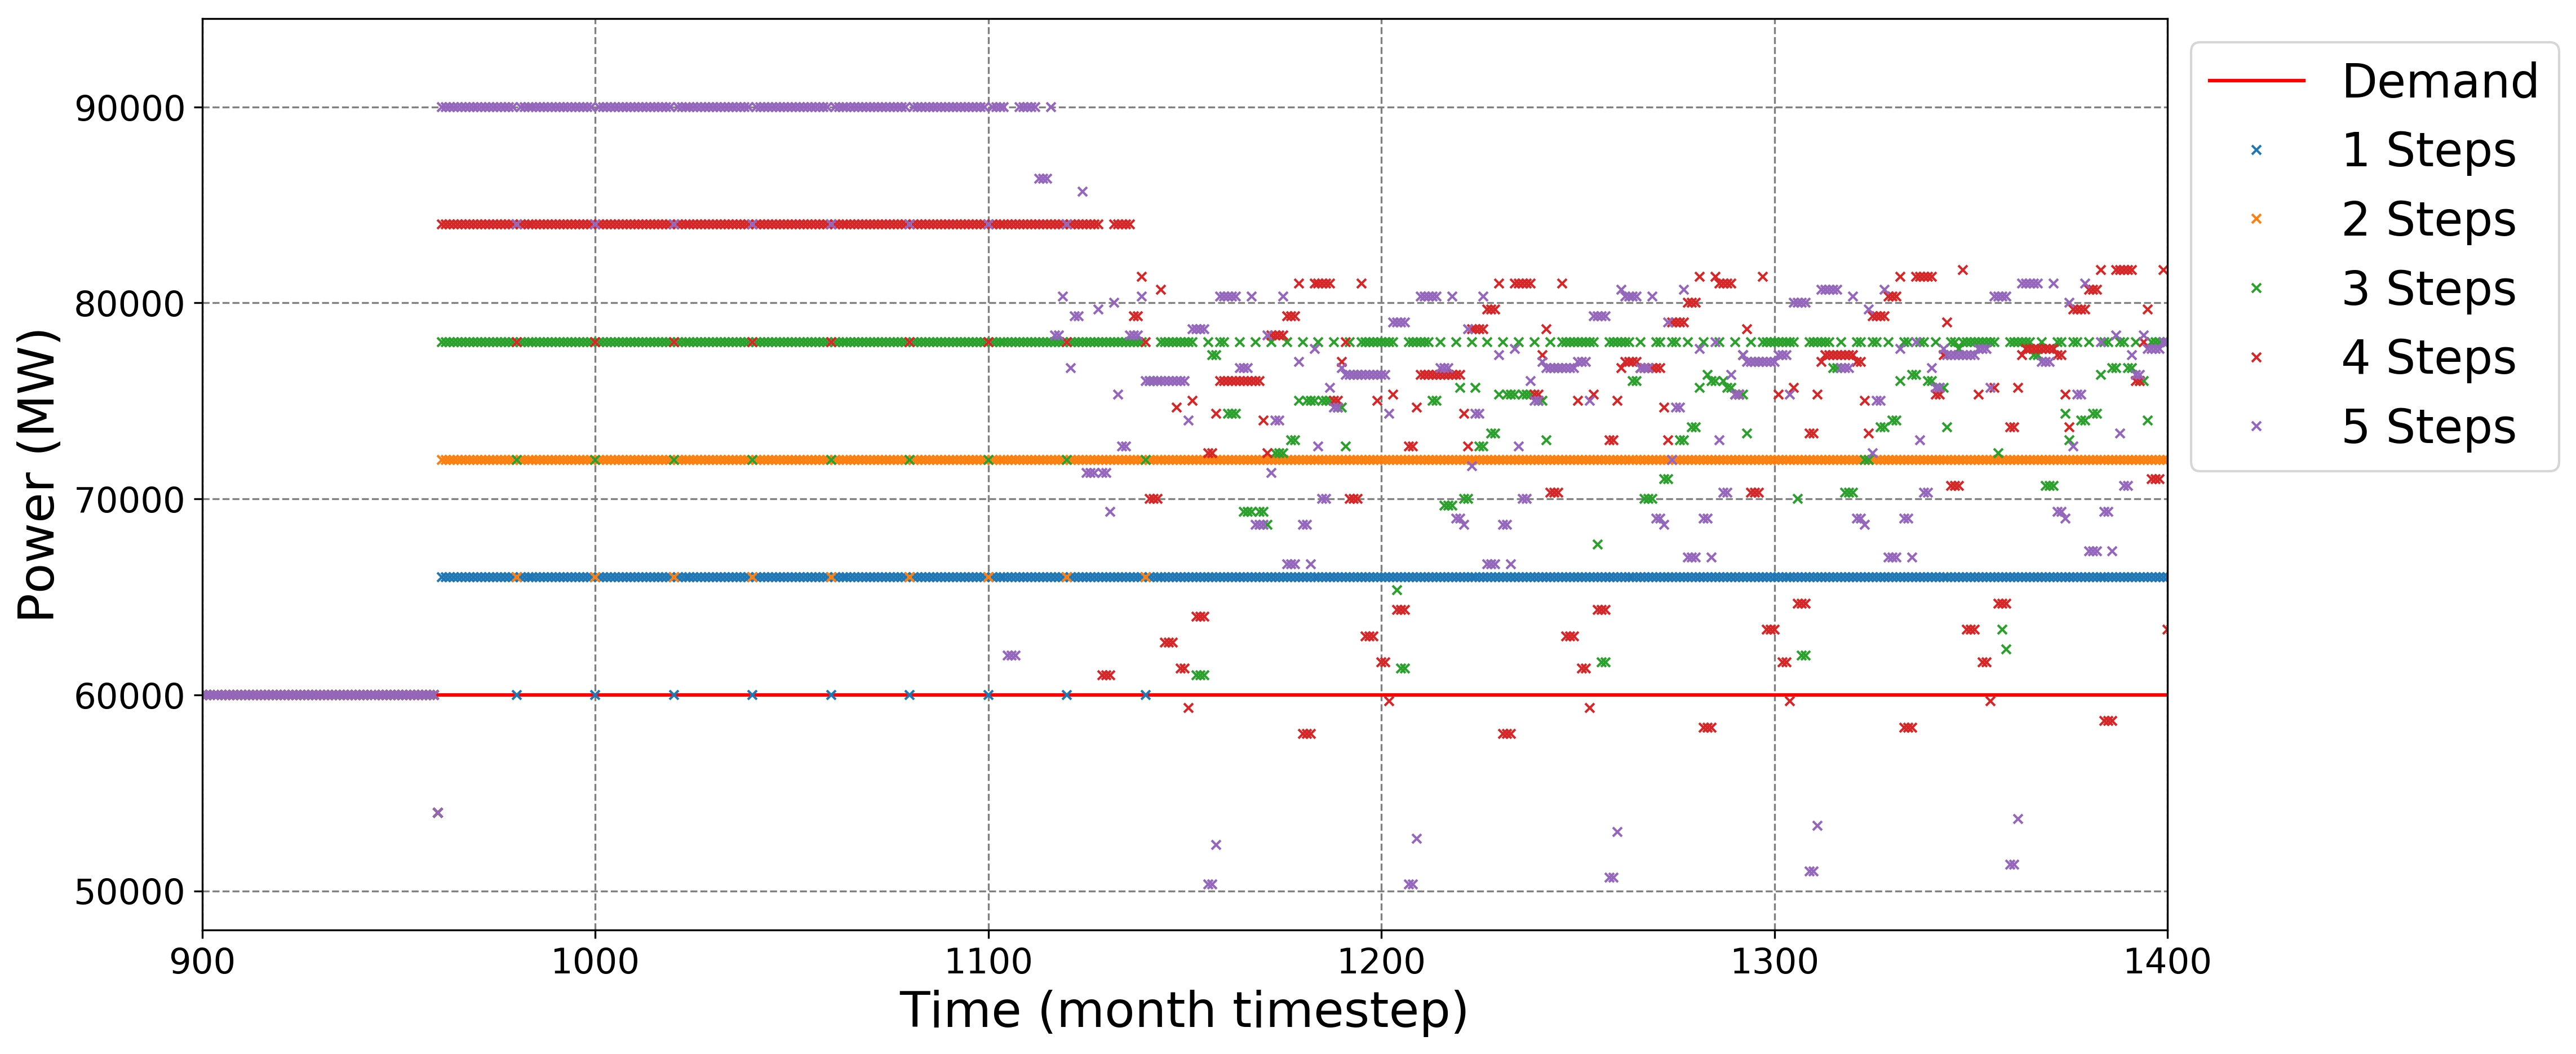
\includegraphics[width=\textwidth]{23-figures/23-power-buffer0-poly-steps.png} 
	\hfill
	\caption{Power supply varying the number of forward steps using the poly prediction method.}
	\label{fig:23-ste-poly}
\end{figure}

\begin{figure}[H]
	\centering
	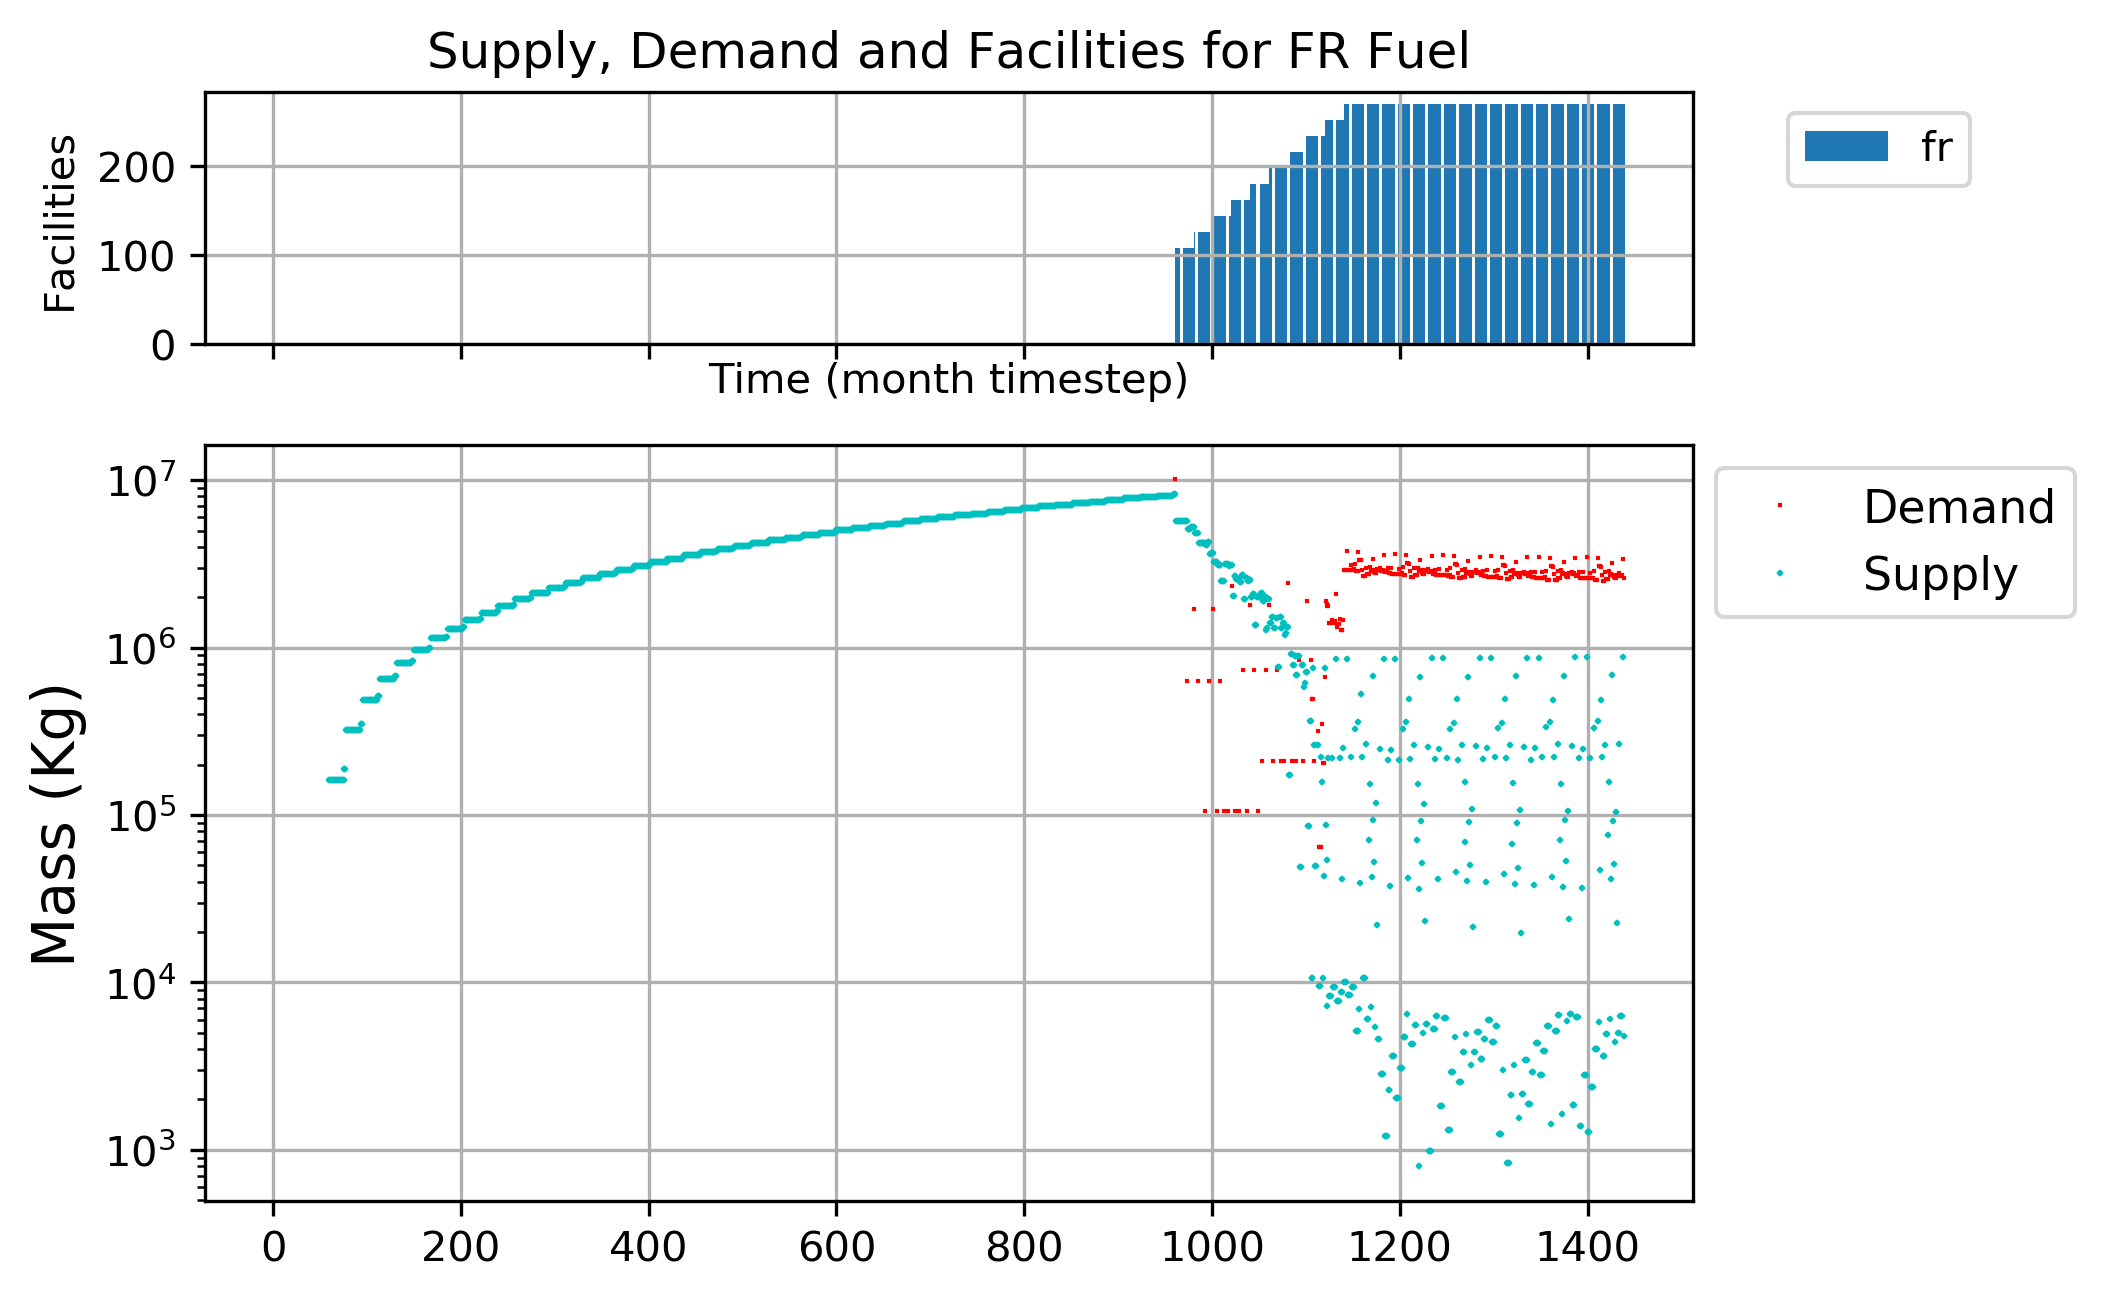
\includegraphics[width=\textwidth]{23-figures/0-S5-poly-mixerout.png} 
	\hfill
	\caption{Power supply for 5 forward steps using the poly prediction method.}
	\label{fig:23-ste-fft-mixerout}
\end{figure}

\subsection{Flat Power Demand: Meaningful Commodities}
Using the best prediction method, poly, this section presents plots 
for the supply and demand of the most meaningful commodities in the transition scenario.
Table \ref{tab:23-commodities} summarizes which commodity each figure in this section 
corresponds to.
Table \ref{tab:23-commod} presents the number of steps of undersupply, 
cumulative undersupply, and cumulative oversupply for each commodity.

\begin{table}[H]
	\centering
	\caption{Table of figures of commodities in the simulation of EG01-EG23.}
	\label{tab:23-commodities}
	\begin{tabularx}{\textwidth}{lR}
		\hline
		Commodity & Figure \\ \hline
  		Power           & \ref{fig:23-power} \\
		Natural-U       & \ref{fig:23-sourceout} \\
        Enriched-U   	& \ref{fig:23-enrichmentout} \\
        FR fuel       	& \ref{fig:23-mixerout} \\
  		Reprocessed Pu from spent fuel of LWRs & \ref{fig:23-lwrpu} \\
  		Reprocessed Pu from spent fuel of FRs  & \ref{fig:23-frpu} \\ \hline
	\end{tabularx}
\end{table}

\begin{figure}[H]
	\centering
	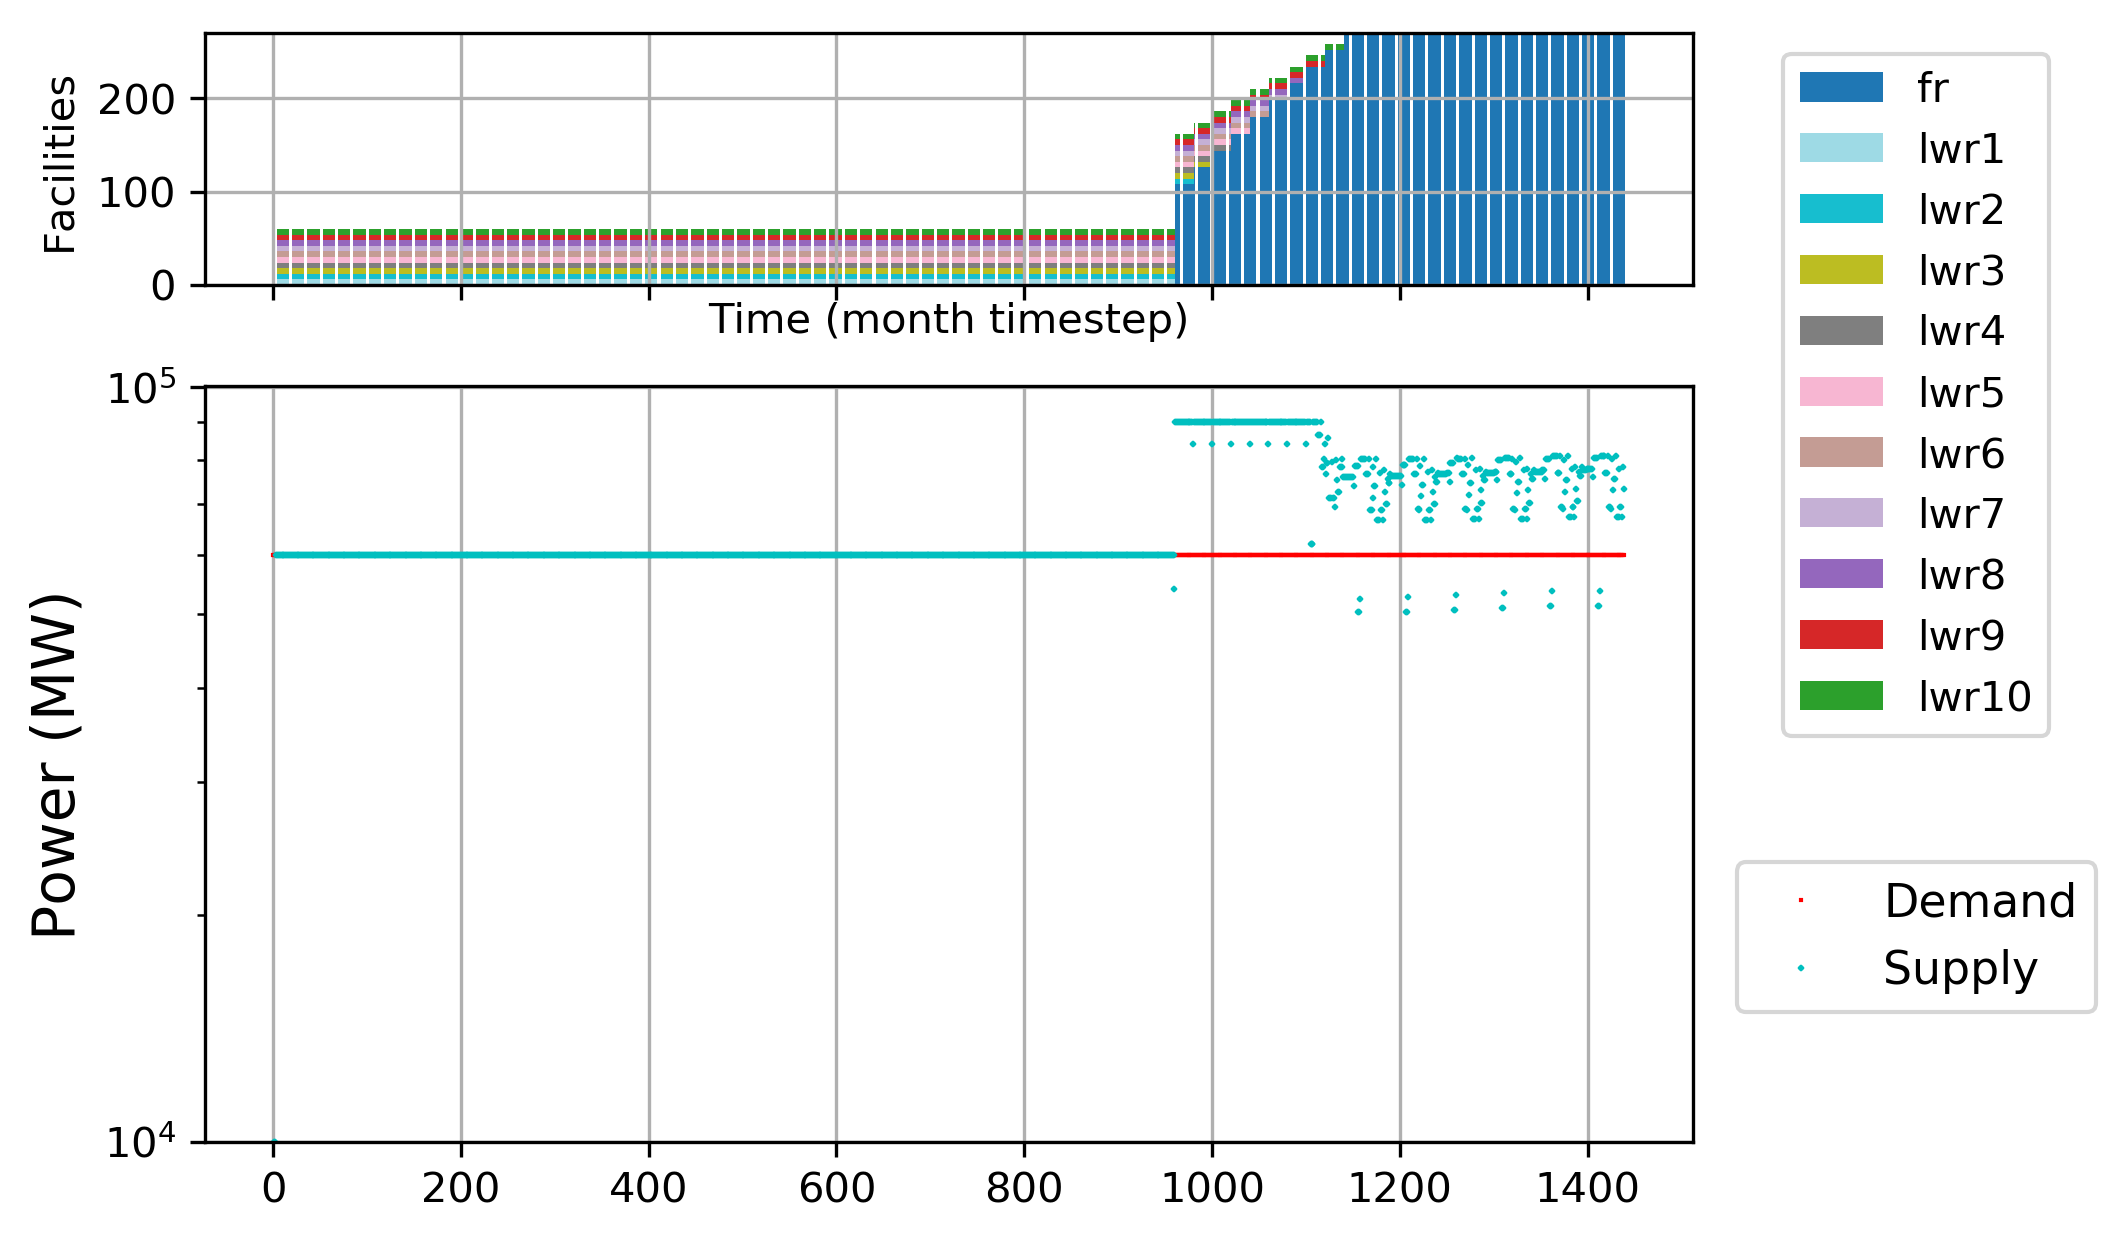
\includegraphics[width=\textwidth]{23-figures/0-poly-power.png} 
	\hfill
	\caption{Demand and supply of Power and number of reactors deployed.}
	\label{fig:23-power}
\end{figure}

\begin{figure}[H]
	\centering
	\begin{subfigure}[]{0.45\textwidth}
		\centering
		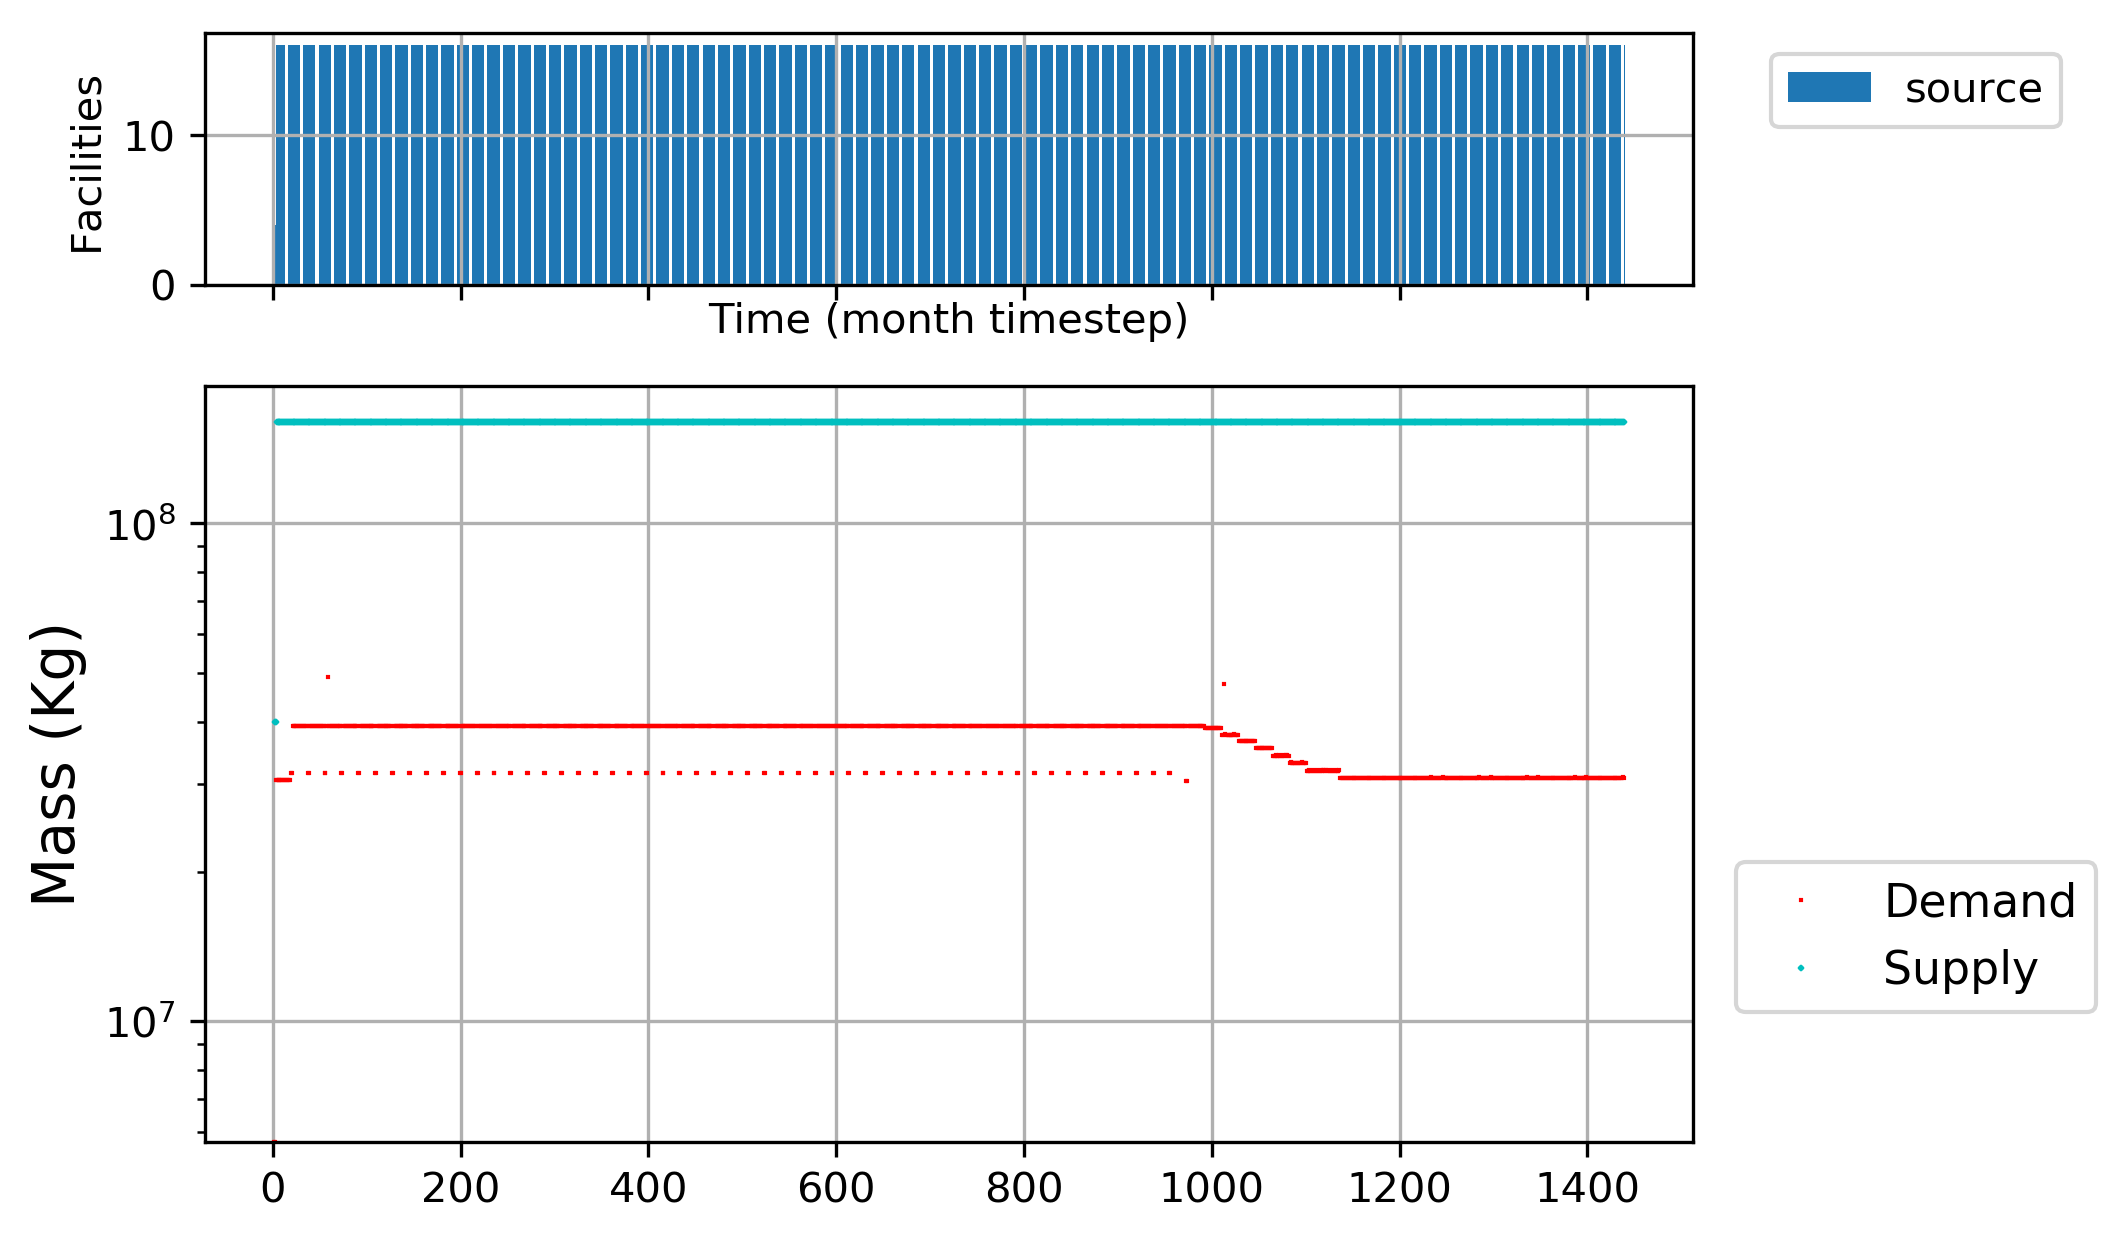
\includegraphics[width=\linewidth]{23-figures/0-poly-sourceout.png} 
		\caption{Natural-U.}
		\label{fig:23-sourceout}
	\end{subfigure}
	\vspace{1cm}
	\begin{subfigure}[]{0.45\textwidth}
		\centering
		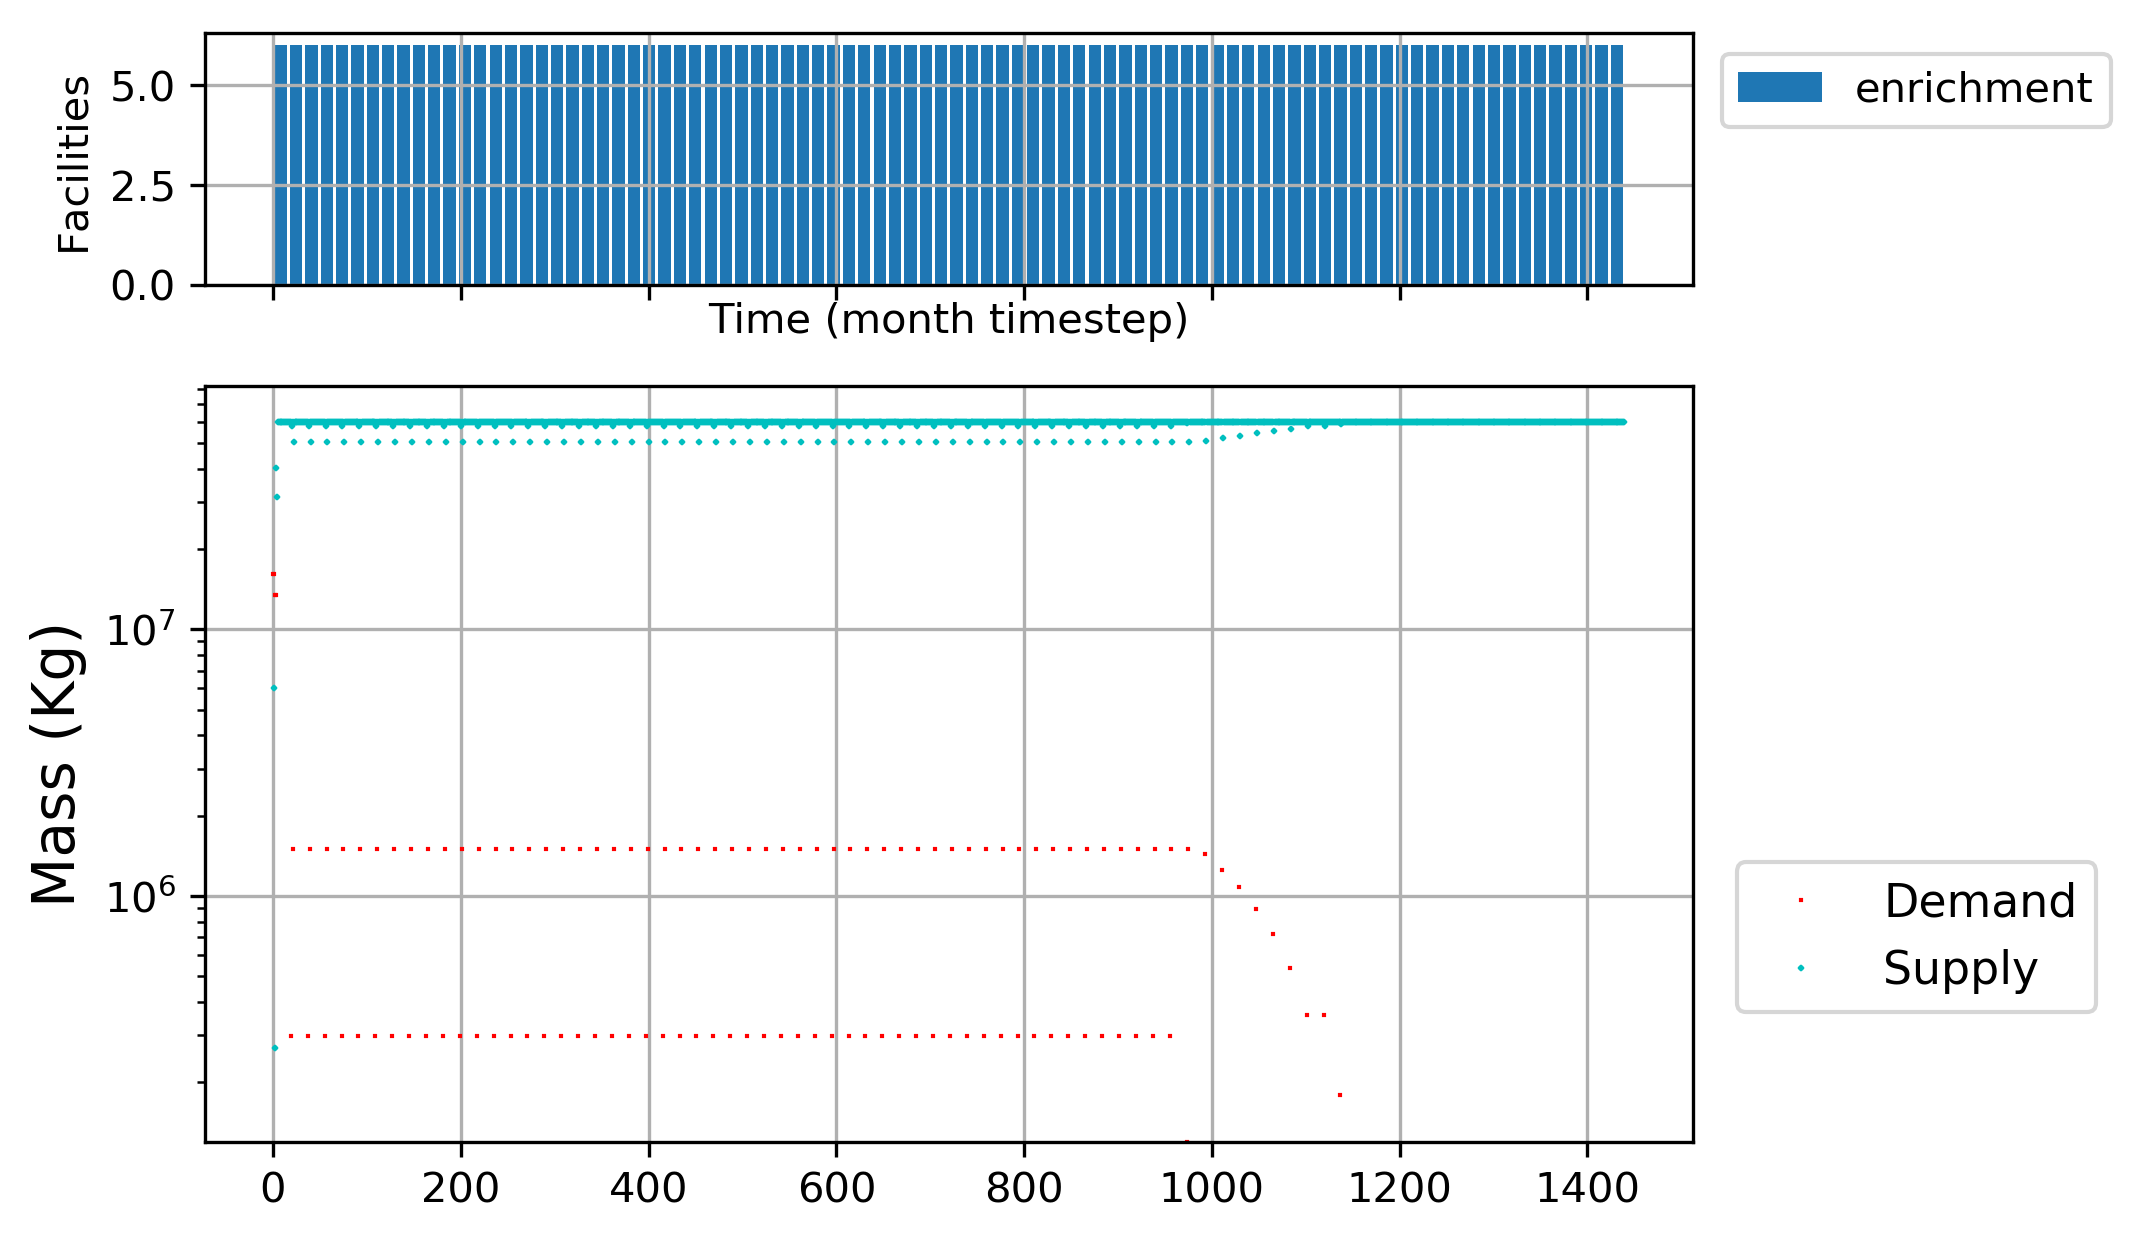
\includegraphics[width=\linewidth]{23-figures/0-poly-enrichmentout.png} 
		\caption{Enriched-U.}
		\label{fig:23-enrichmentout}
	\end{subfigure}
	\hfill
	\caption{Demand and supply of different commodities and number of facilities that produce them.}
	\label{fig:23-front}
\end{figure}

\begin{figure}[H]
	\centering
	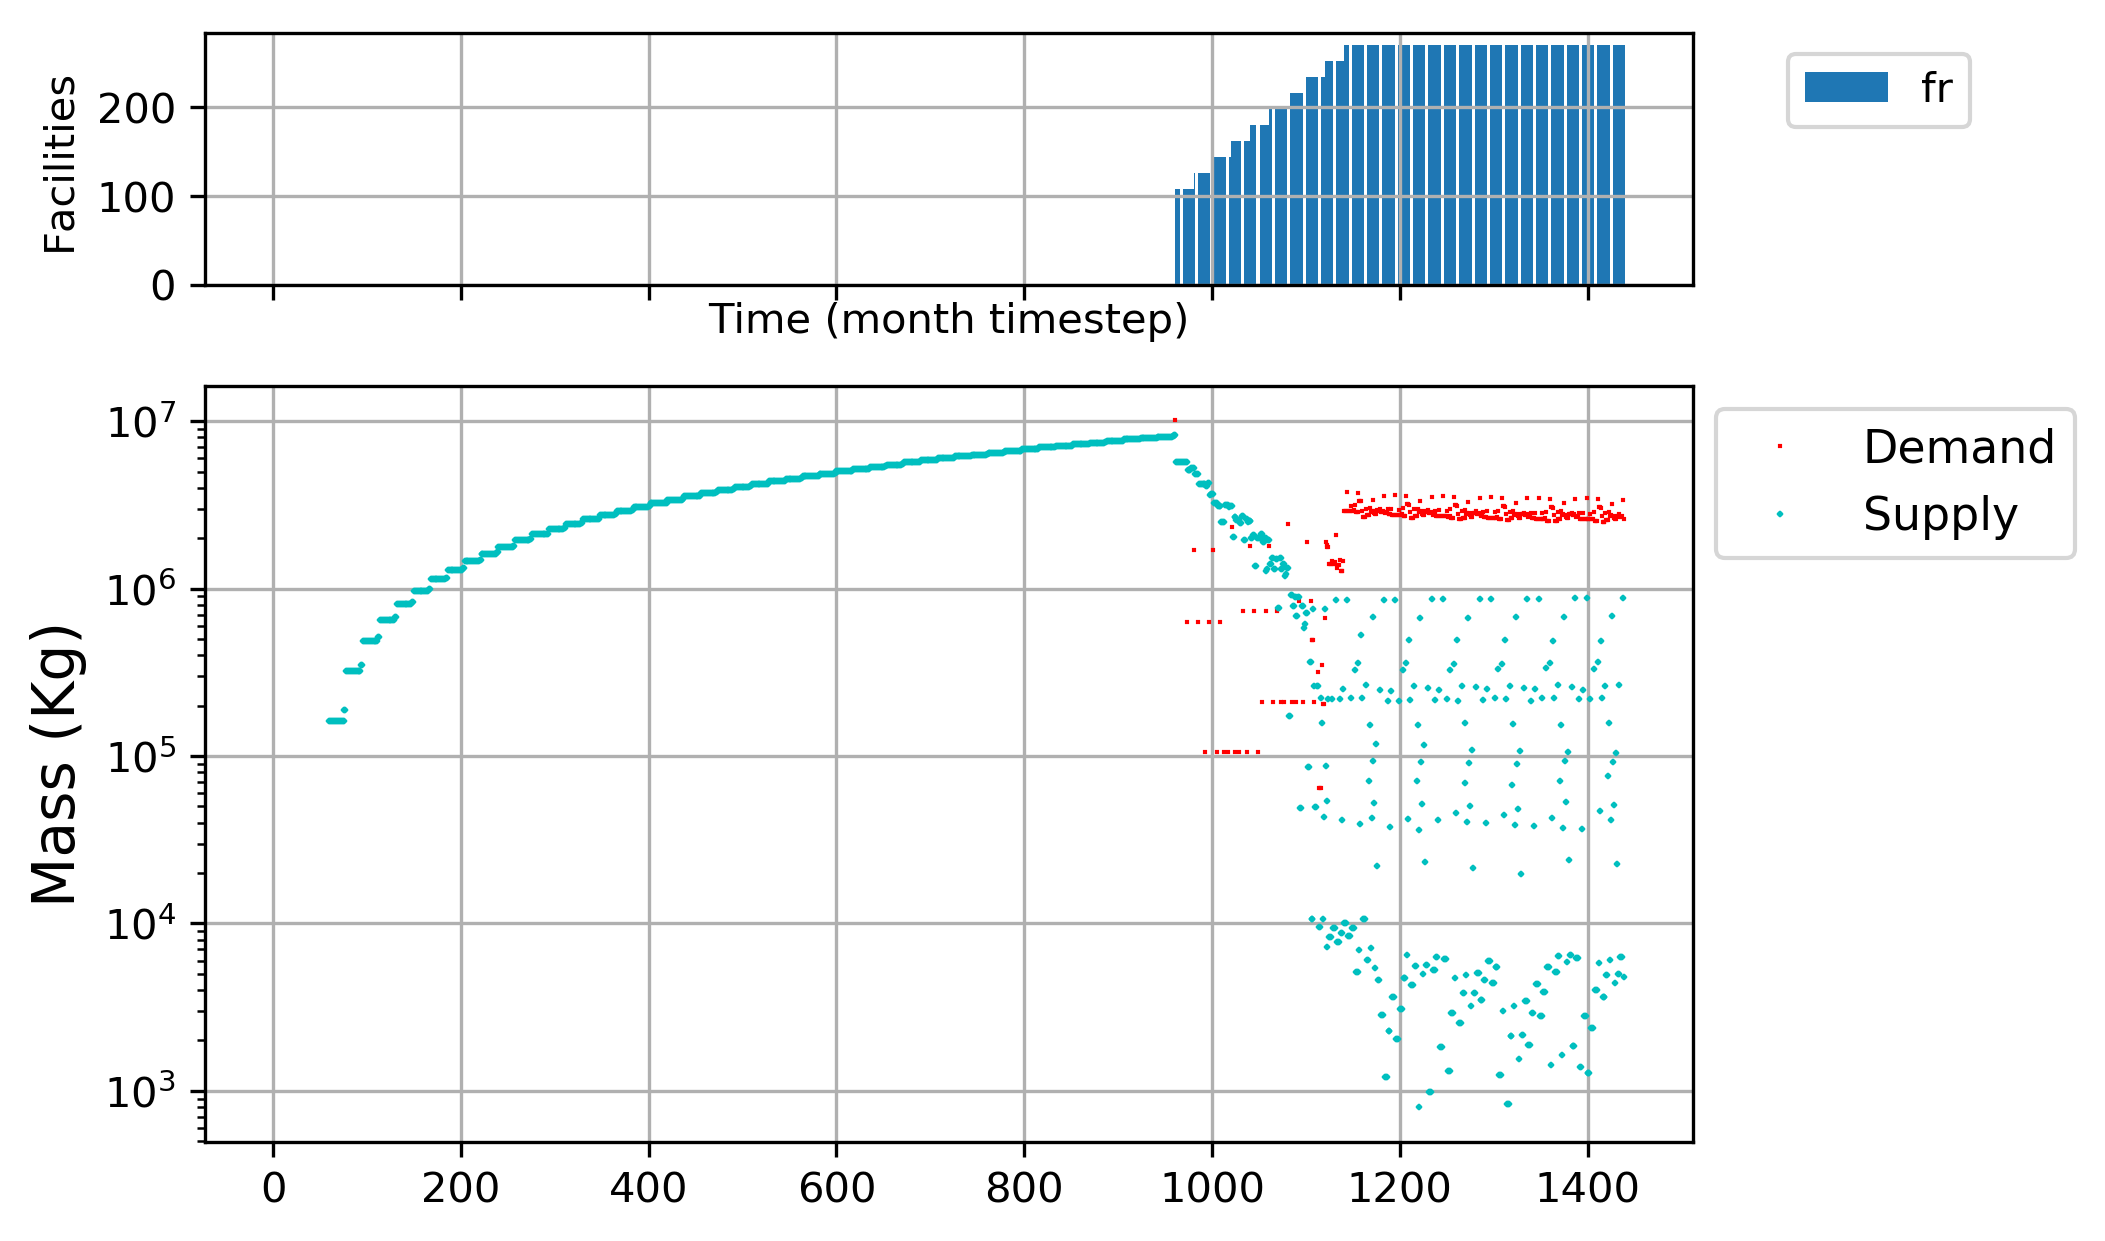
\includegraphics[width=\textwidth]{23-figures/0-poly-mixerout.png} 
	\hfill
	\caption{Demand and supply of FR fuel and number of FR reactors.}
	\label{fig:23-mixerout}
\end{figure}

\begin{figure}[H]
	\centering
	\begin{subfigure}[t]{0.45\textwidth}
		\centering
		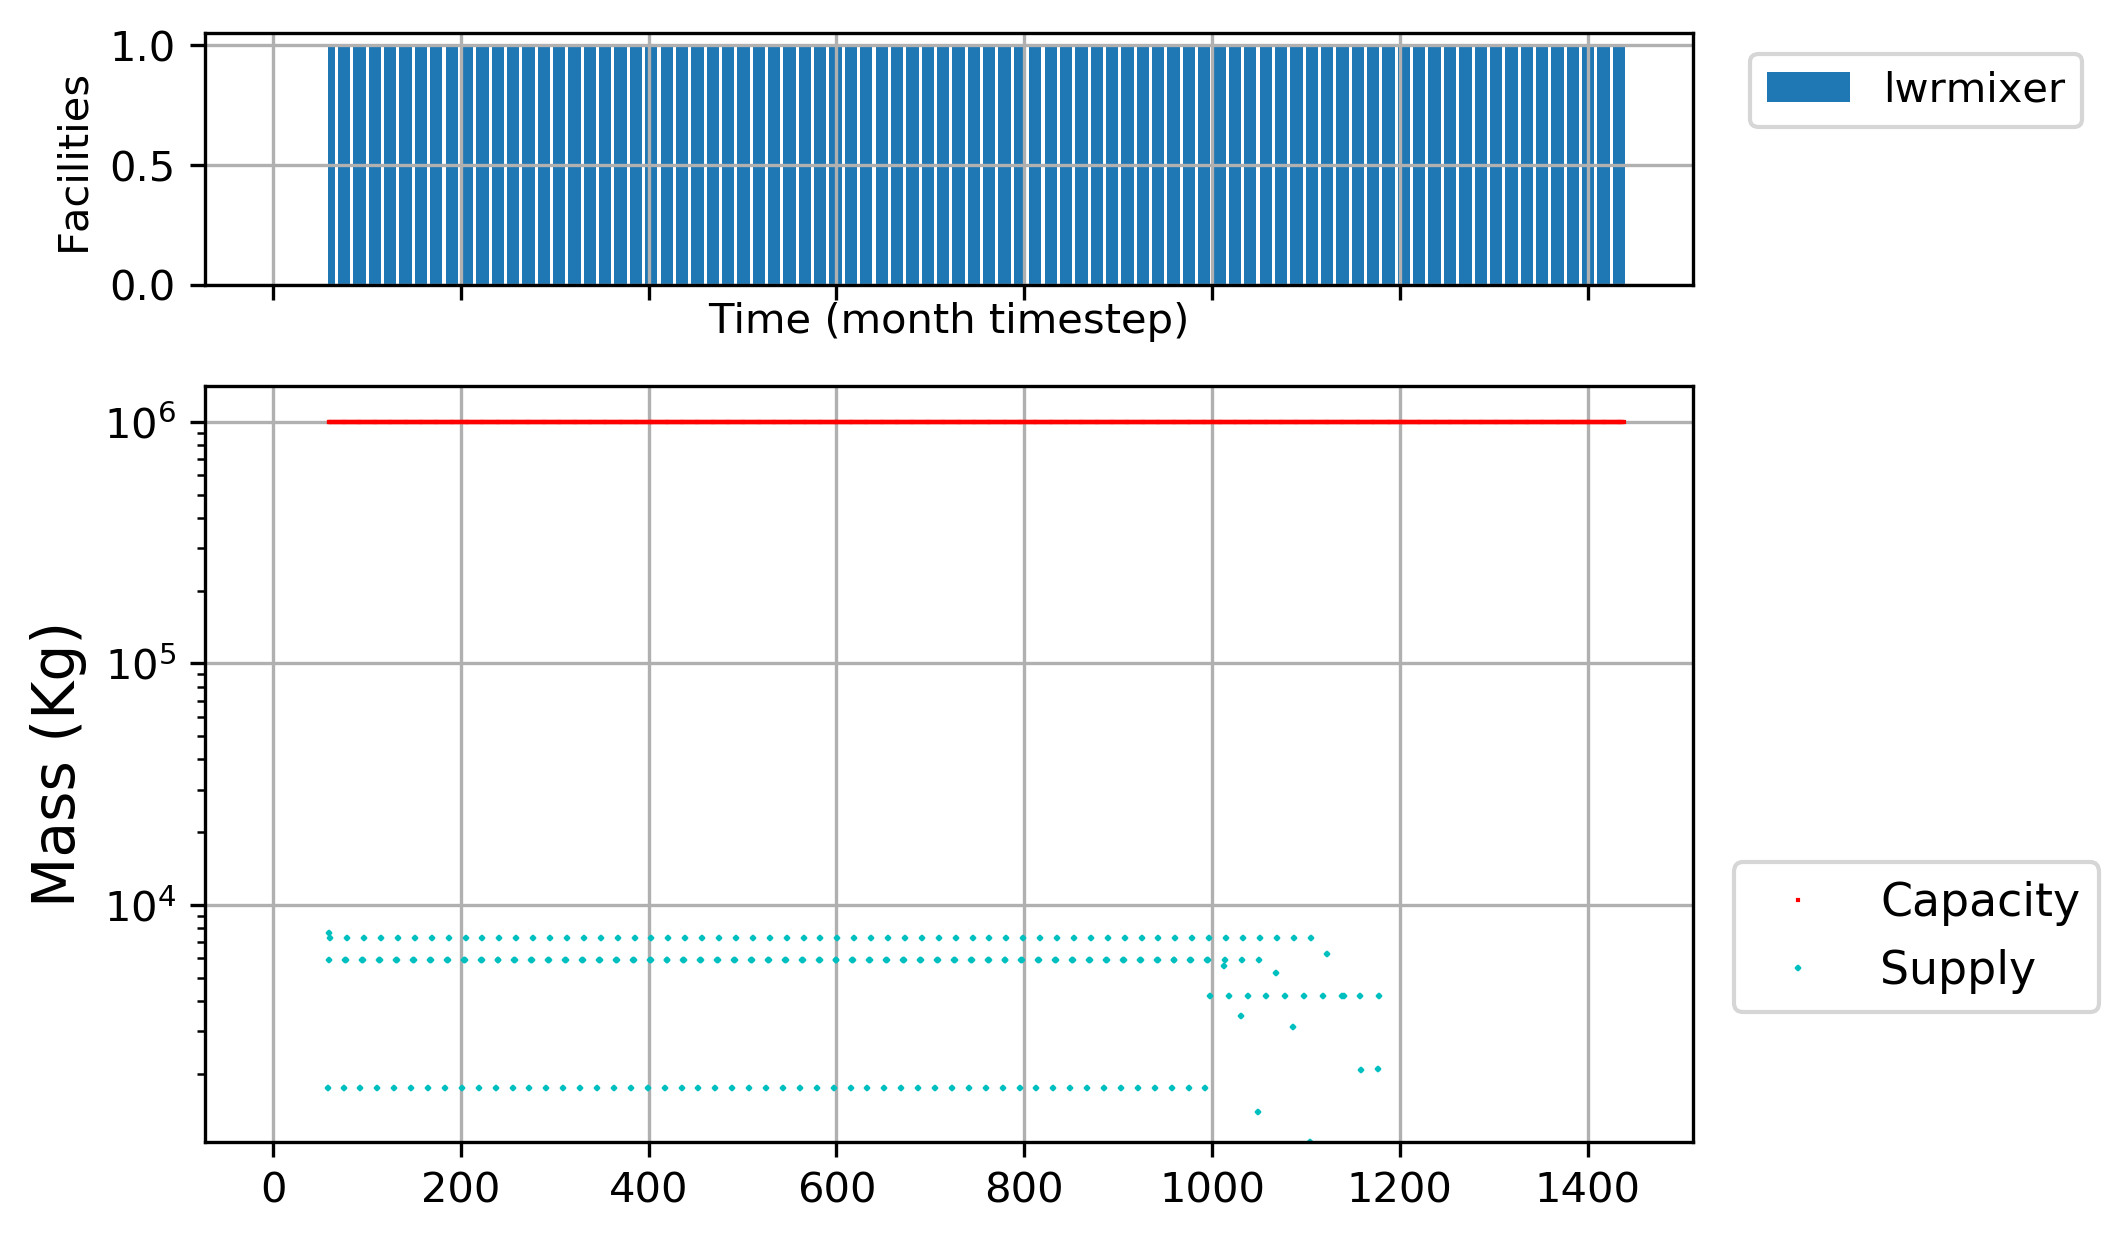
\includegraphics[width=\linewidth]{23-figures/0-poly-lwrpu.png} 
		\caption{Reprocessed Pu from spent fuel of LWRs.}
		\label{fig:23-lwrpu}
	\end{subfigure}
	\vspace{1cm}
	\begin{subfigure}[t]{0.45\textwidth}
		\centering
		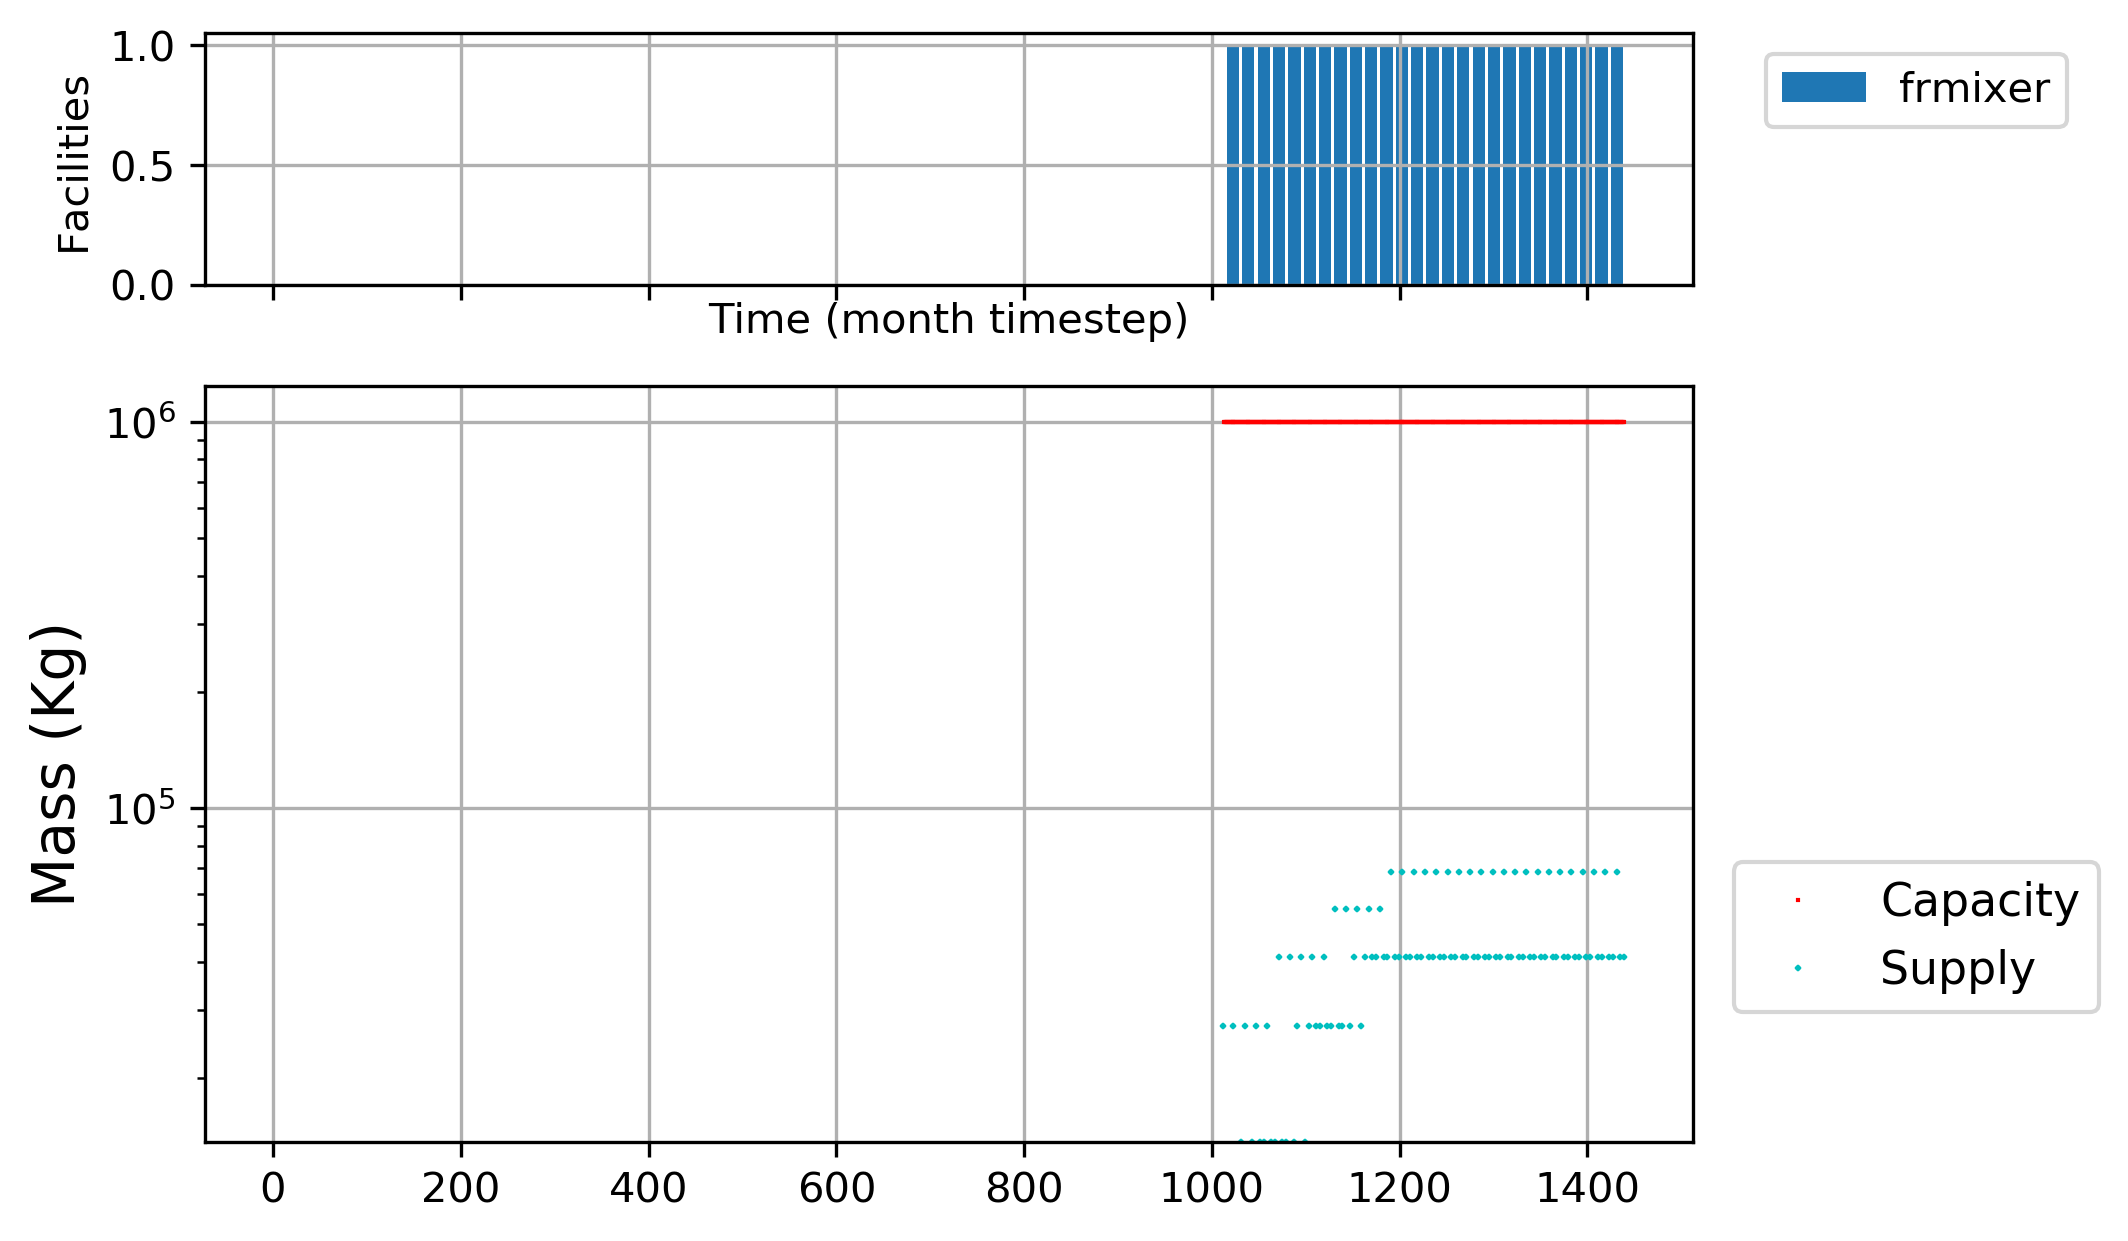
\includegraphics[width=\linewidth]{23-figures/0-poly-frpu.png} 
		\caption{Reprocessed Pu from spent fuel of FRs.}
		\label{fig:23-frpu}
	\end{subfigure}
	\hfill
	\caption{Demand and supply of different commodities and number of facilities supplied with them.}
	\label{fig:23-pu}
\end{figure}

\begin{table}[H]
	\centering
	\caption{Undersupply and oversupply of different commodities using poly to calculate EG01-EG23.}
	\label{tab:23-commod}
	\begin{tabularx}{\textwidth}{lRRR}
		\hline
		Commodity & Undersupplied & Cumulative  & Cumulative \\
		& Timesteps     & Undersupply [$10^3$Kg]  & Oversupply [$10^6$Kg] \\ \hline
		Natural-U & 2 & 4713  &  35648   \\ 
		Enriched-U & 4 & 48.5$\cdot10^3$  &  42259   \\ 
        \shortstack{Reprocessed Pu from \\ spent fuel of LWRs} & 1 & 1.7 & - \\
        \shortstack[l]{Reprocessed Pu from \\ spent fuel of FRs} & 1 & 27.4 & - \\ \hline
	\end{tabularx}
\end{table}

\section{Eg01-Eg24}

Figure \ref{fig:24flow} shows the facility and mass flow of transition scenario 
Eg01-Eg24 in \Cyclus.

\begin{figure}[H]
	\centering
	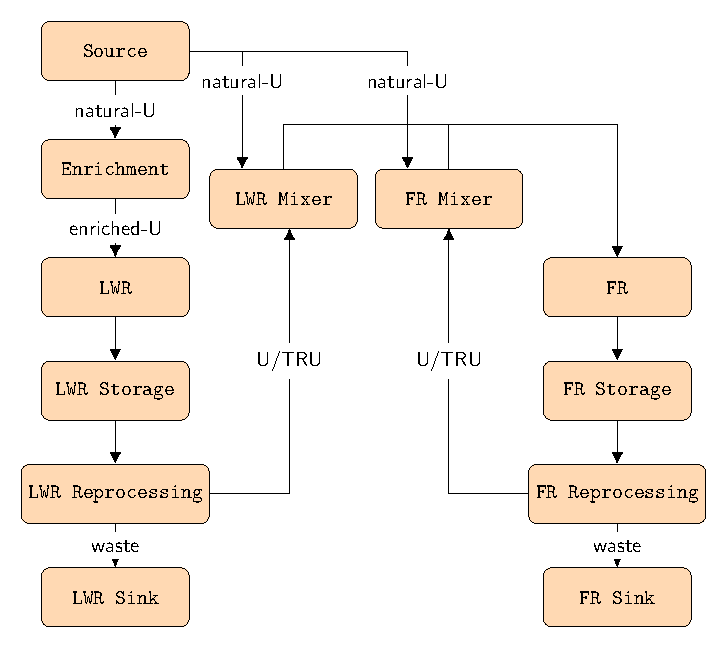
\includegraphics[width=0.9\textwidth]{24-figures/24flow.pdf} 
	\hfill
	\caption{Diagram with facilities and mass flow of the scenario EG01-EG24.}
	\label{fig:24flow}
\end{figure}

\subsection{Linearly increasing Power Demand: Power}

This section presents plots of power for all the prediction methods. 
The power demand increases linearly with the expression $60000 + 250t/12 MW$. 
Table \ref{tab:24-inputs} shows the input parameters. 
Figures \ref{fig:24-lin-NO}, \ref{fig:24-lin-DO}, and \ref{fig:24-lin-SO} 
display the power demand and corresponding supply for the Non-optimizing (NO), 
Deterministic-optimizing (DO), and Stochastic-optimizing methods (SO), respectively. 
The plots only show the power demand and supply during the transition period. 
Undersupply of power occur during two main time periods:  
initial demand for the commodity and during the transition period. 
Undersupply time steps occurring at the beginning of the simulation 
is expected since without time series data at the beginning of the simulation, 
\deploy takes a few time steps to collect time series data about power demand 
to begin predicting and starting deployment of reactor and supporting fuel 
cycle facilities. 
Table \ref{tab:24-lin-power} records the number of steps of undersupply, 
the cumulative undersupply, and the cumulative oversupply. 
The smallest cumulative undersupply and smallest amount of undersupply 
time steps are for the fft prediction method.

\begin{table}[H]
	\centering
	\caption{EG01-EG24 input file values.}
	\label{tab:24-inputs}
	\begin{tabularx}{\textwidth}{lR}
		\hline
		Parameter			& Input \\ 	\hline
		Demand equation [MW]		& $60000 + 250t/12 MW$  \\
		Deployment Driving Method 	& Installed Capacity \\
		Power Buffer [MW]   			& 0 \\
		Forward Steps		& 1 \\
		Backward Steps		& 2 \\		\hline
	\end{tabularx}
\end{table}

\begin{figure}[H]
	\centering
	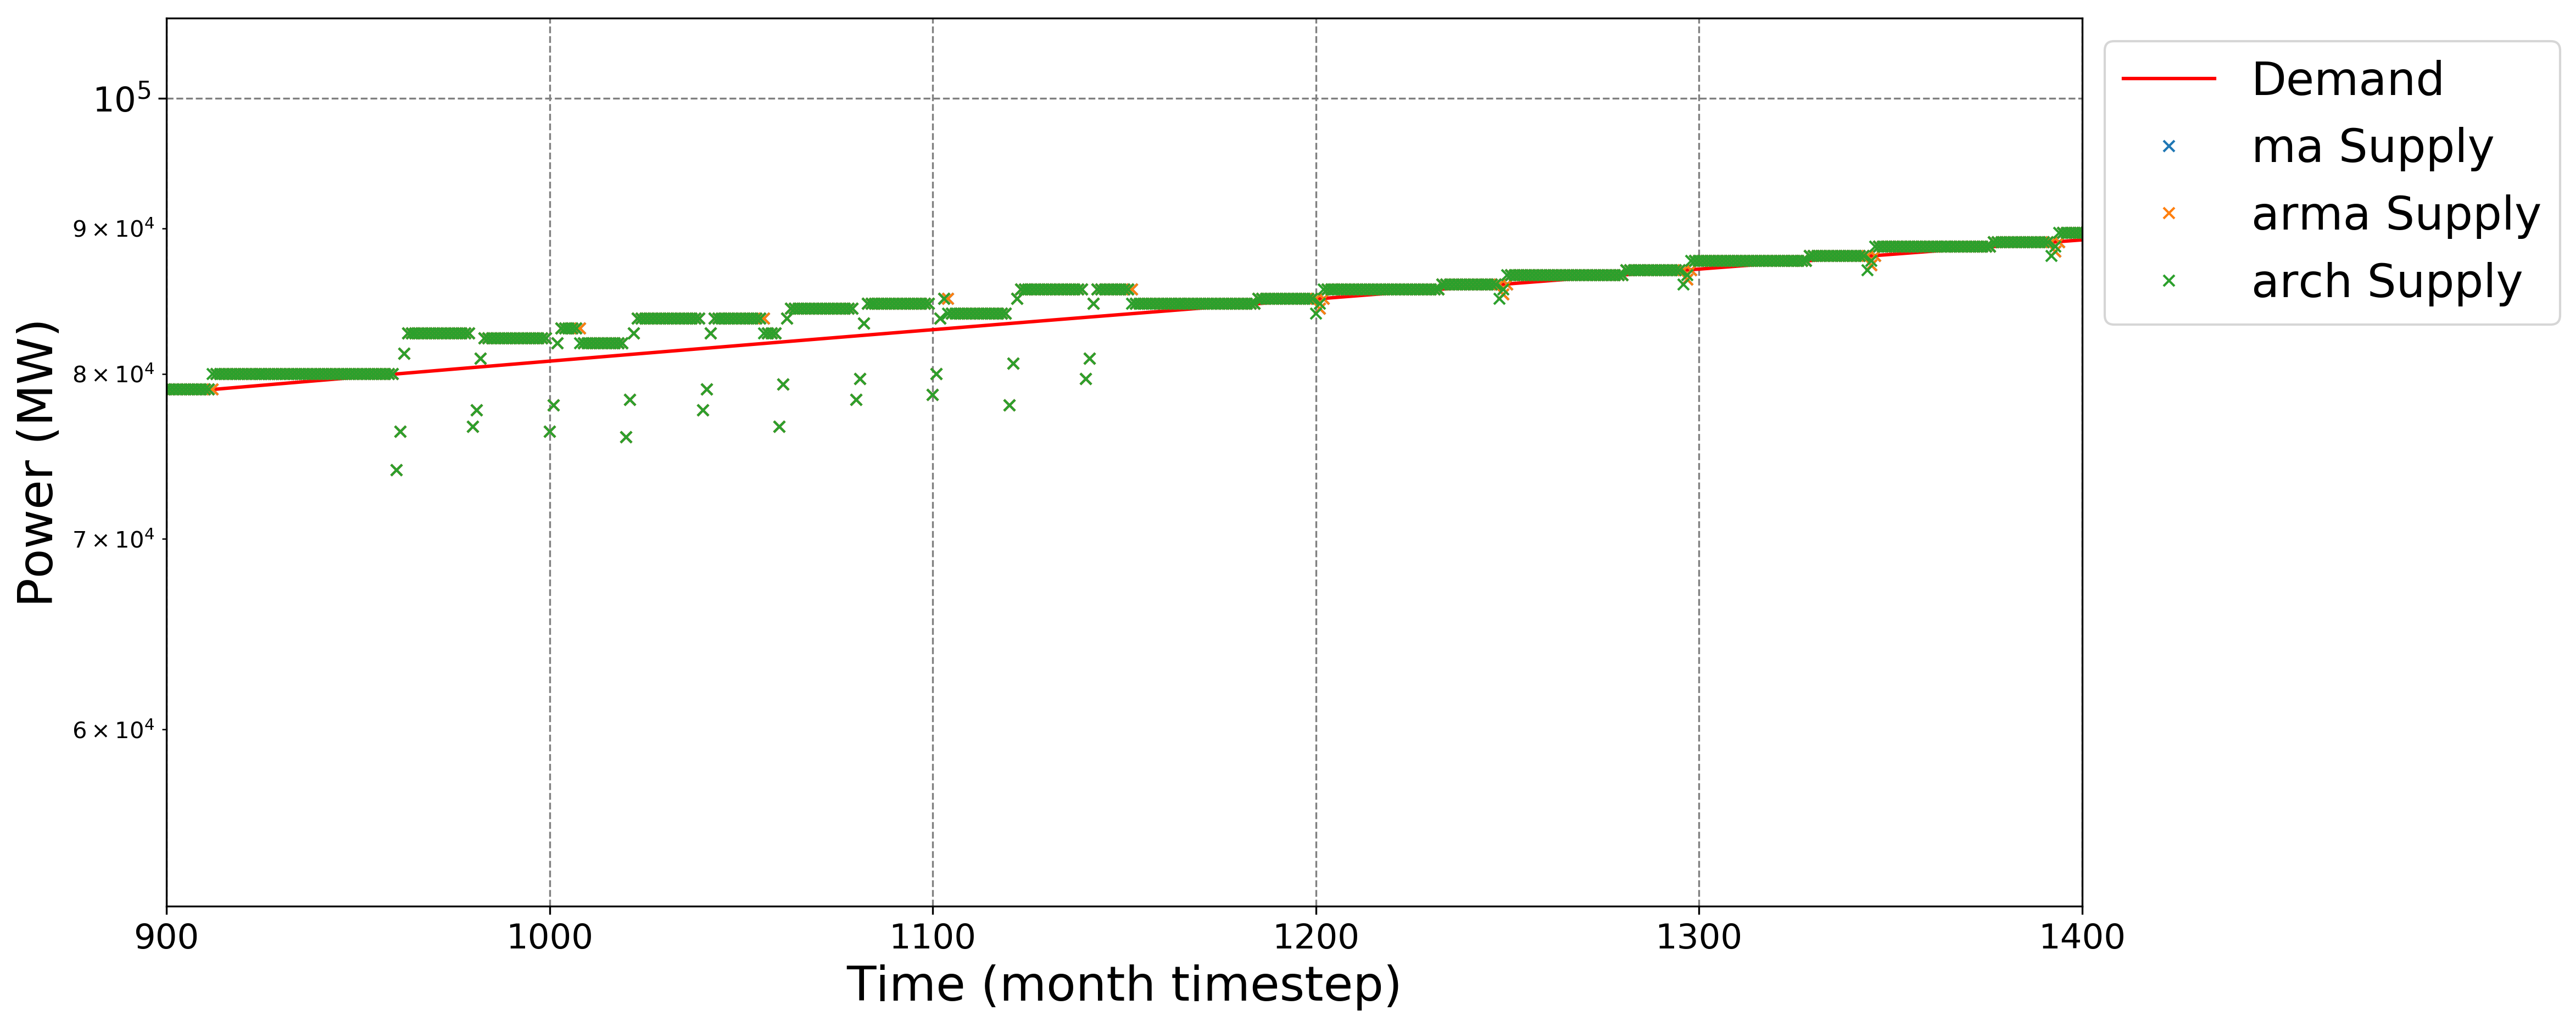
\includegraphics[width=\textwidth]{24-figures/lin-24-power-buffer01.png} 
	\hfill
	\caption{Linearly increasing power demand ($60000 + 250t/12 MW$) and power supply obtained 
	with the NO algorithms.}
	\label{fig:24-lin-NO}
\end{figure}

\begin{figure}[H]
	\centering
	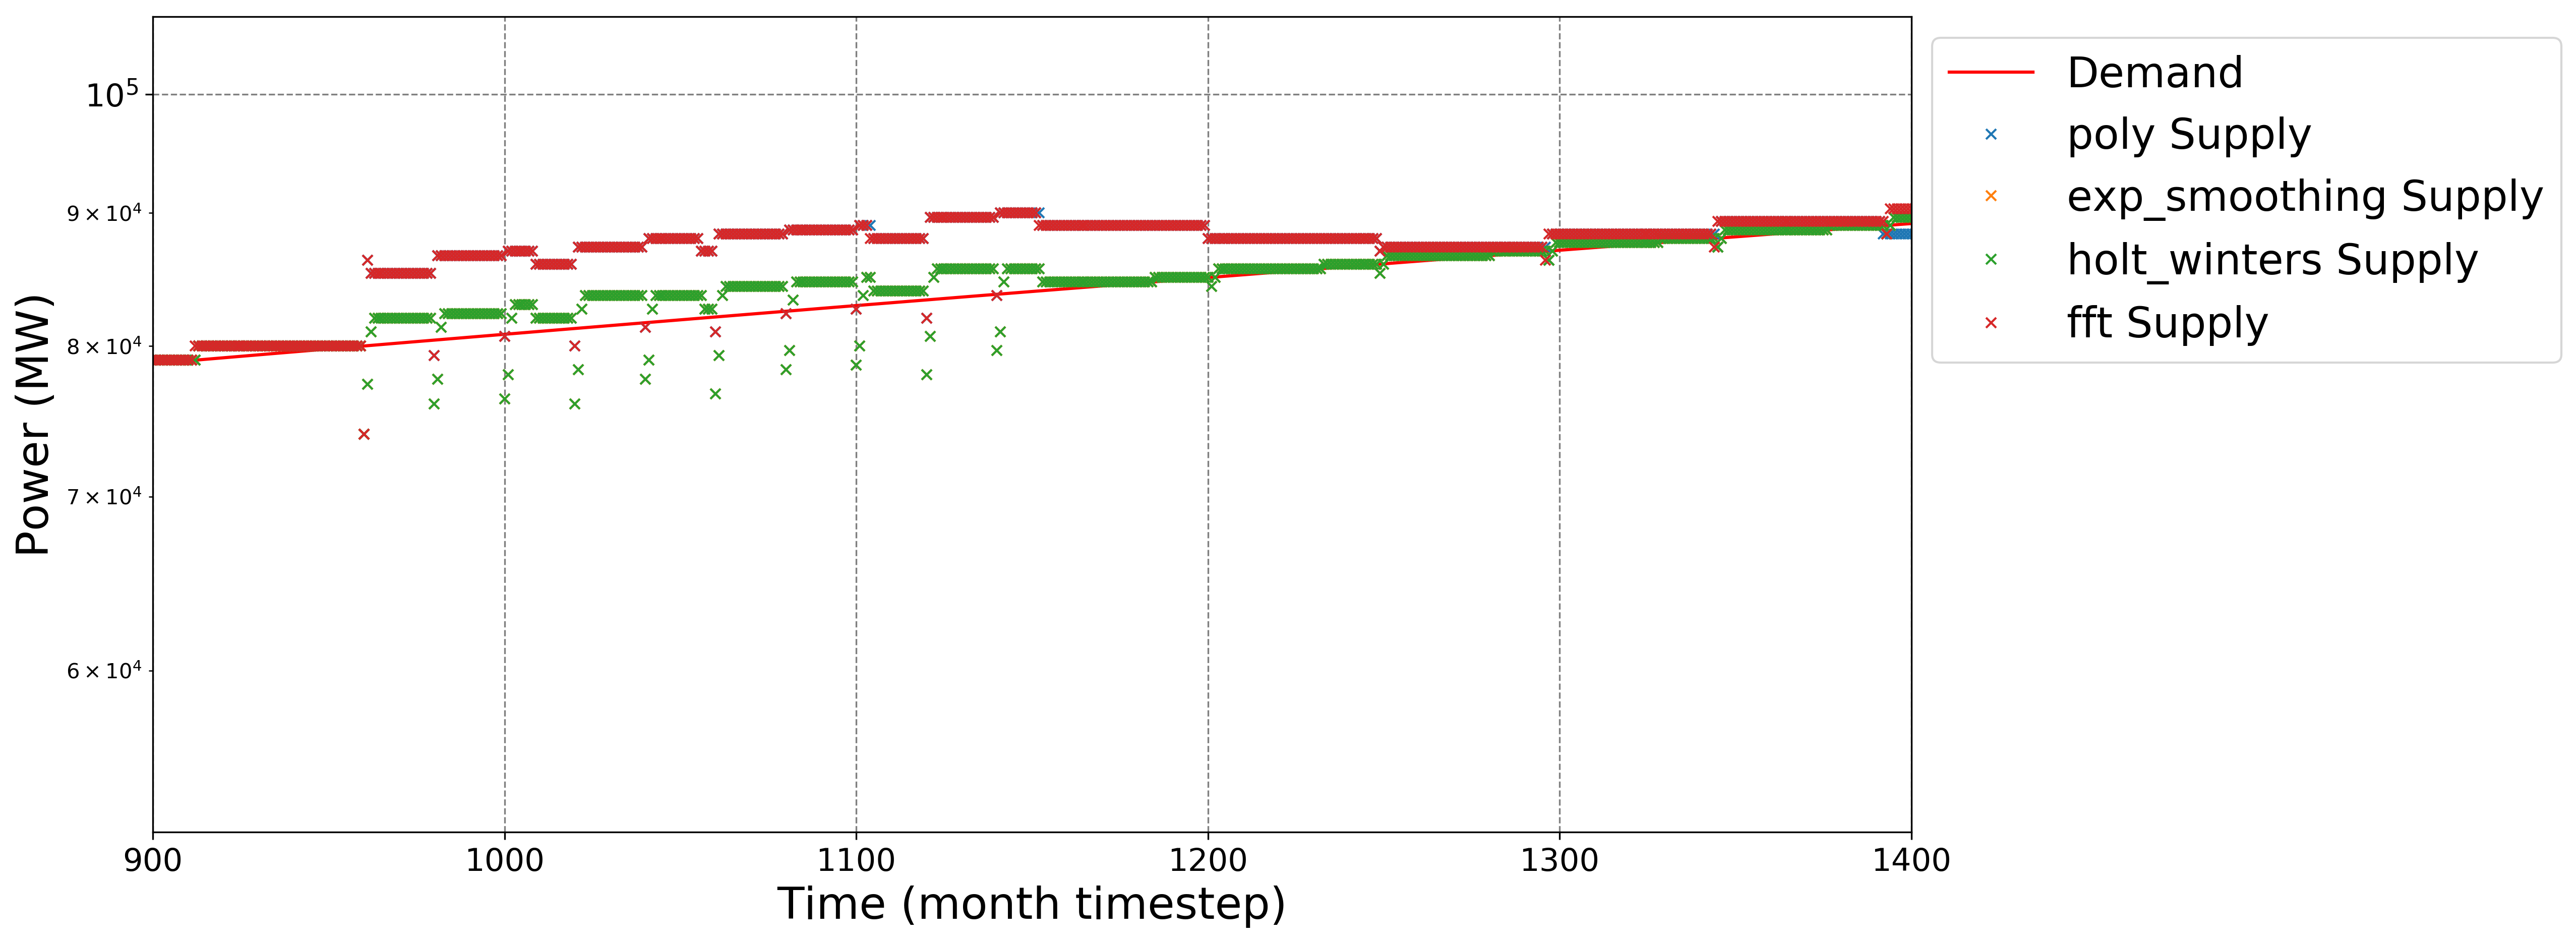
\includegraphics[width=\textwidth]{24-figures/lin-24-power-buffer02.png} 
	\hfill
	\caption{Linearly increasing power demand ($60000 + 250t/12 MW$) and power supply obtained 
	with the DO algorithms.}
	\label{fig:24-lin-DO}
\end{figure}

\begin{figure}[H]
	\centering
	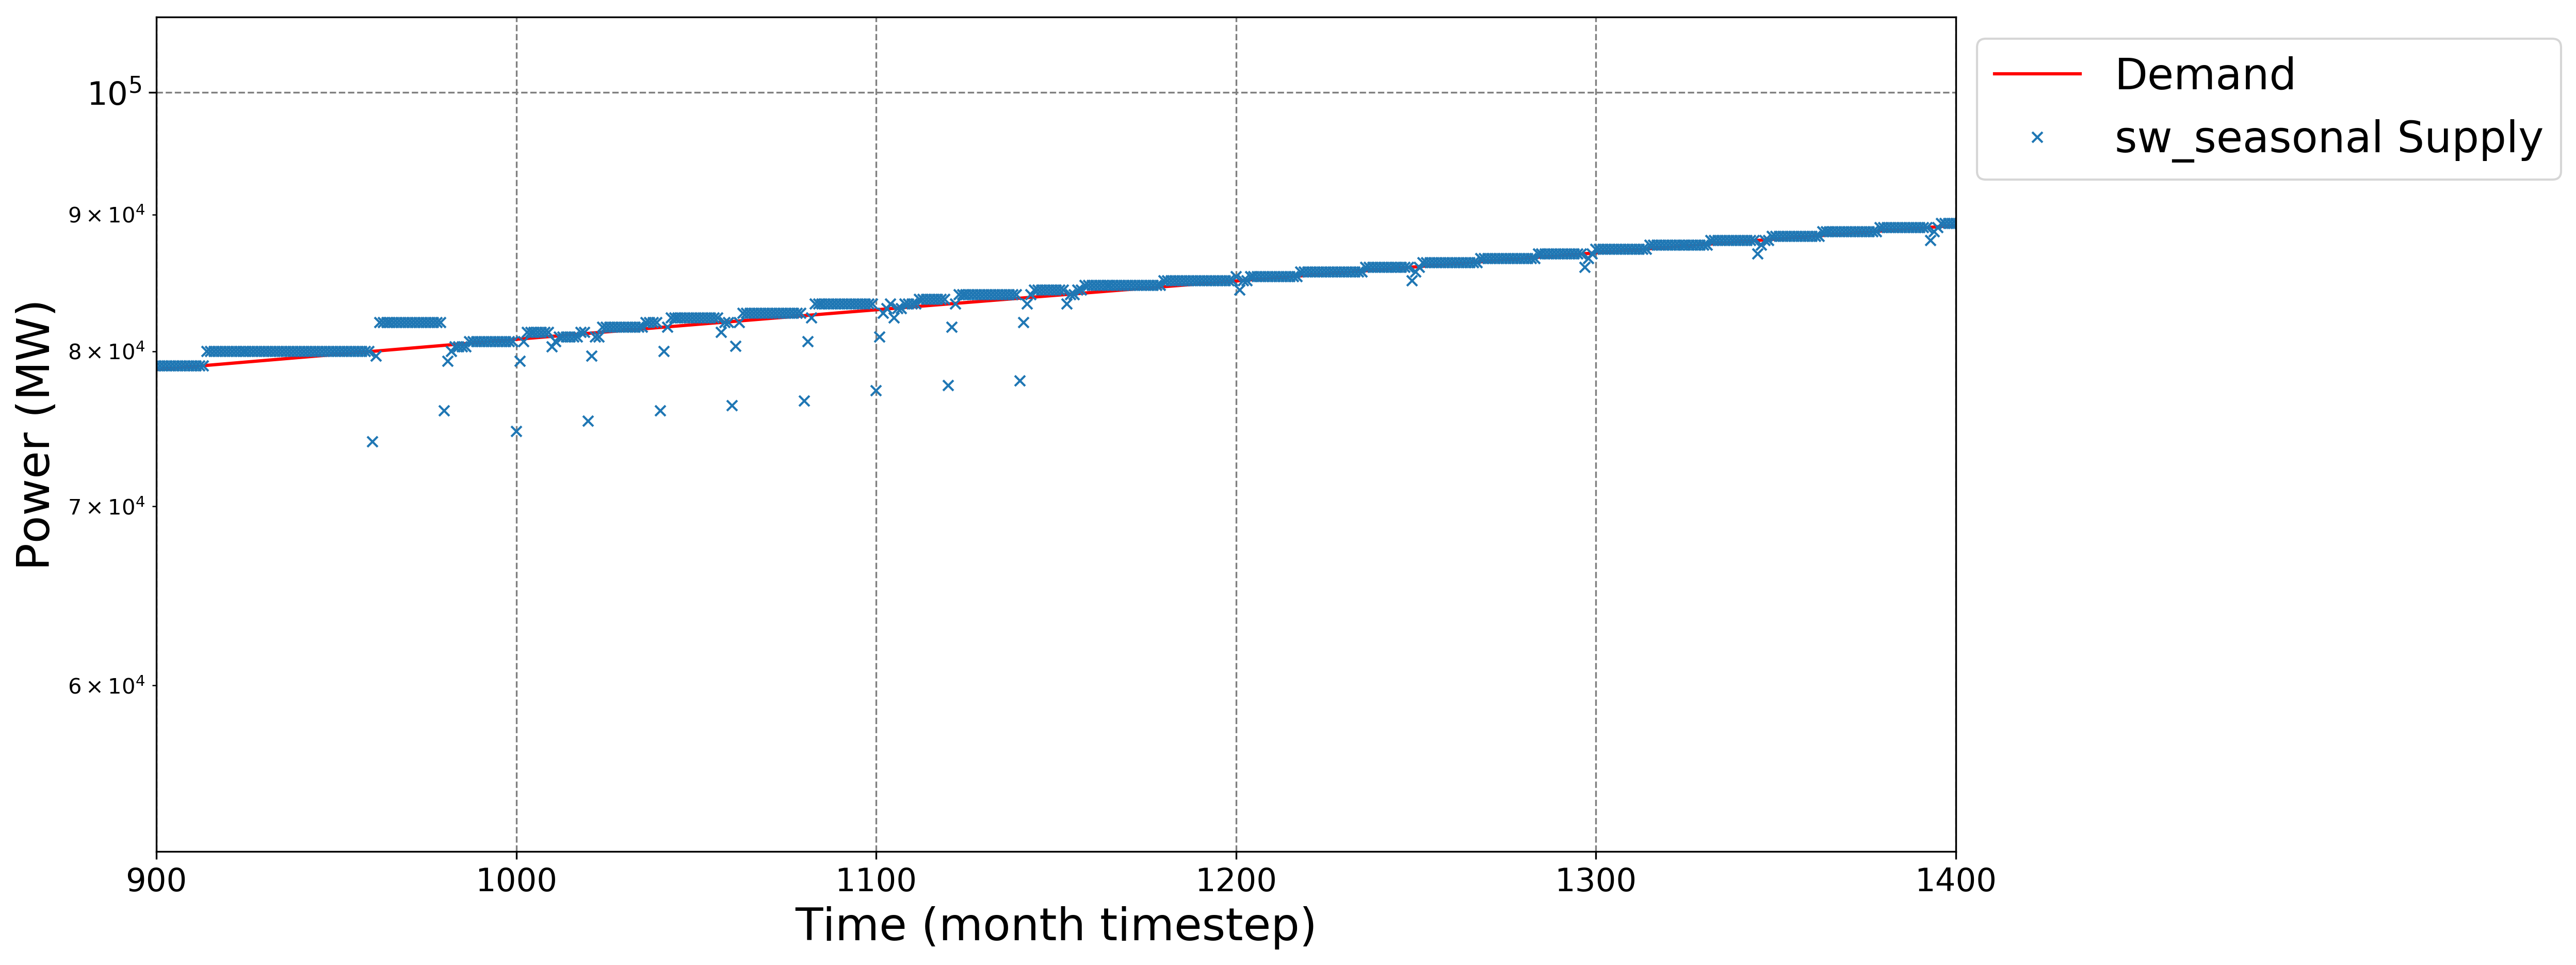
\includegraphics[width=\textwidth]{24-figures/lin-24-power-buffer03.png} 
	\hfill
	\caption{Linearly increasing power demand ($60000 + 250t/12 MW$) and power supply obtained with the SO algorithms.}
	\label{fig:24-lin-SO}
\end{figure}

\begin{table}[H]
	\centering
	\caption{Undersupply and oversupply of Power for the different prediction algorithms used to calculate EG01-EG24.}
	\label{tab:24-lin-power}
	\begin{tabularx}{\textwidth}{lRRR}
		\hline
		Algorithm & Undersupplied & Cumulative  & Cumulative \\
		& Timesteps     & Undersupply [GW.mo]  & Oversupply [GW.mo] \\ \hline
		MA        & 36 	& 313.7 & 840.9 \\ 
		ARMA      & 36 	& 313.7 & 840.9 \\ 
		ARCH      & 36 	& 316.8 & 859.0 \\ 
		POLY      &  65 & 282.4 & 1974.7 \\ 
		EXP\_SMOOTHING 	& 37 & 373.4 & 828.7 \\ 
		HOLT-WINTERS  	& 37 & 373.4 & 828.7 \\ 
		FFT       & 20	& 315.1	& 2019.1 \\ 
		SW\_SEASONAL    & 107 & 318.8 & 579.09 \\ \hline
	\end{tabularx}
\end{table}

\subsection{Buffer}

This section presents a sensitivity analysis for varying power buffer values. 
Figure \ref{fig:24-buff} shows a comparison of the cumulative undersupply 
for different buffer sizes using the fft prediction method. 
Figure \ref{fig:24-buf-fft} displays the power demand and supply for different 
values of the buffer using fft. 
The cumulative undersupply decreases with the increasing values of the buffer until it  
reaches an asymptotic value. 
That value is due to the undersupply at the beginning of the scenario, when the buffer size 
does not considerably impact the undersupply.

\begin{figure}[H]
	\centering
	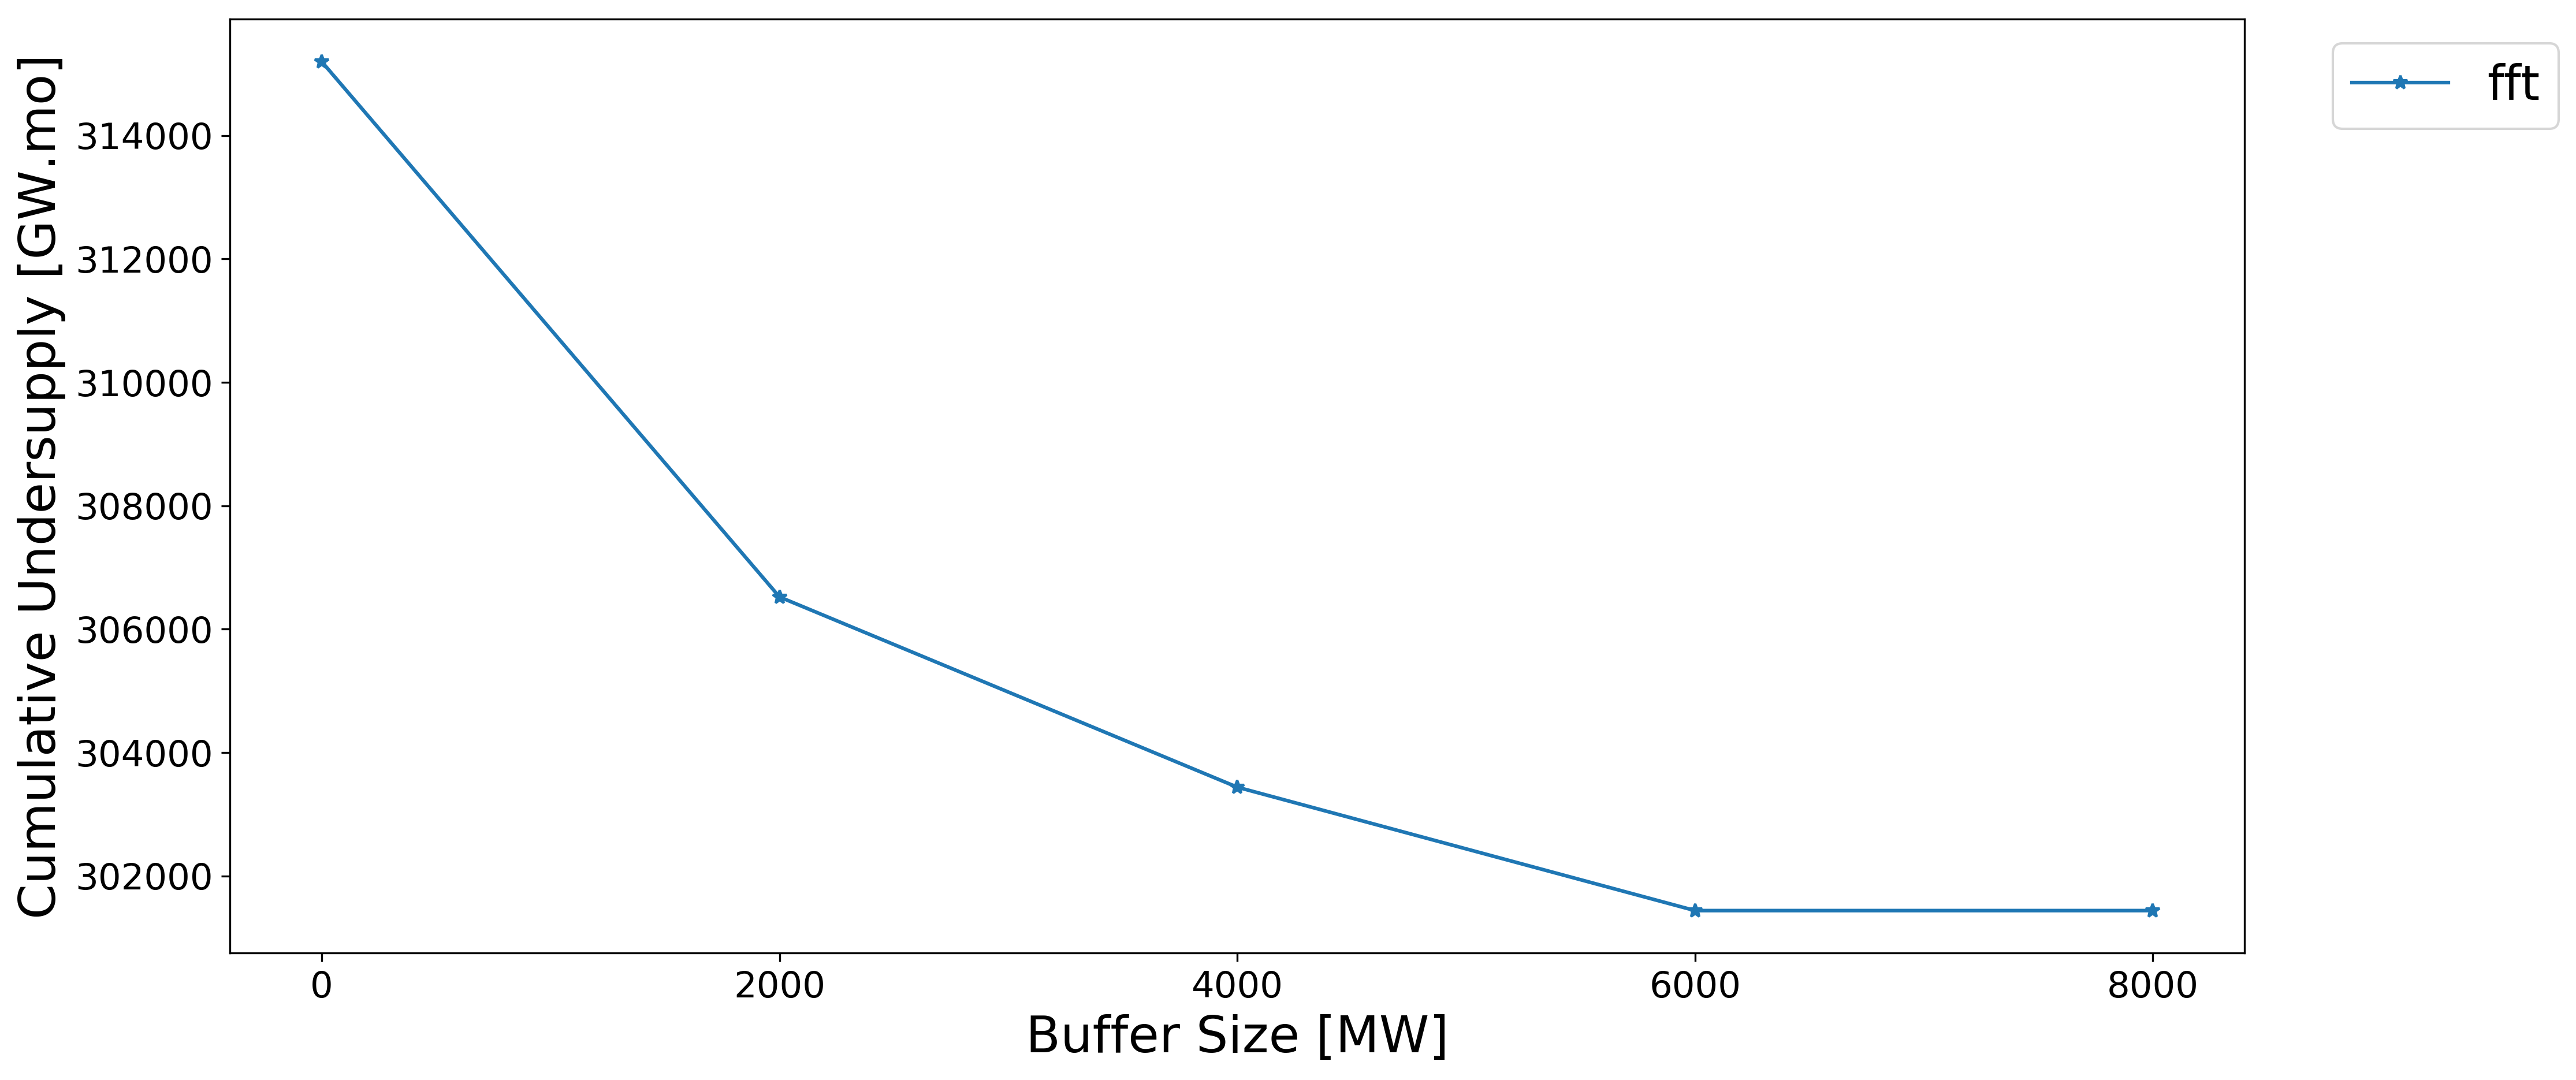
\includegraphics[width=\textwidth]{24-figures/24-sens-buffer.png} 
	\hfill
	\caption{Sensitivity analysis for different buffer sizes using the fft prediction method.}
	\label{fig:24-buff}
\end{figure}

\begin{figure}[H]
	\centering
	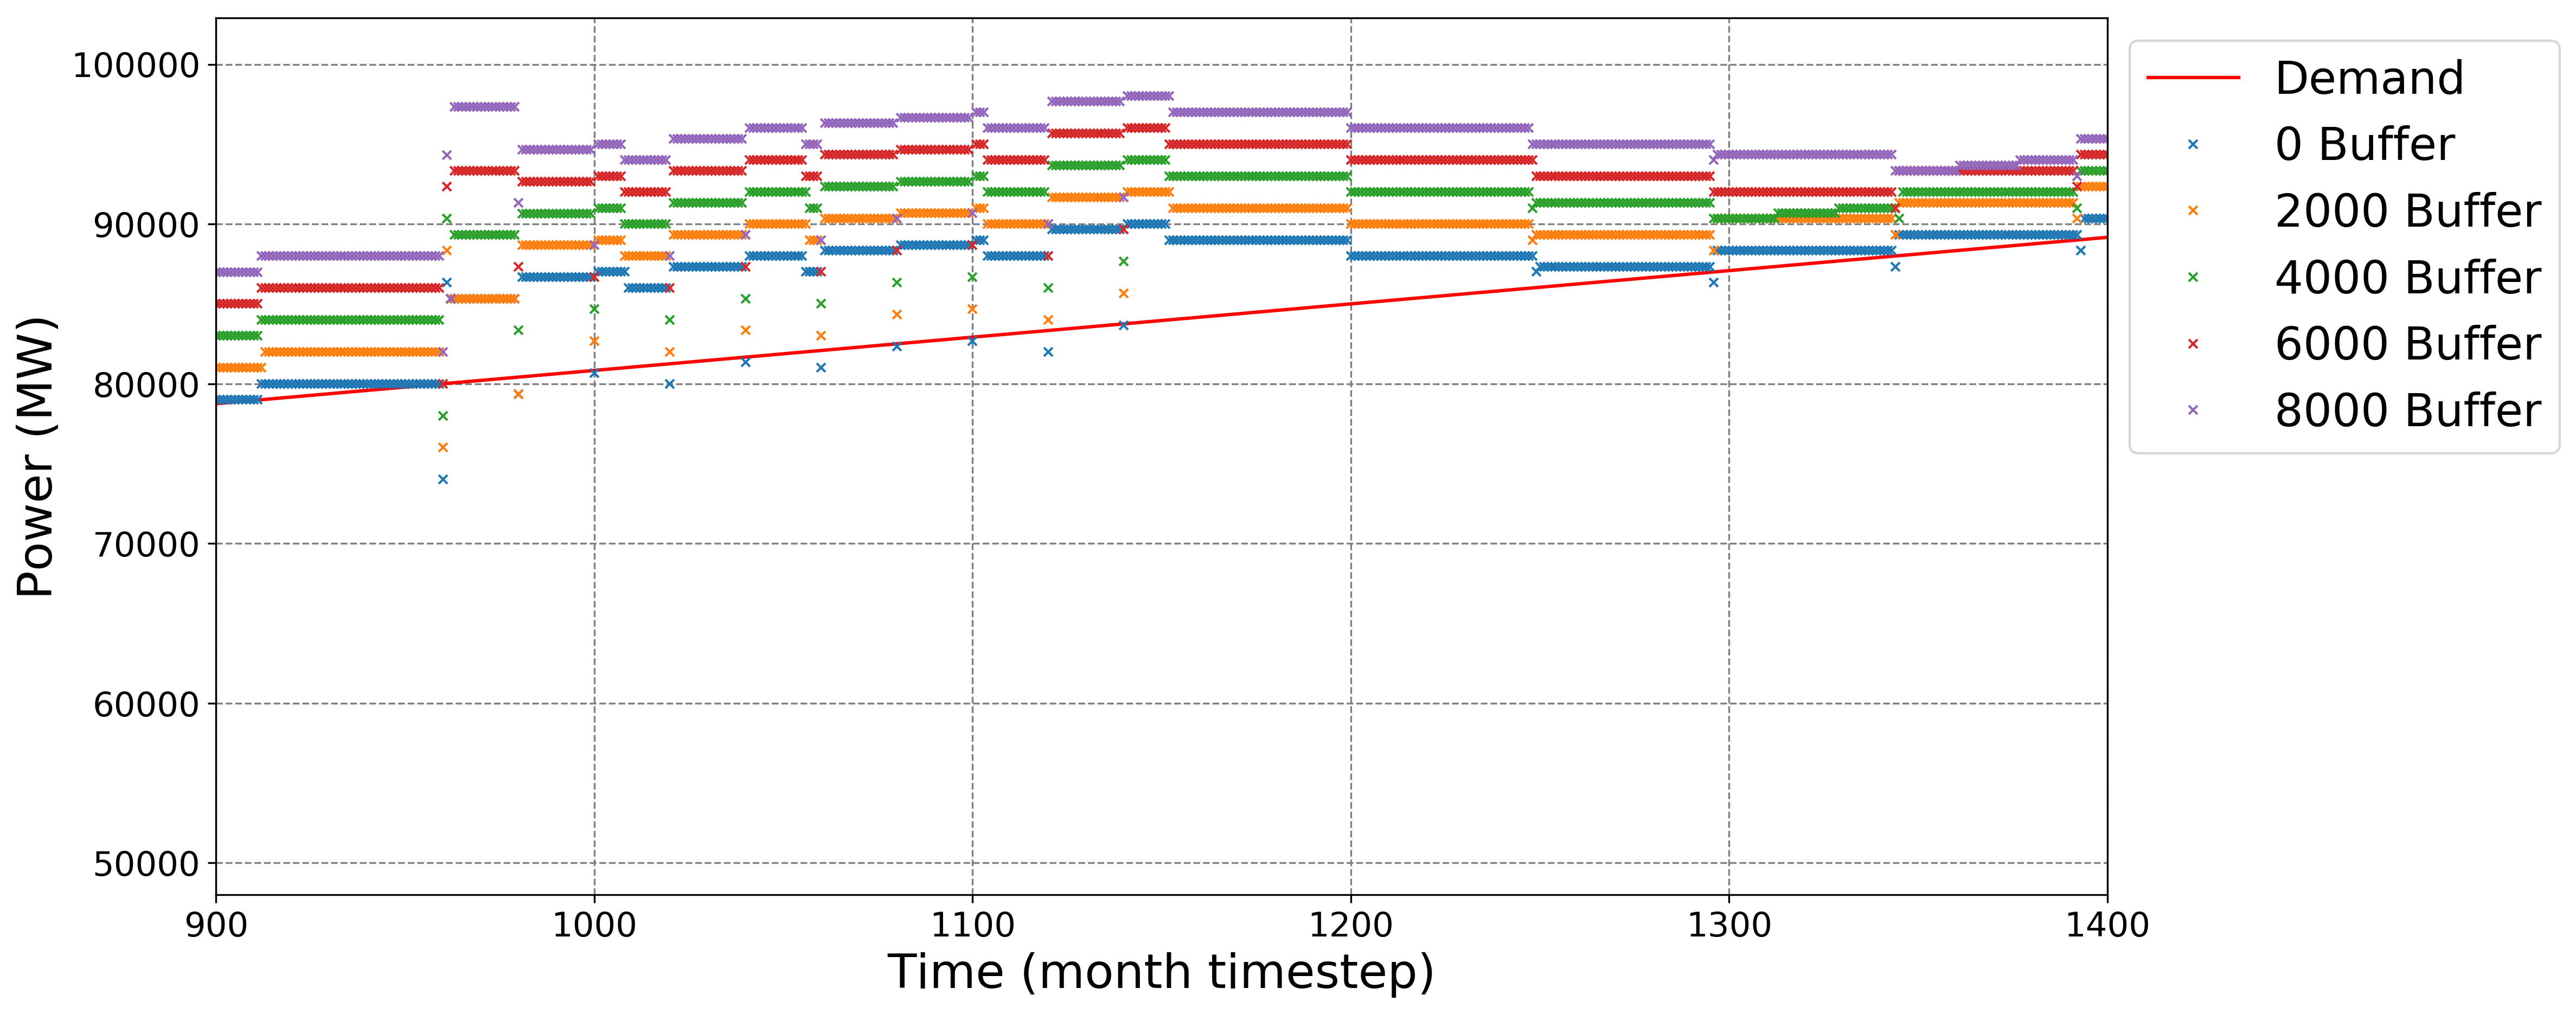
\includegraphics[width=\textwidth]{24-figures/24-power-buffer-fft.png} 
	\hfill
	\caption{Power supply for different buffer sizes using the fft prediction method.}
	\label{fig:24-buf-fft}
\end{figure}

\section{Eg01-Eg29}

Figure \ref{fig:29flow} shows the facility and mass flow of transition scenario 
Eg01-Eg29 in \Cyclus.

\begin{figure}[H]
	\centering
	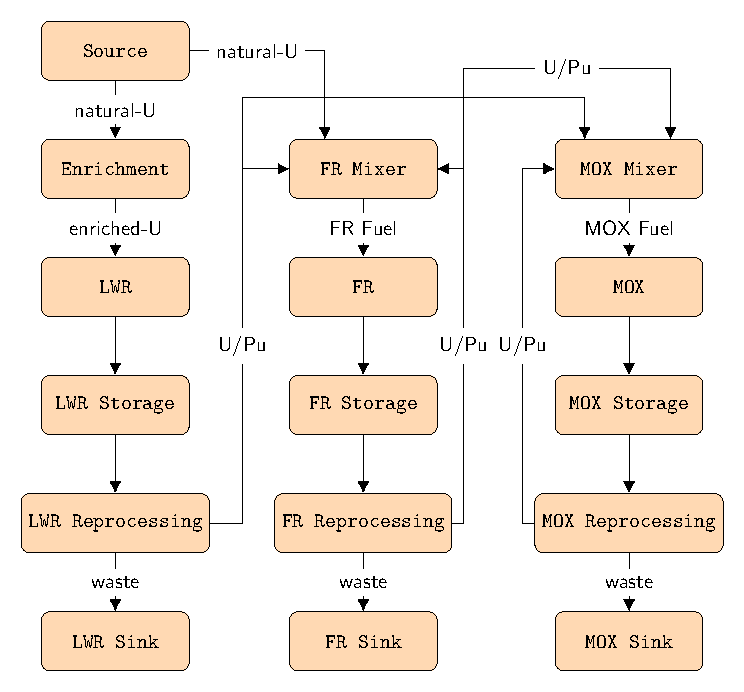
\includegraphics[width=\textwidth]{29-figures/29flow.pdf} 
	\hfill
	\caption{Diagram with facilities and mass flow of the scenario EG01-EG29.}
	\label{fig:29flow}
\end{figure}

\subsection{Flat Power Demand: Power}

This section presents plots of power for all the prediction methods. 
The power demand is 60000 MW throughout the simulation. 
Table \ref{tab:29-inputs} shows the input parameters. 
Figures \ref{fig:29-NO}, \ref{fig:29-DO}, and \ref{fig:29-SO} display 
the power demand supply for the Non-optimizing (NO), Deterministic-optimizing (DO), 
and Stochastic-optimizing methods (SO), respectively.
Table \ref{tab:29-power} records the number of steps with undersupply, 
the cumulative undersupply, and the cumulative oversupply. 
The smallest cumulative undersupply and smallest amount of undersupply 
time steps are for poly and fft prediction methods. 

\begin{table}[H]
	\centering
	\caption{EG01-EG29 input file values.}
	\label{tab:29-inputs}
	\begin{tabularx}{\textwidth}{lR}
		\hline
		Parameter			& Input \\ 	\hline
		Demand equation [GW]		& 60  \\
		Deployment Driving Method 	& Installed Capacity \\
		Power Buffer [MW]    			& 0 \\
		Forward Steps		& 1 \\
		Backward Steps		& 2 \\		\hline
	\end{tabularx}
\end{table}

\begin{figure}[H]
	\centering
	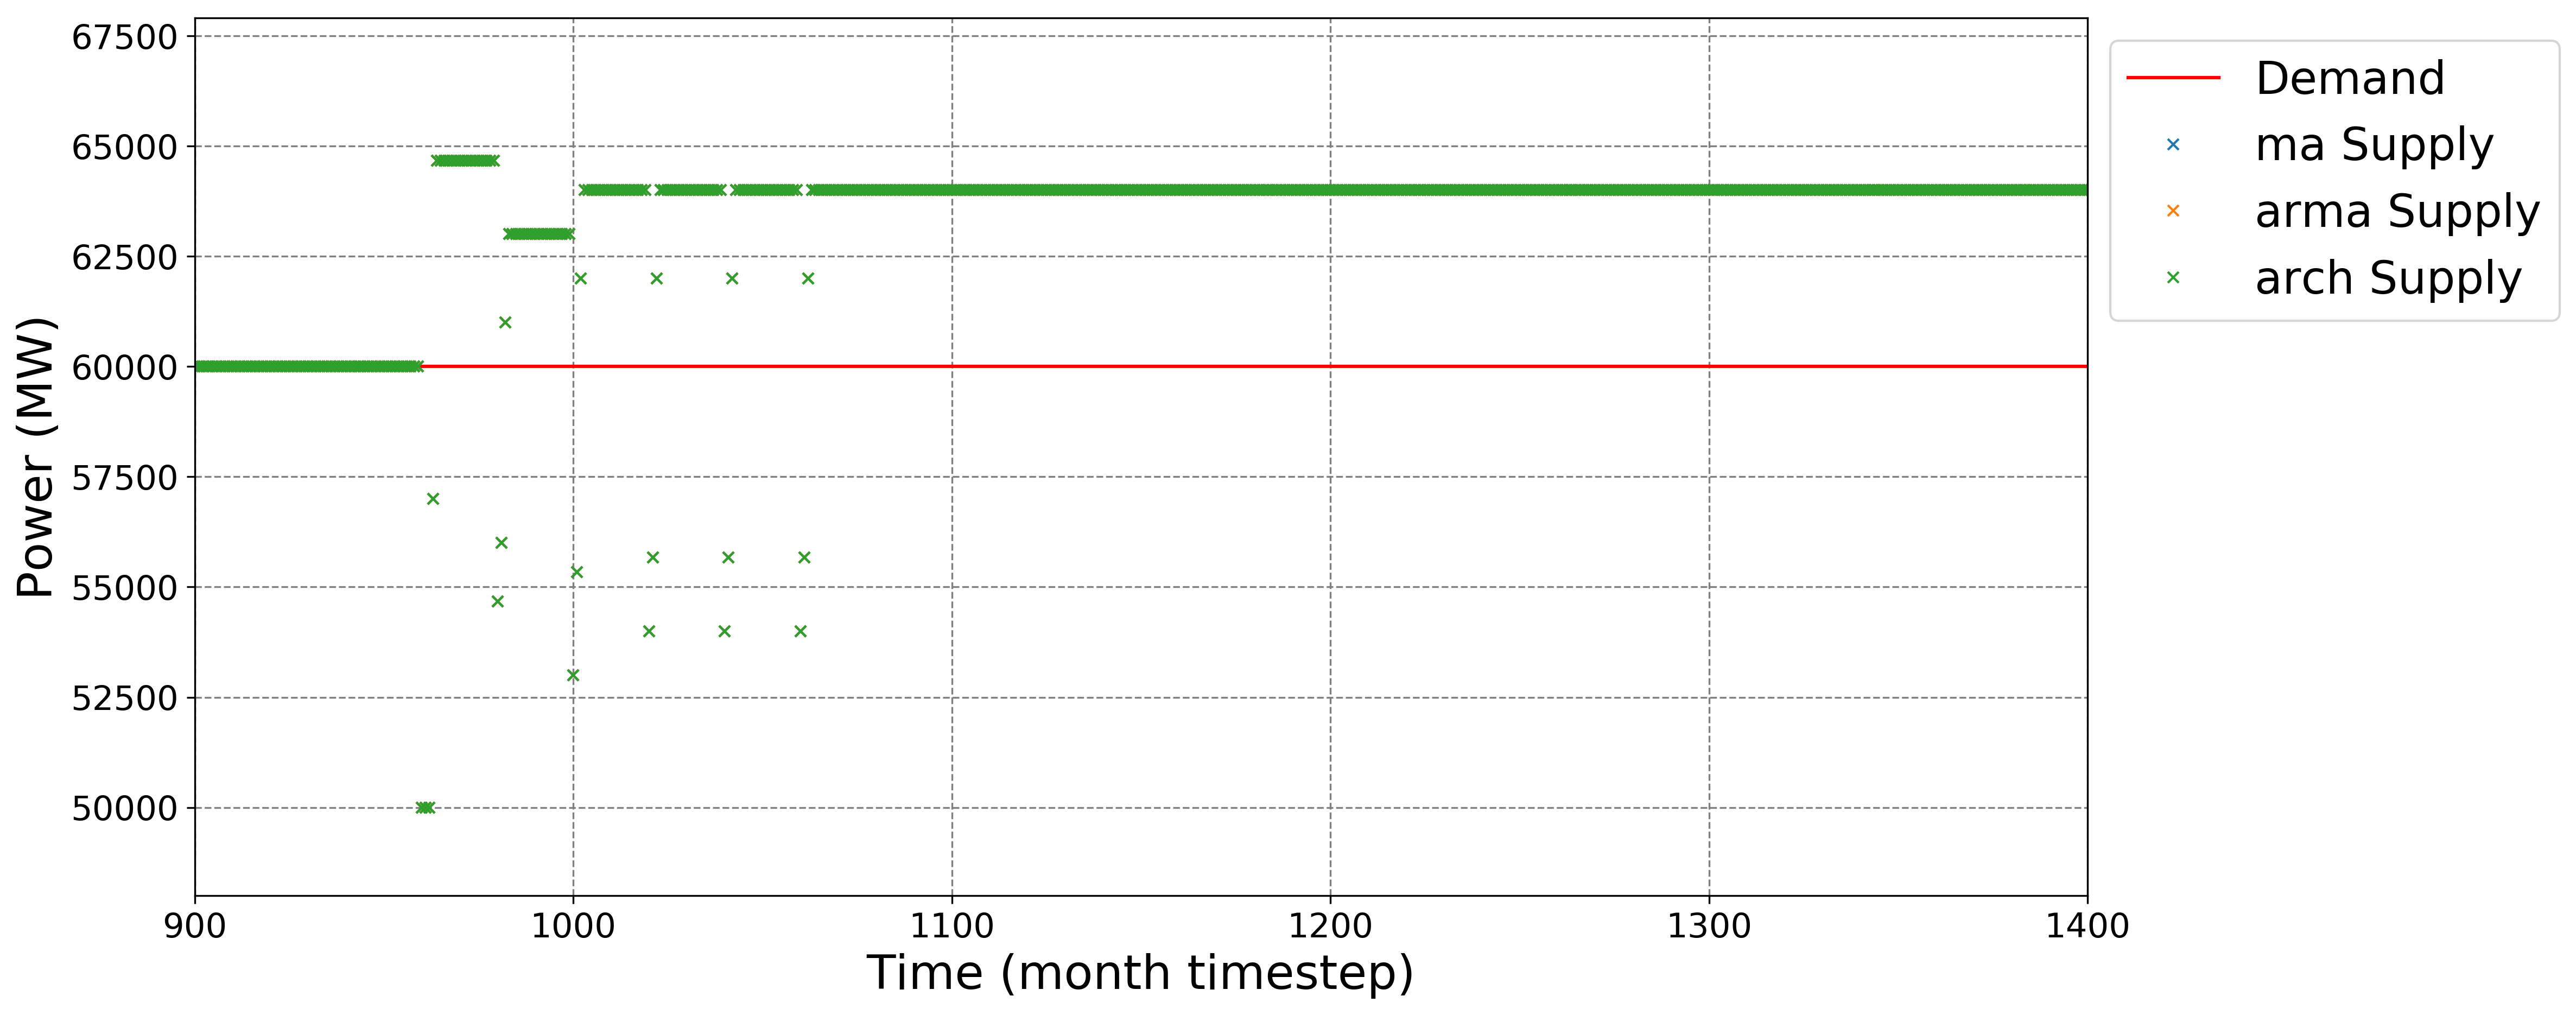
\includegraphics[width=\textwidth]{29-figures/29-power0-buffer01.png} 
	\hfill
	\caption{Constant power demand of 60GW and power supply obtained with the NO algorithms.}
	\label{fig:29-NO}
\end{figure}

\begin{figure}[H]
	\centering
	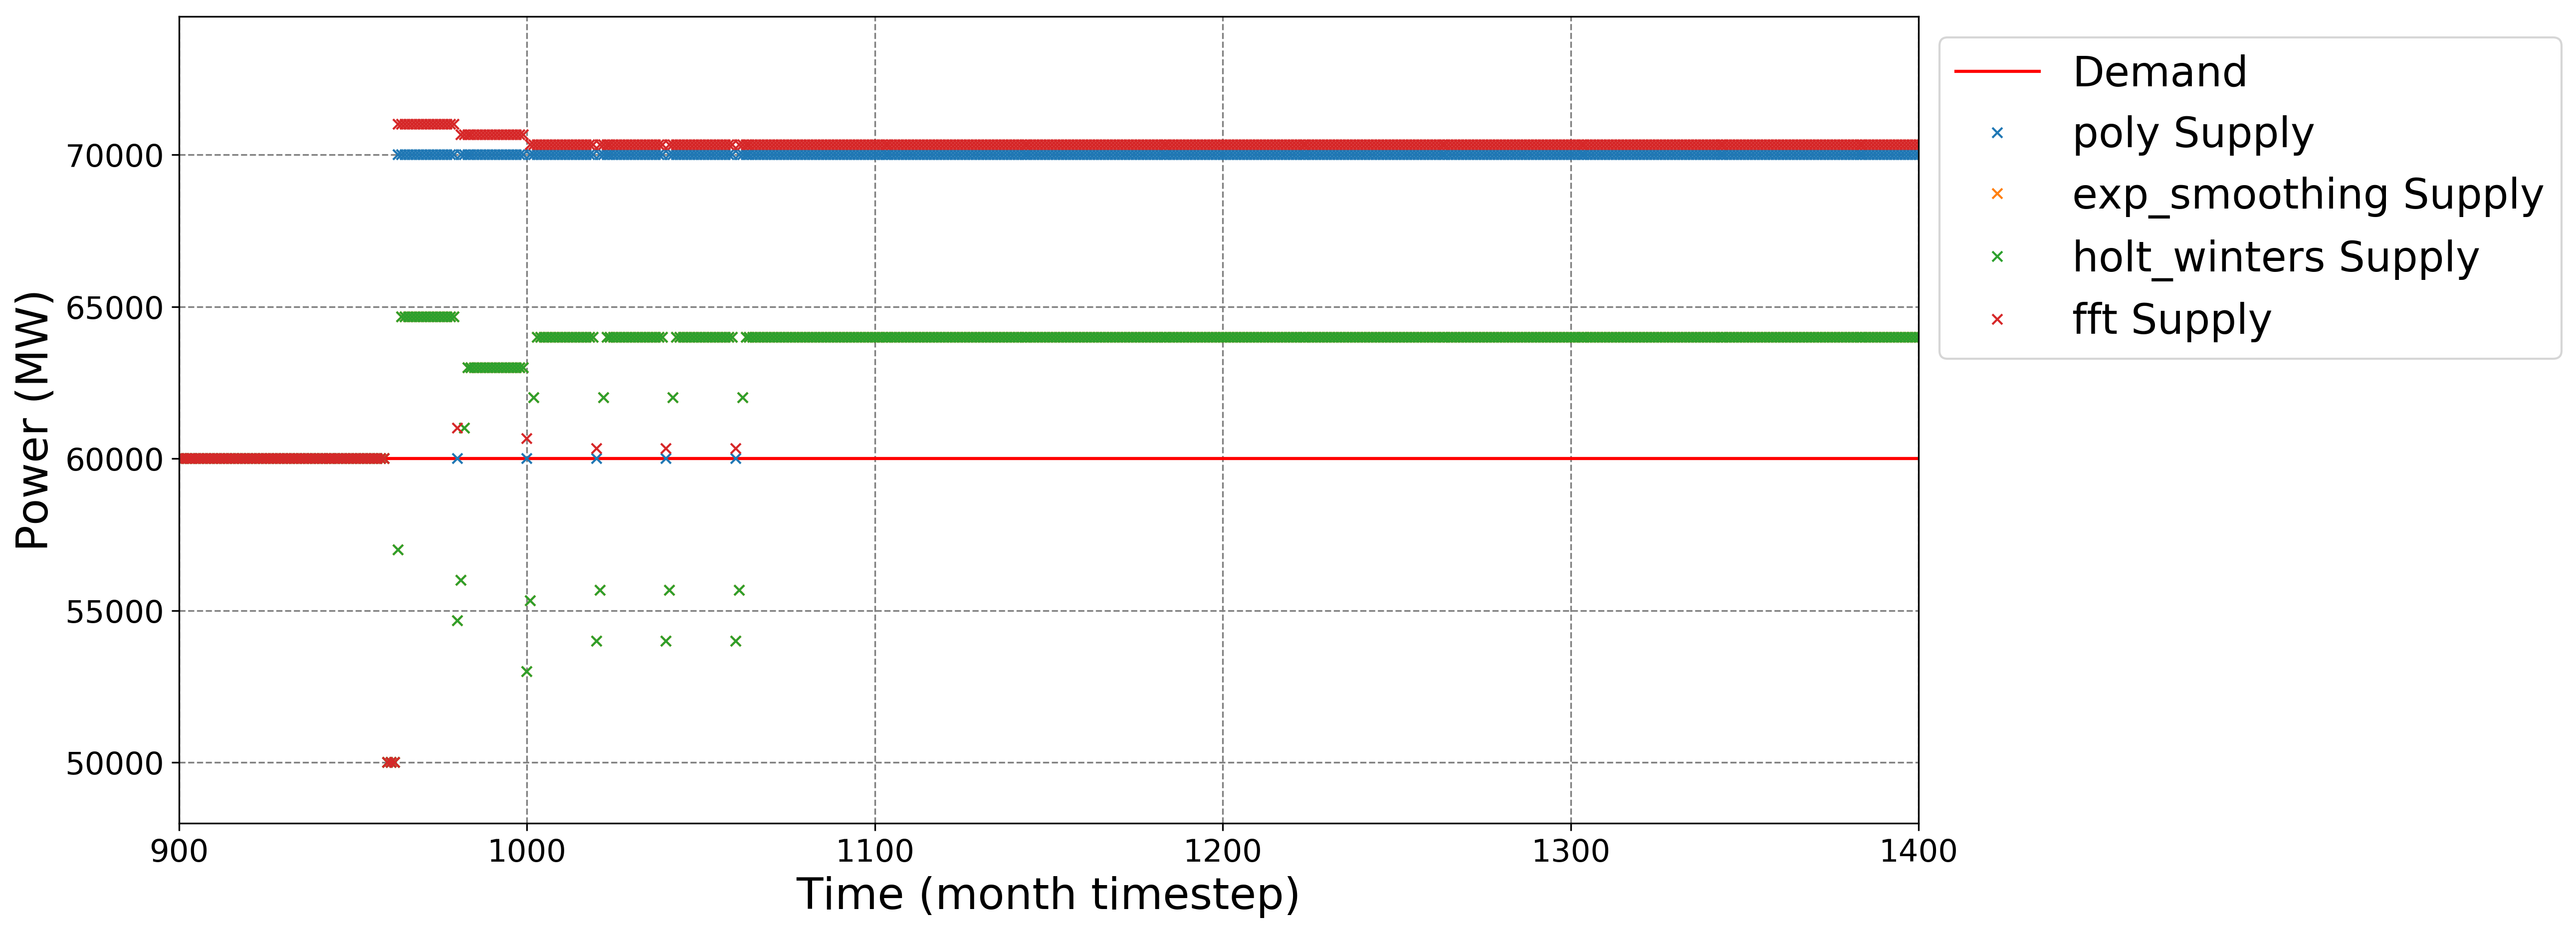
\includegraphics[width=\textwidth]{29-figures/29-power0-buffer02.png} 
	\hfill
	\caption{Constant power demand of 60GW and power supply obtained with the DO algorithms.}
	\label{fig:29-DO}
\end{figure}

\begin{figure}[H]
	\centering
	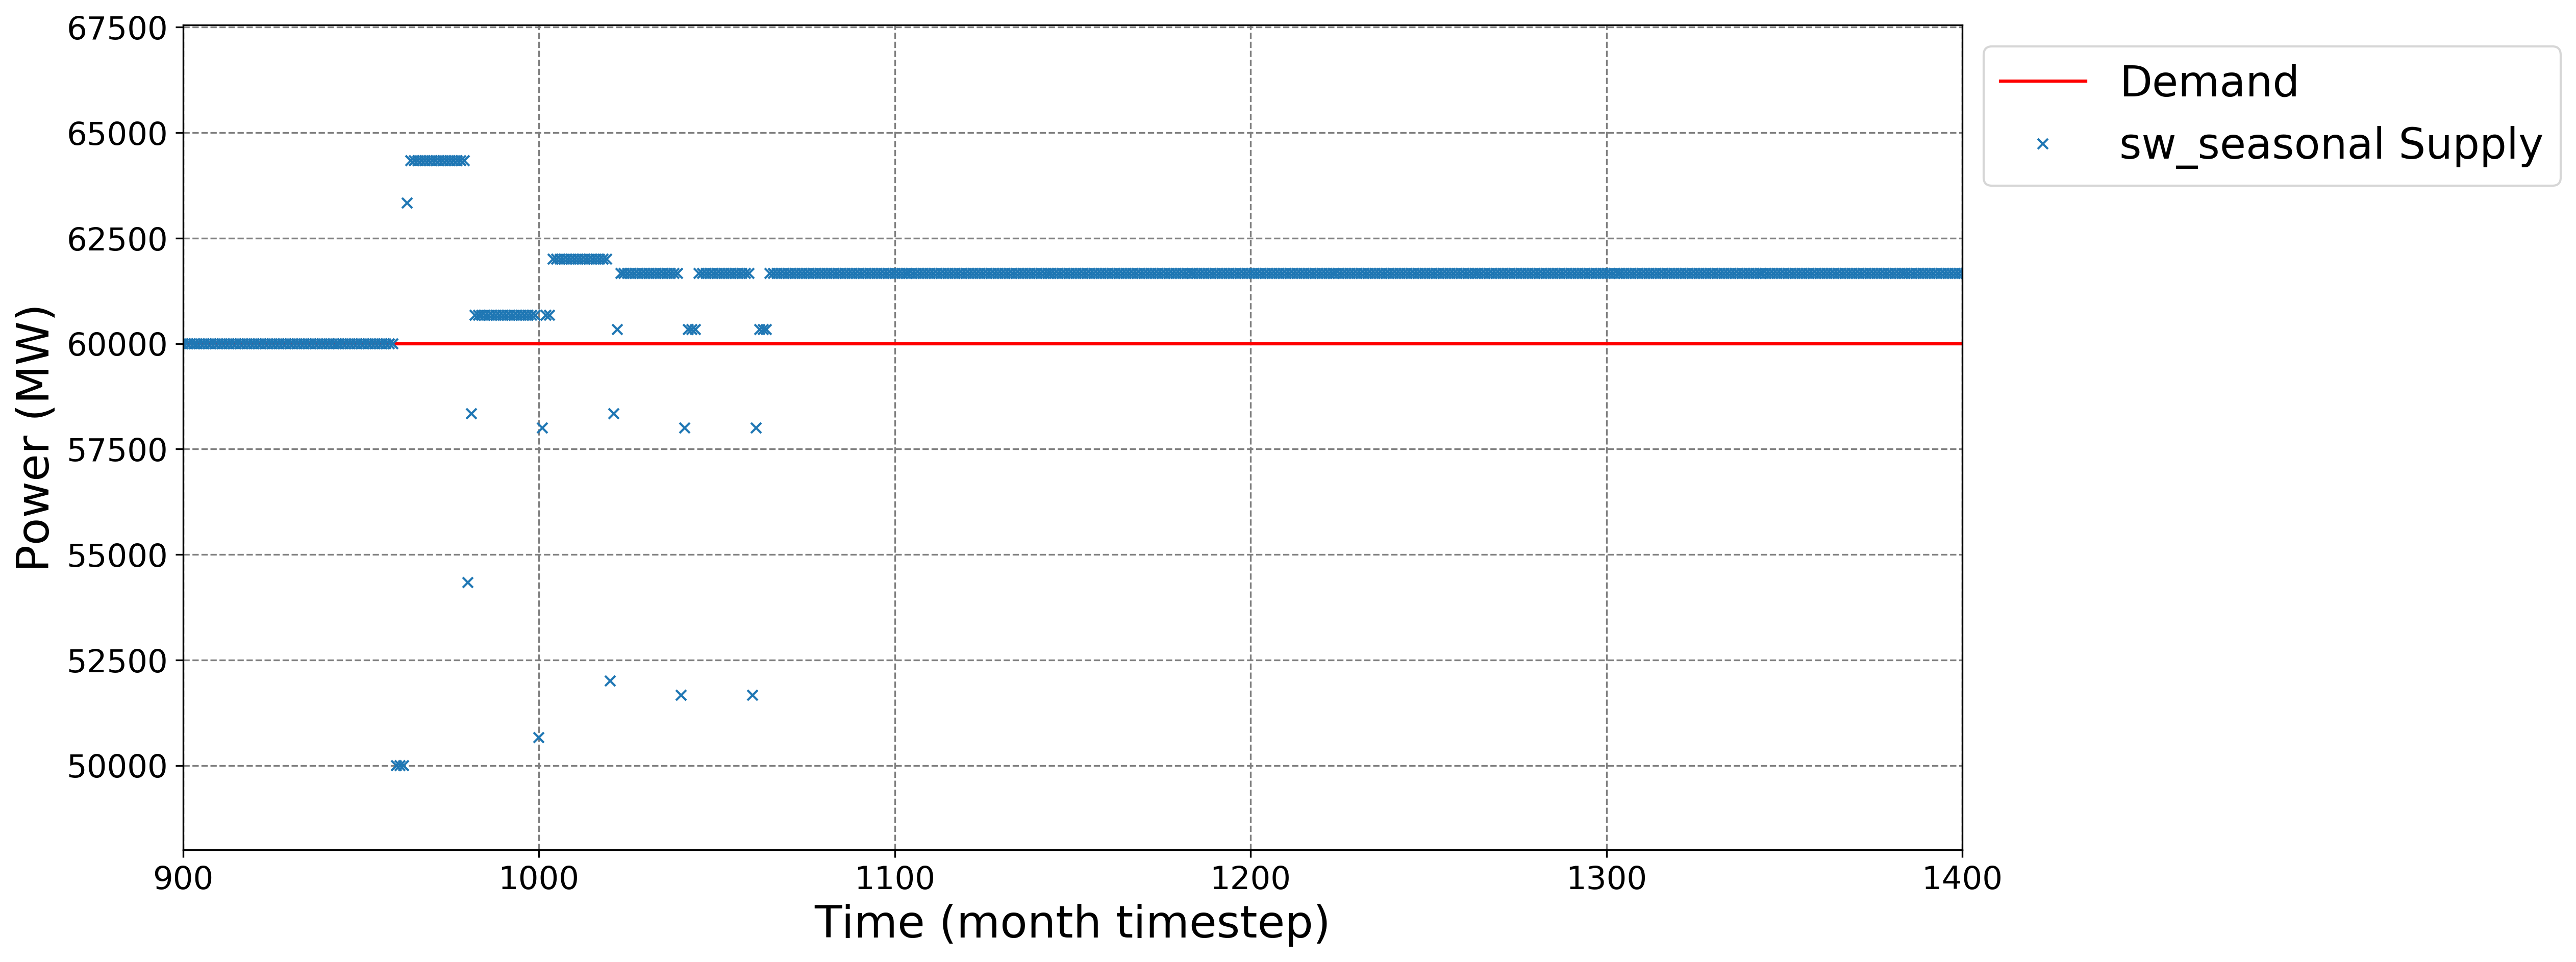
\includegraphics[width=\textwidth]{29-figures/29-power0-buffer03.png} 
	\hfill
	\caption{Constant power demand of 60GW and power supply obtained with the SO algorithms.}
	\label{fig:29-SO}
\end{figure}

\begin{table}[H]
	\centering
	\caption{Undersupply and oversupply of Power for the different prediction 
	method used in EG01-EG29 simulations.}
	\label{tab:29-power}
	\begin{tabularx}{\textwidth}{lRRR}
		\hline
		Algorithm & Undersupplied & Cumulative  & Cumulative \\
		& Timesteps     & Undersupply [GW.mo]  & Oversupply [GW.mo] \\ \hline
		MA        & 15 	& 145.0 & 1847.0 \\ 
		ARMA      & 15 	& 145.0 & 1847.0 \\ 
		ARCH      & 15 	& 145.0 & 1846.9 \\ 
		POLY      &  4 	& 90.0 & 4720.3 \\ 
		EXP\_SMOOTHING 	& 16 & 205.0 & 1847.0 \\ 
		HOLT-WINTERS  	& 16 & 205.0 & 1847.0 \\ 
		FFT       &  5	& 150.0	& 4898.0 \\ 
		SW\_SEASONAL    & 14 & 139.0 & 798.9 \\ \hline
	\end{tabularx}
\end{table}

\subsection{Flat Power Demand: Meaningful commodities}

Using the best prediction method, poly, 
this section presents plots for the supply and demand of the most meaningful 
commodities in the transition scenario.
Table \ref{tab:29-commodities} summarizes which commodity each figure in
this section corresponds to. 
Table \ref{tab:29-commod} presents the number of steps of undersupply, 
cumulative undersupply, and cumulative oversupply of such commodities.

\begin{table}[H]
	\centering
	\caption{Table of figures of commodities in the simulation of EG01-EG29.}
	\label{tab:29-commodities}
	\begin{tabularx}{\textwidth}{lL}
		\hline
		Commodity & Figure \\ \hline
		Power           & \ref{fig:29-power} \\
		Natural-U       & \ref{fig:29-sourceout} \\
		Enriched-U   	& \ref{fig:29-enrichmentout} \\
		FR fuel       	& \ref{fig:29-frmixerout} \\
		MOX LWR fuel   	& \ref{fig:29-moxmixerout} \\
		Reprocessed Pu from spent fuel of LWRs & \ref{fig:29-pu1} \\
		Reprocessed Pu from spent fuel of FRs  & \ref{fig:29-frpu} \\
		Reprocessed Pu from spent fuel of MOX LWRs  & \ref{fig:29-moxpu} \\ \hline
	\end{tabularx}
\end{table}

\begin{figure}[H]
	\centering
	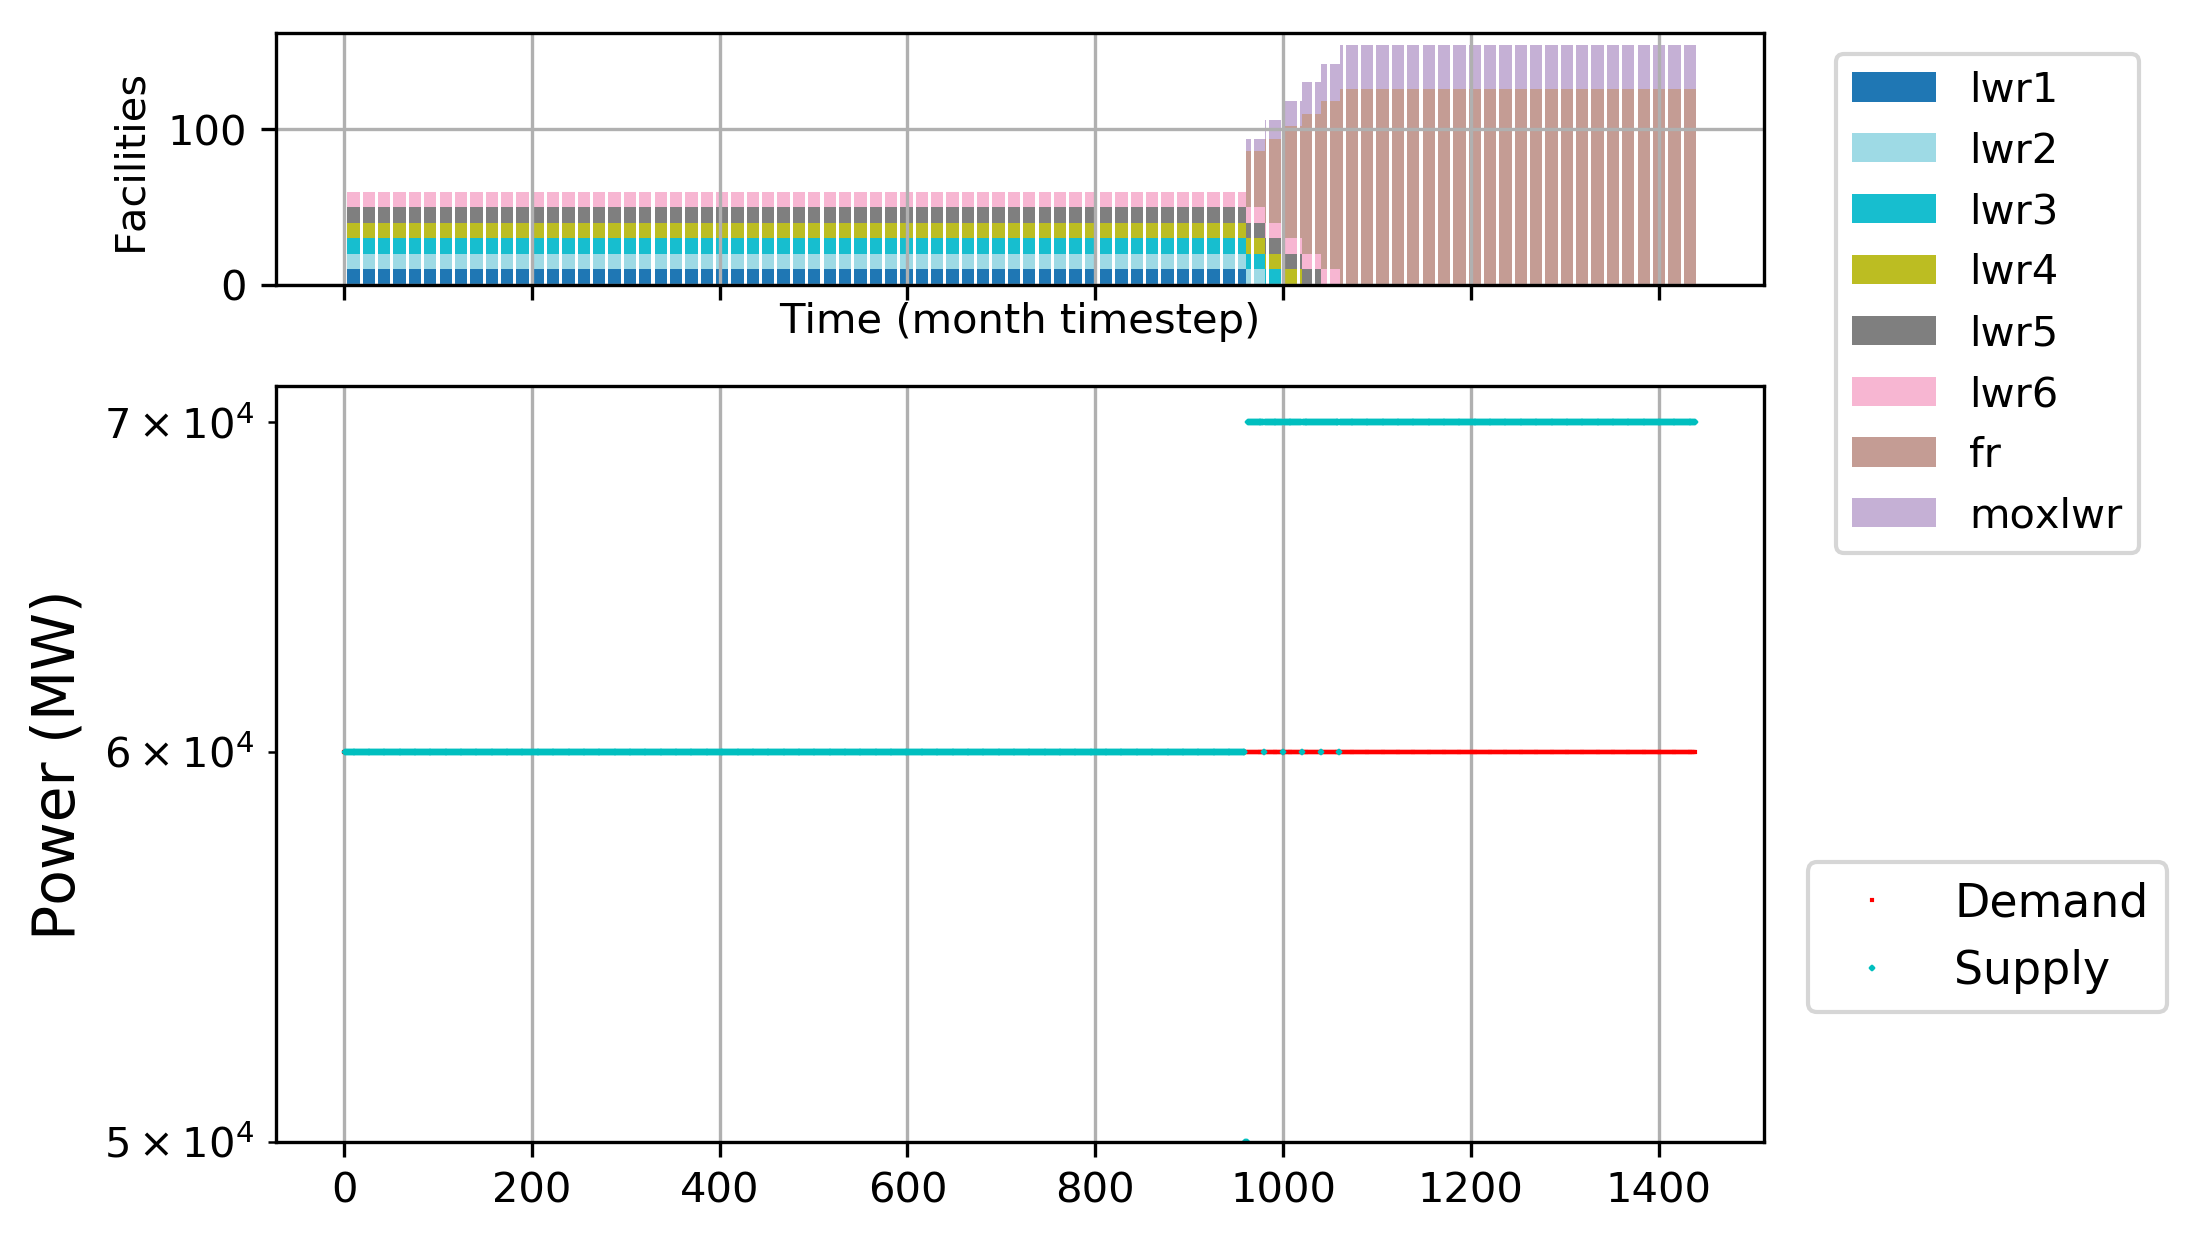
\includegraphics[width=\textwidth]{29-figures/0-poly-power.png} 
	\hfill
	\caption{Demand and supply of Power and number of reactors deployed.}
	\label{fig:29-power}
\end{figure}

\begin{figure}[H]
	\centering
	\begin{subfigure}[]{0.45\textwidth}
		\centering
		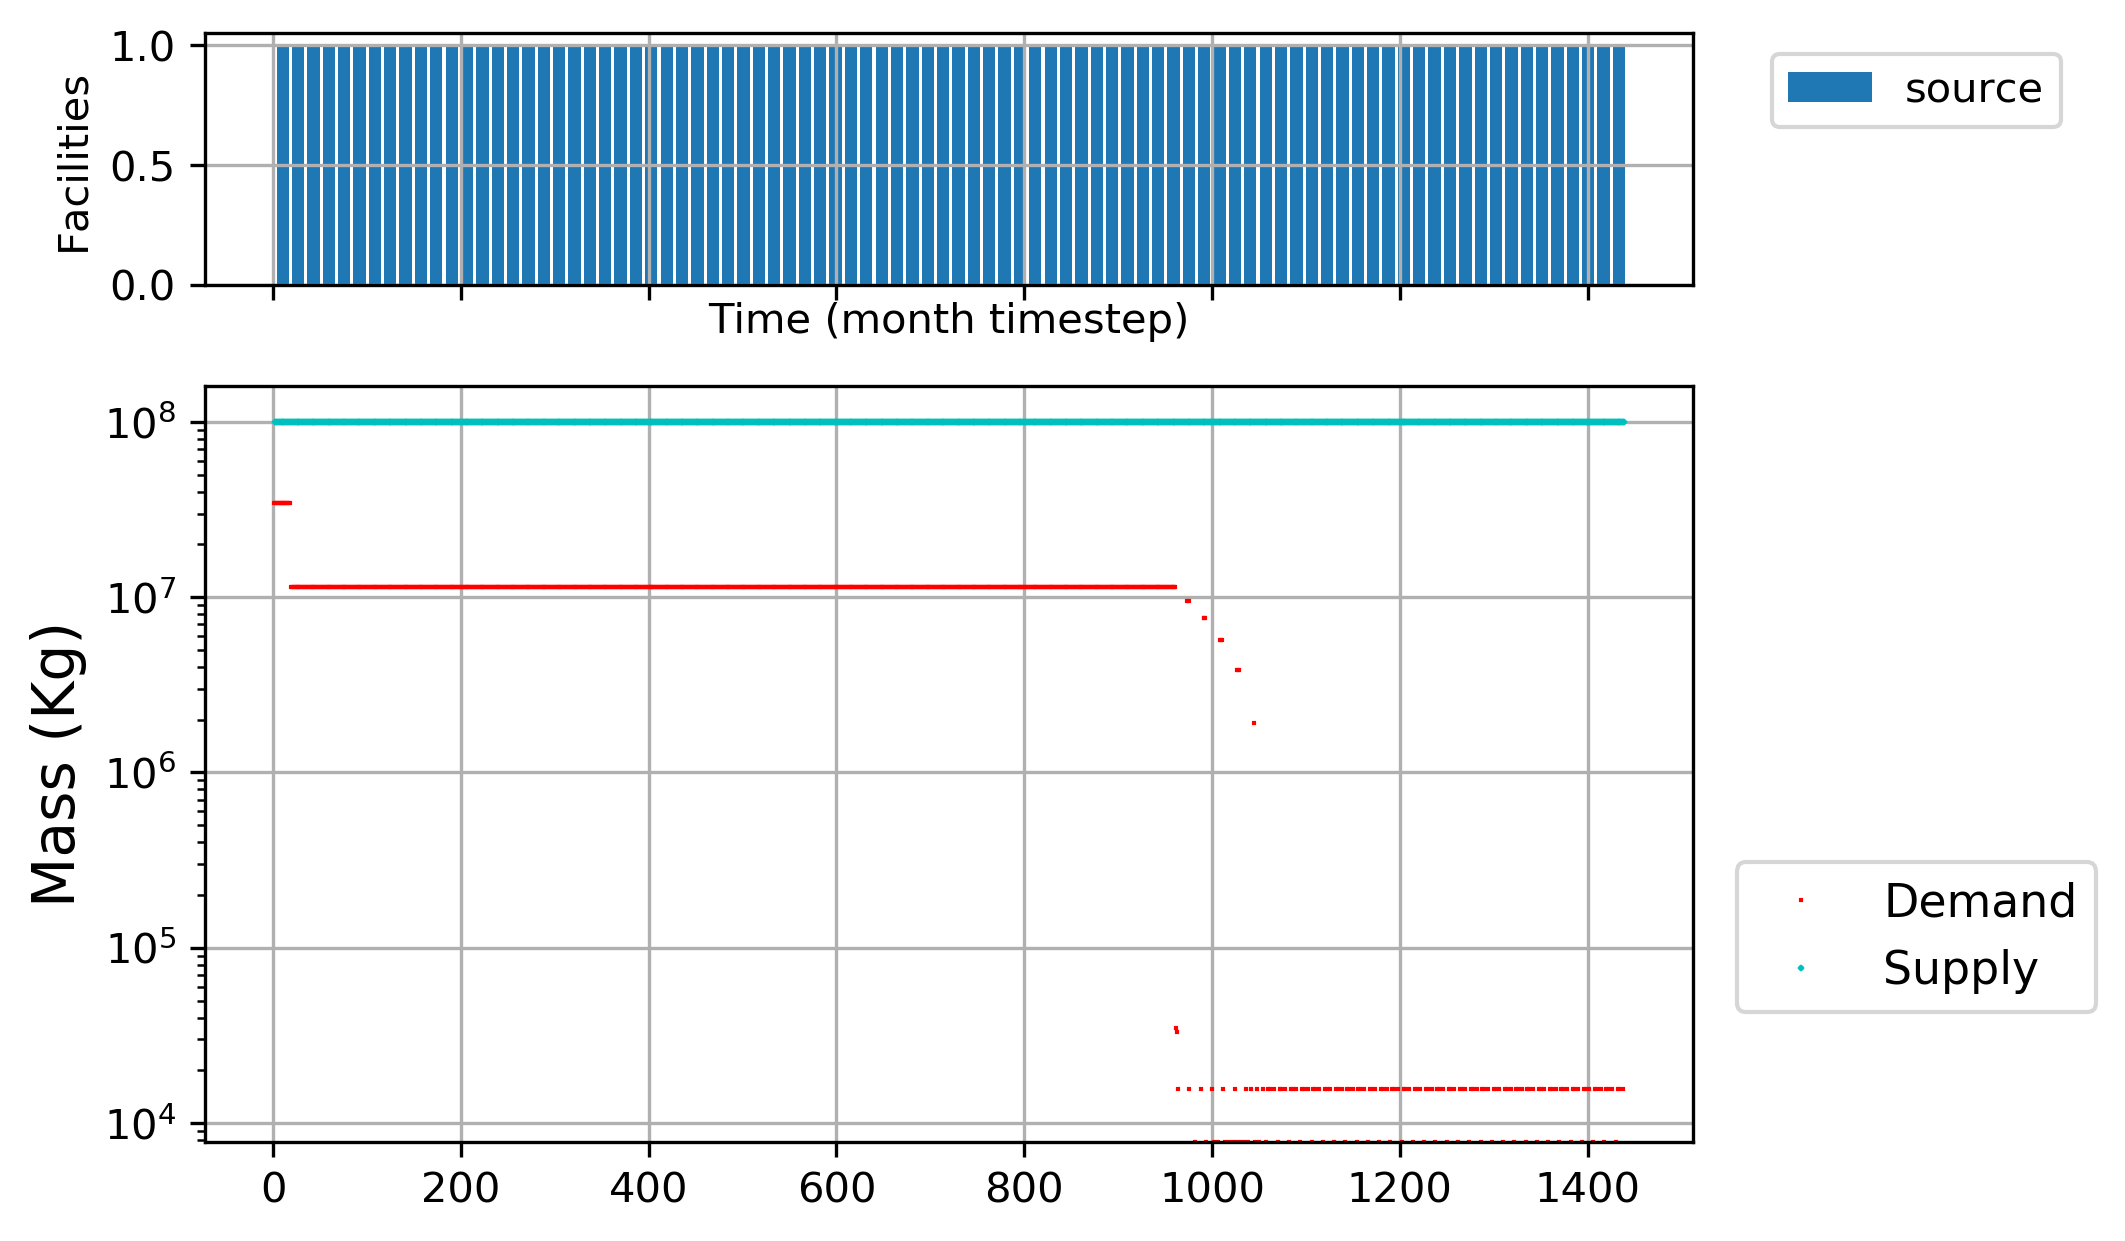
\includegraphics[width=\linewidth]{29-figures/0-poly-sourceout.png} 
		\caption{Natural-U.}
		\label{fig:29-sourceout}
	\end{subfigure}
	\vspace{1cm}
	\begin{subfigure}[]{0.45\textwidth}
		\centering
		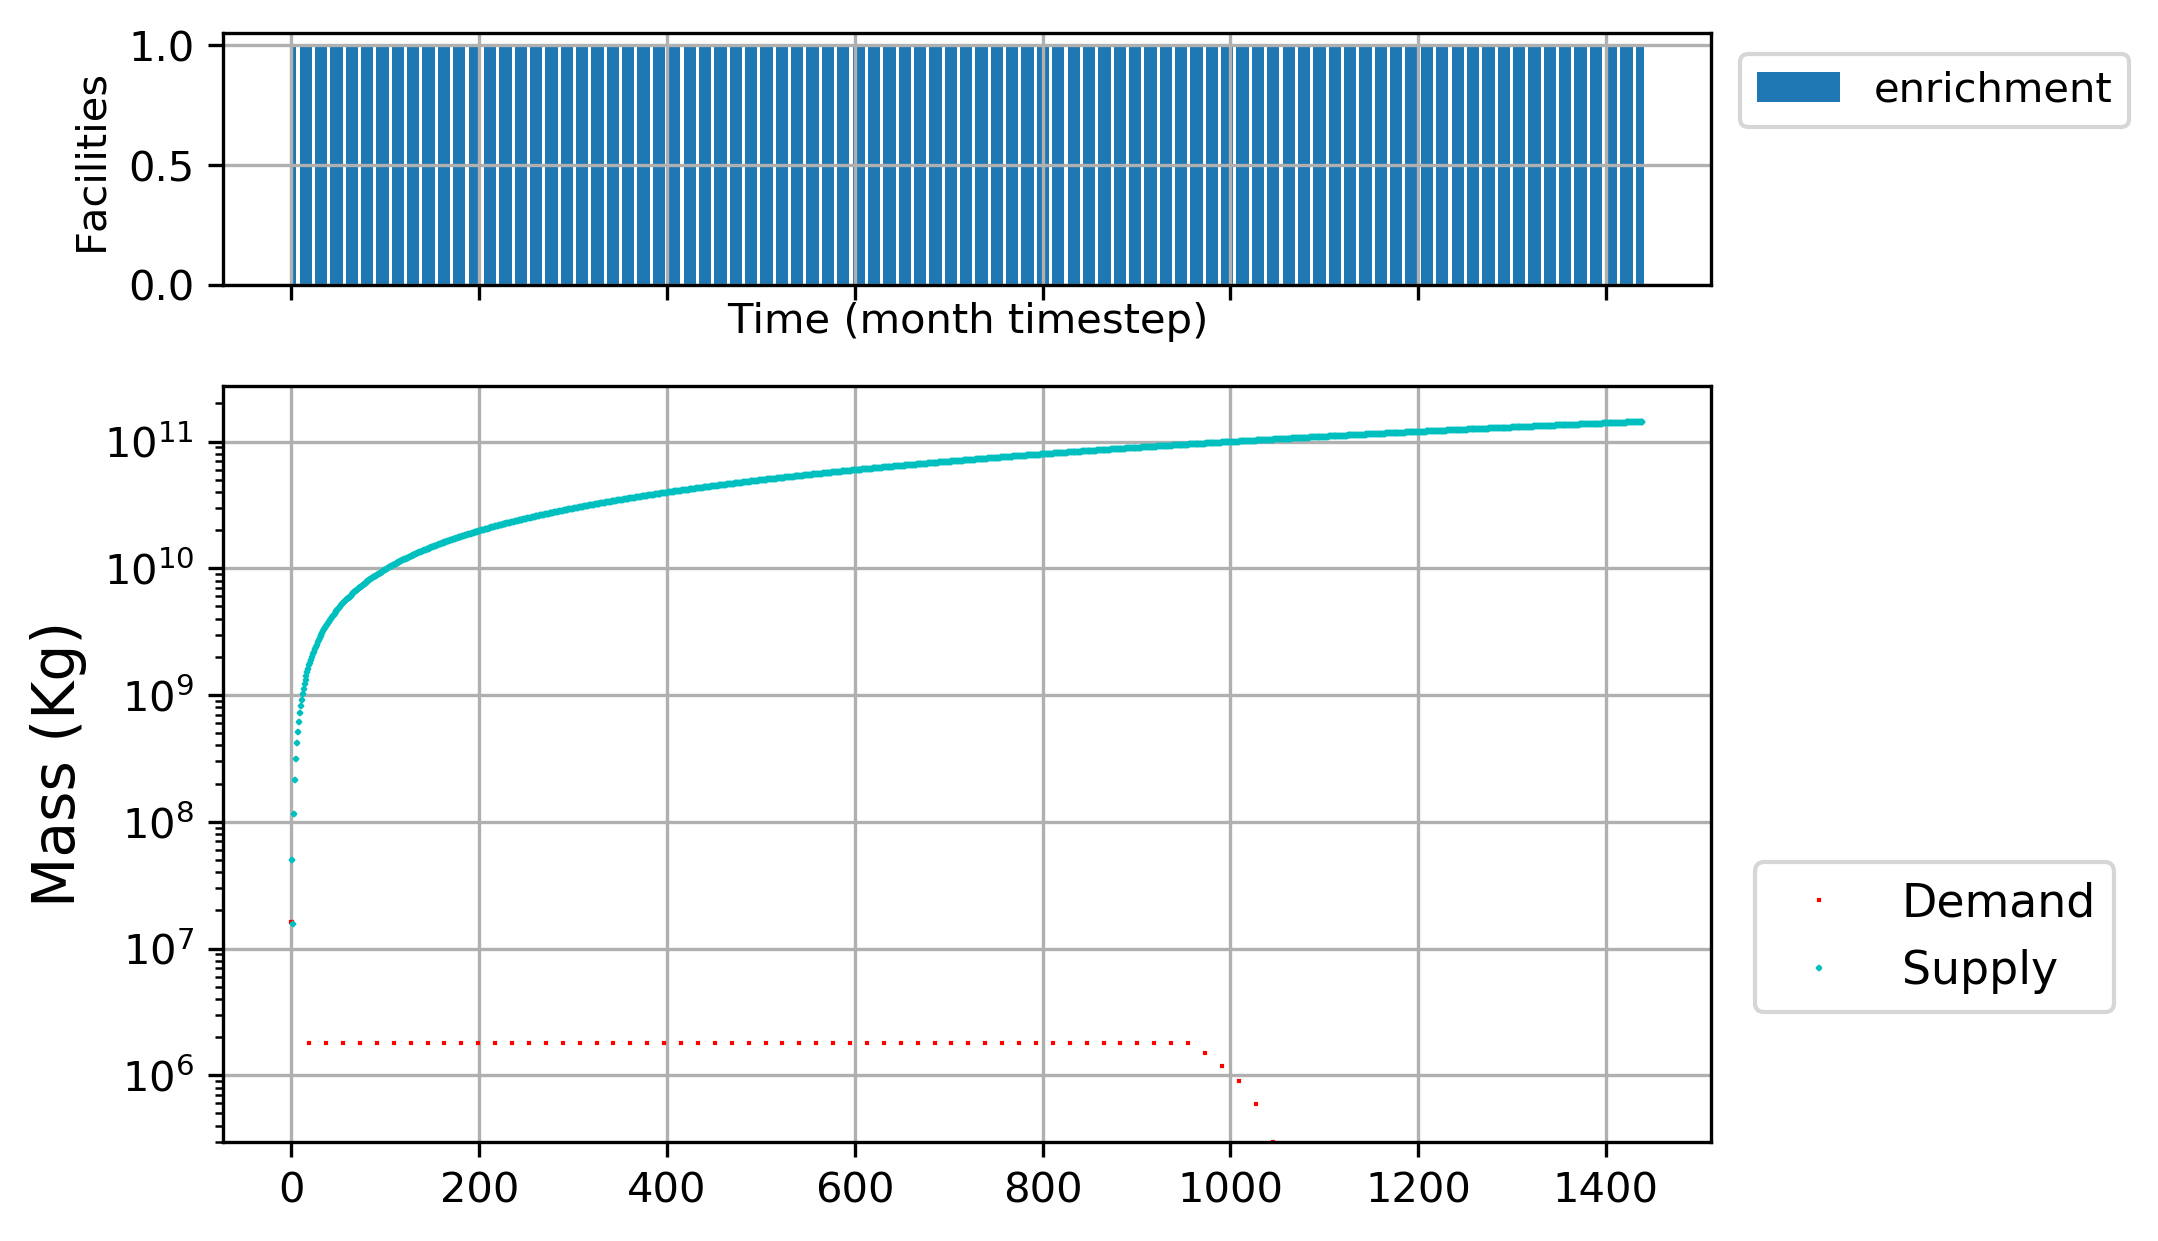
\includegraphics[width=\linewidth]{29-figures/0-poly-enrichmentout.png} 
		\caption{Enriched-U.}
		\label{fig:29-enrichmentout}
	\end{subfigure}
	\hfill
	\caption{Demand and supply of different commodities and number of facilities that produce them.}
	\label{fig:29-front}
\end{figure}

\begin{figure}[H]
	\centering
	\begin{subfigure}[]{0.45\textwidth}
		\centering
		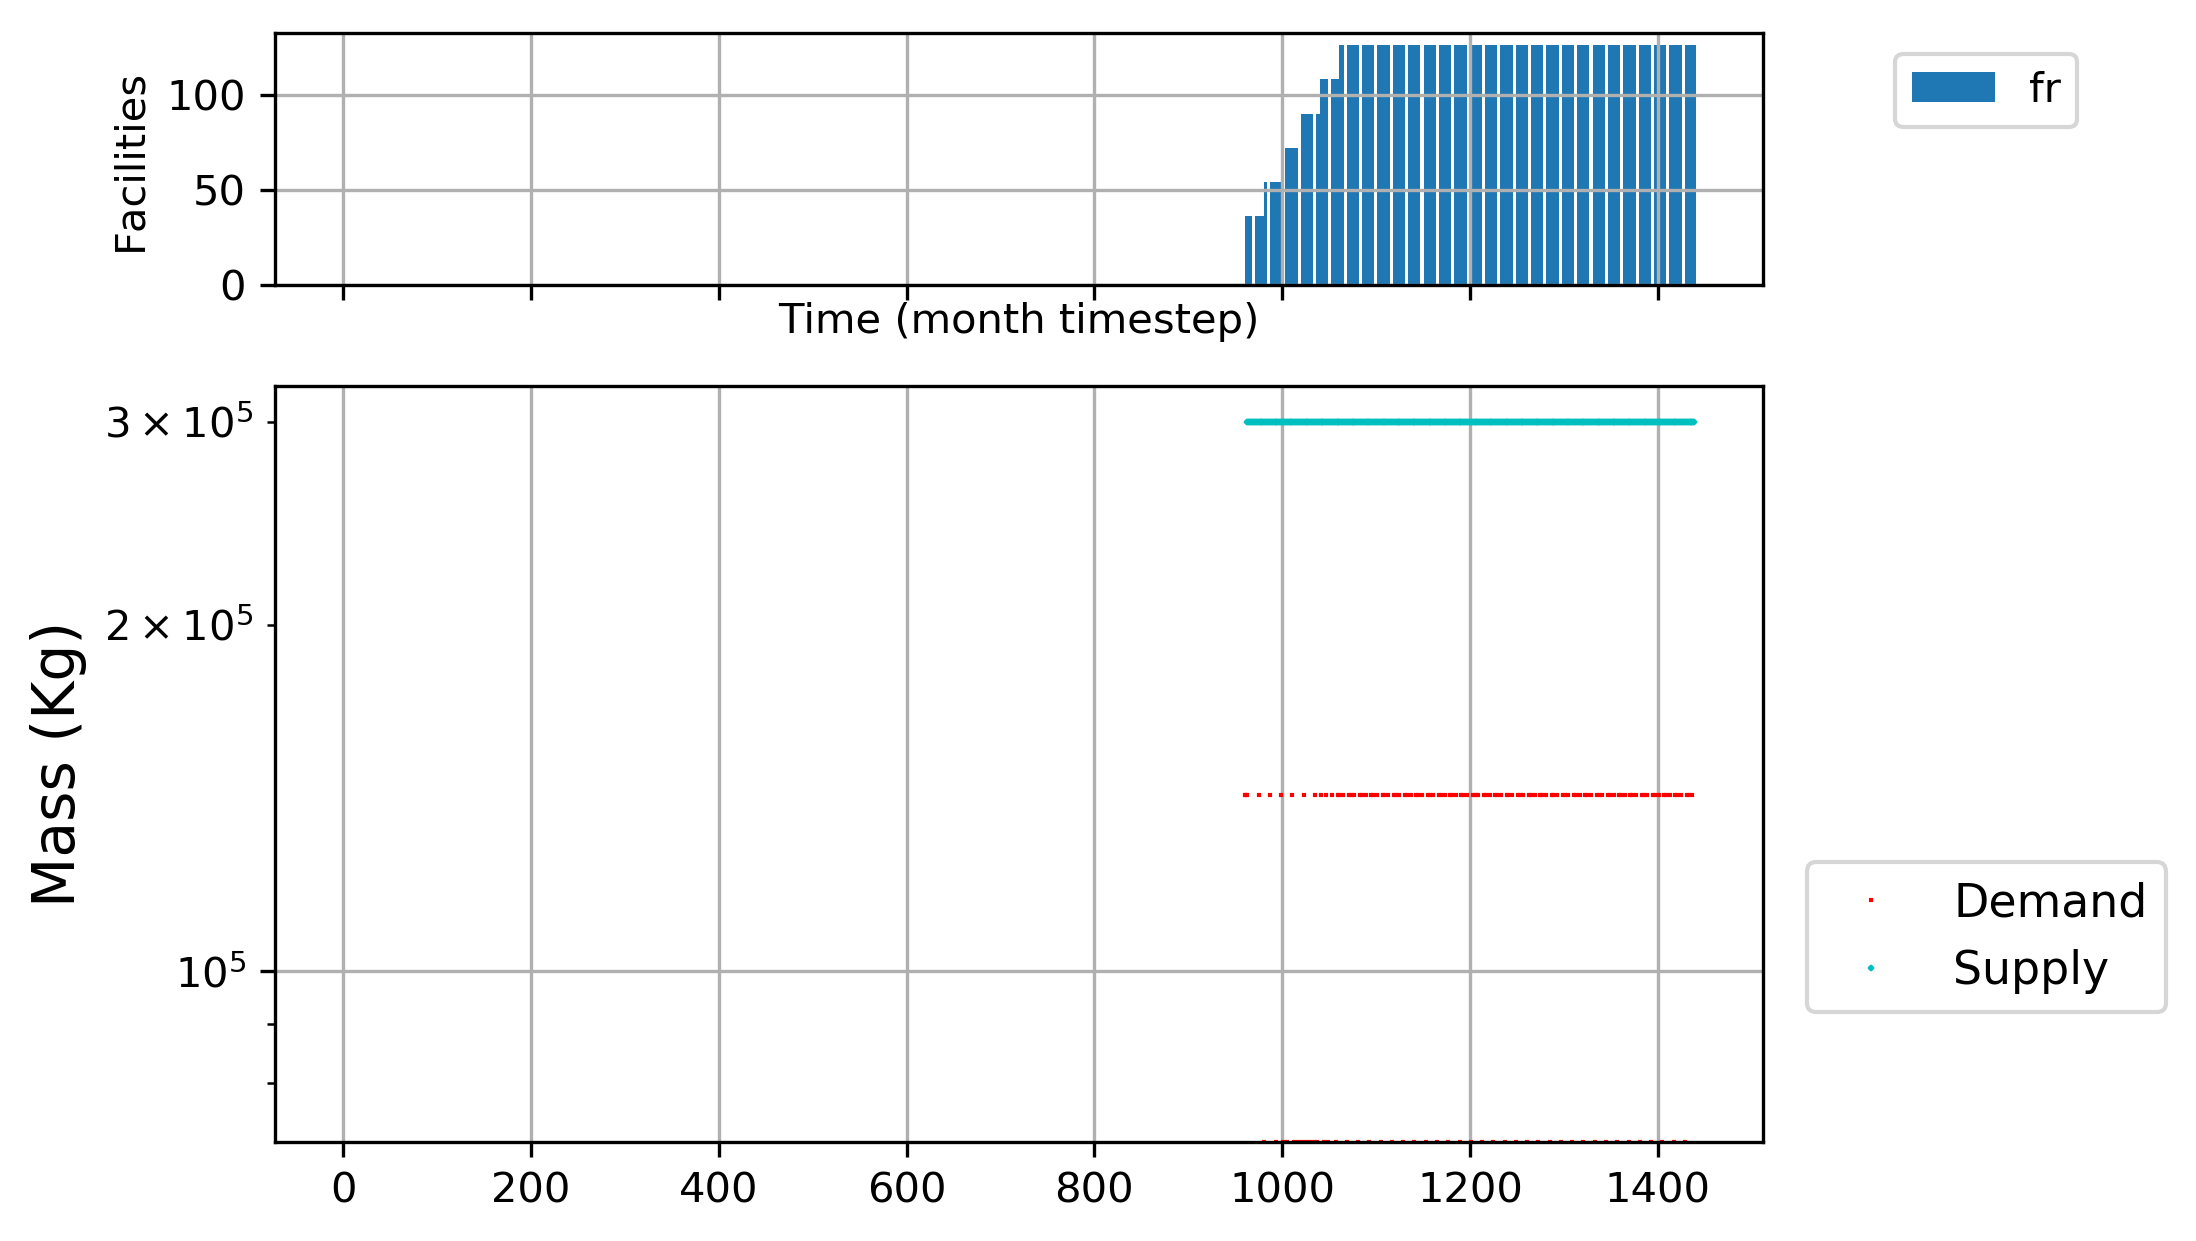
\includegraphics[width=\linewidth]{29-figures/0-poly-frmixerout.png} 
		\caption{FR Fuel.}
		\label{fig:29-frmixerout}
	\end{subfigure}
	\vspace{1cm}
	\begin{subfigure}[]{0.45\textwidth}
		\centering
		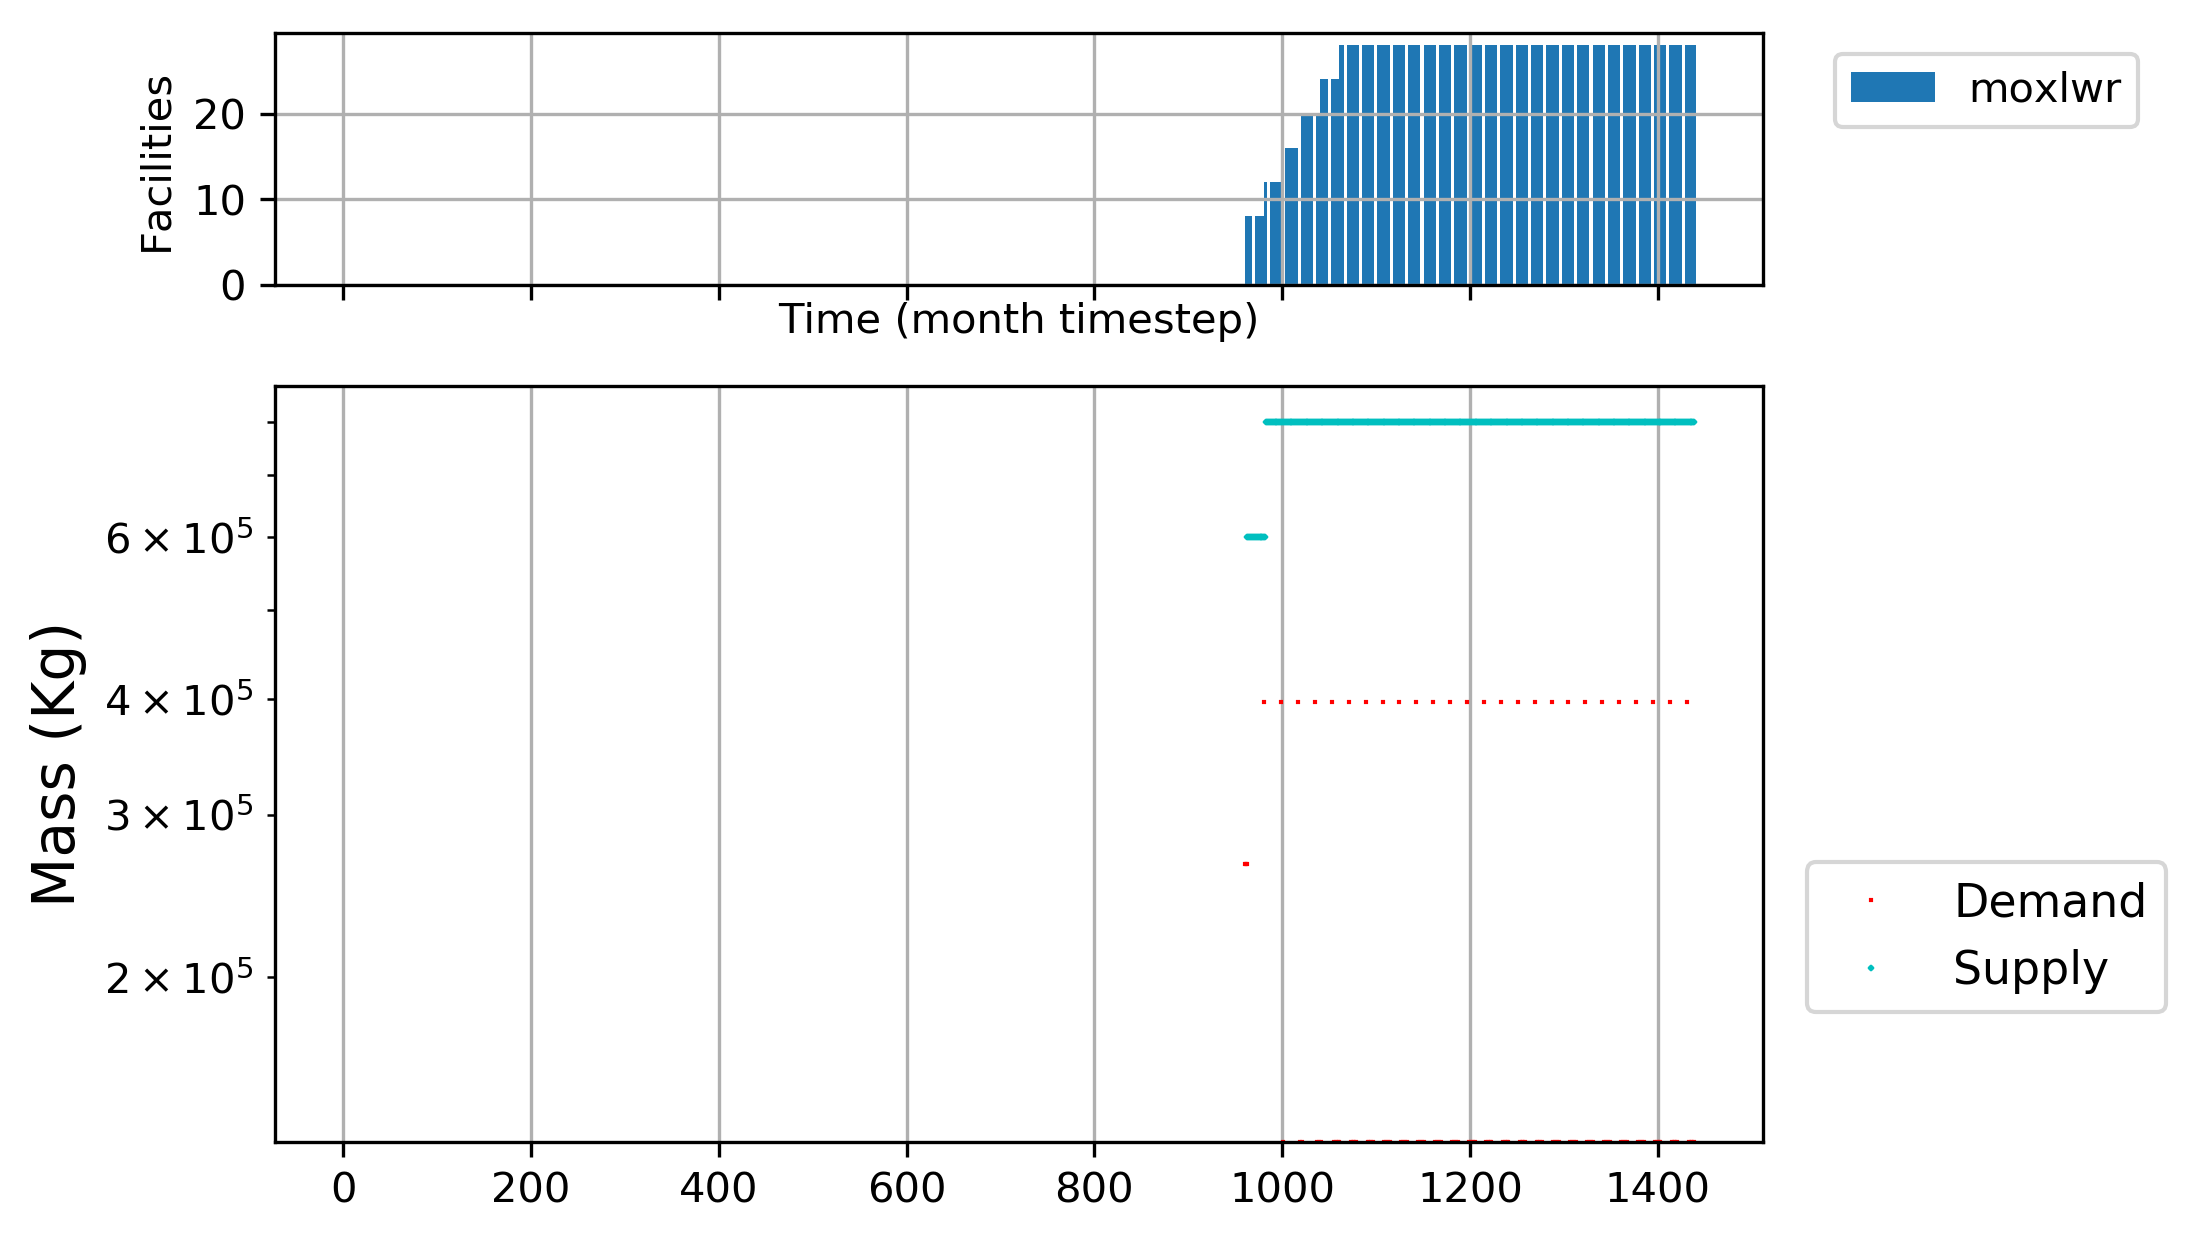
\includegraphics[width=\linewidth]{29-figures/0-poly-moxmixerout.png} 
		\caption{MOX LWR Fuel.}
		\label{fig:29-moxmixerout}
	\end{subfigure}
	\hfill
	\caption{Demand and supply of fuel and number of reactors.}
	\label{fig:29-mix}
\end{figure}

\begin{figure}[H]
	\centering
	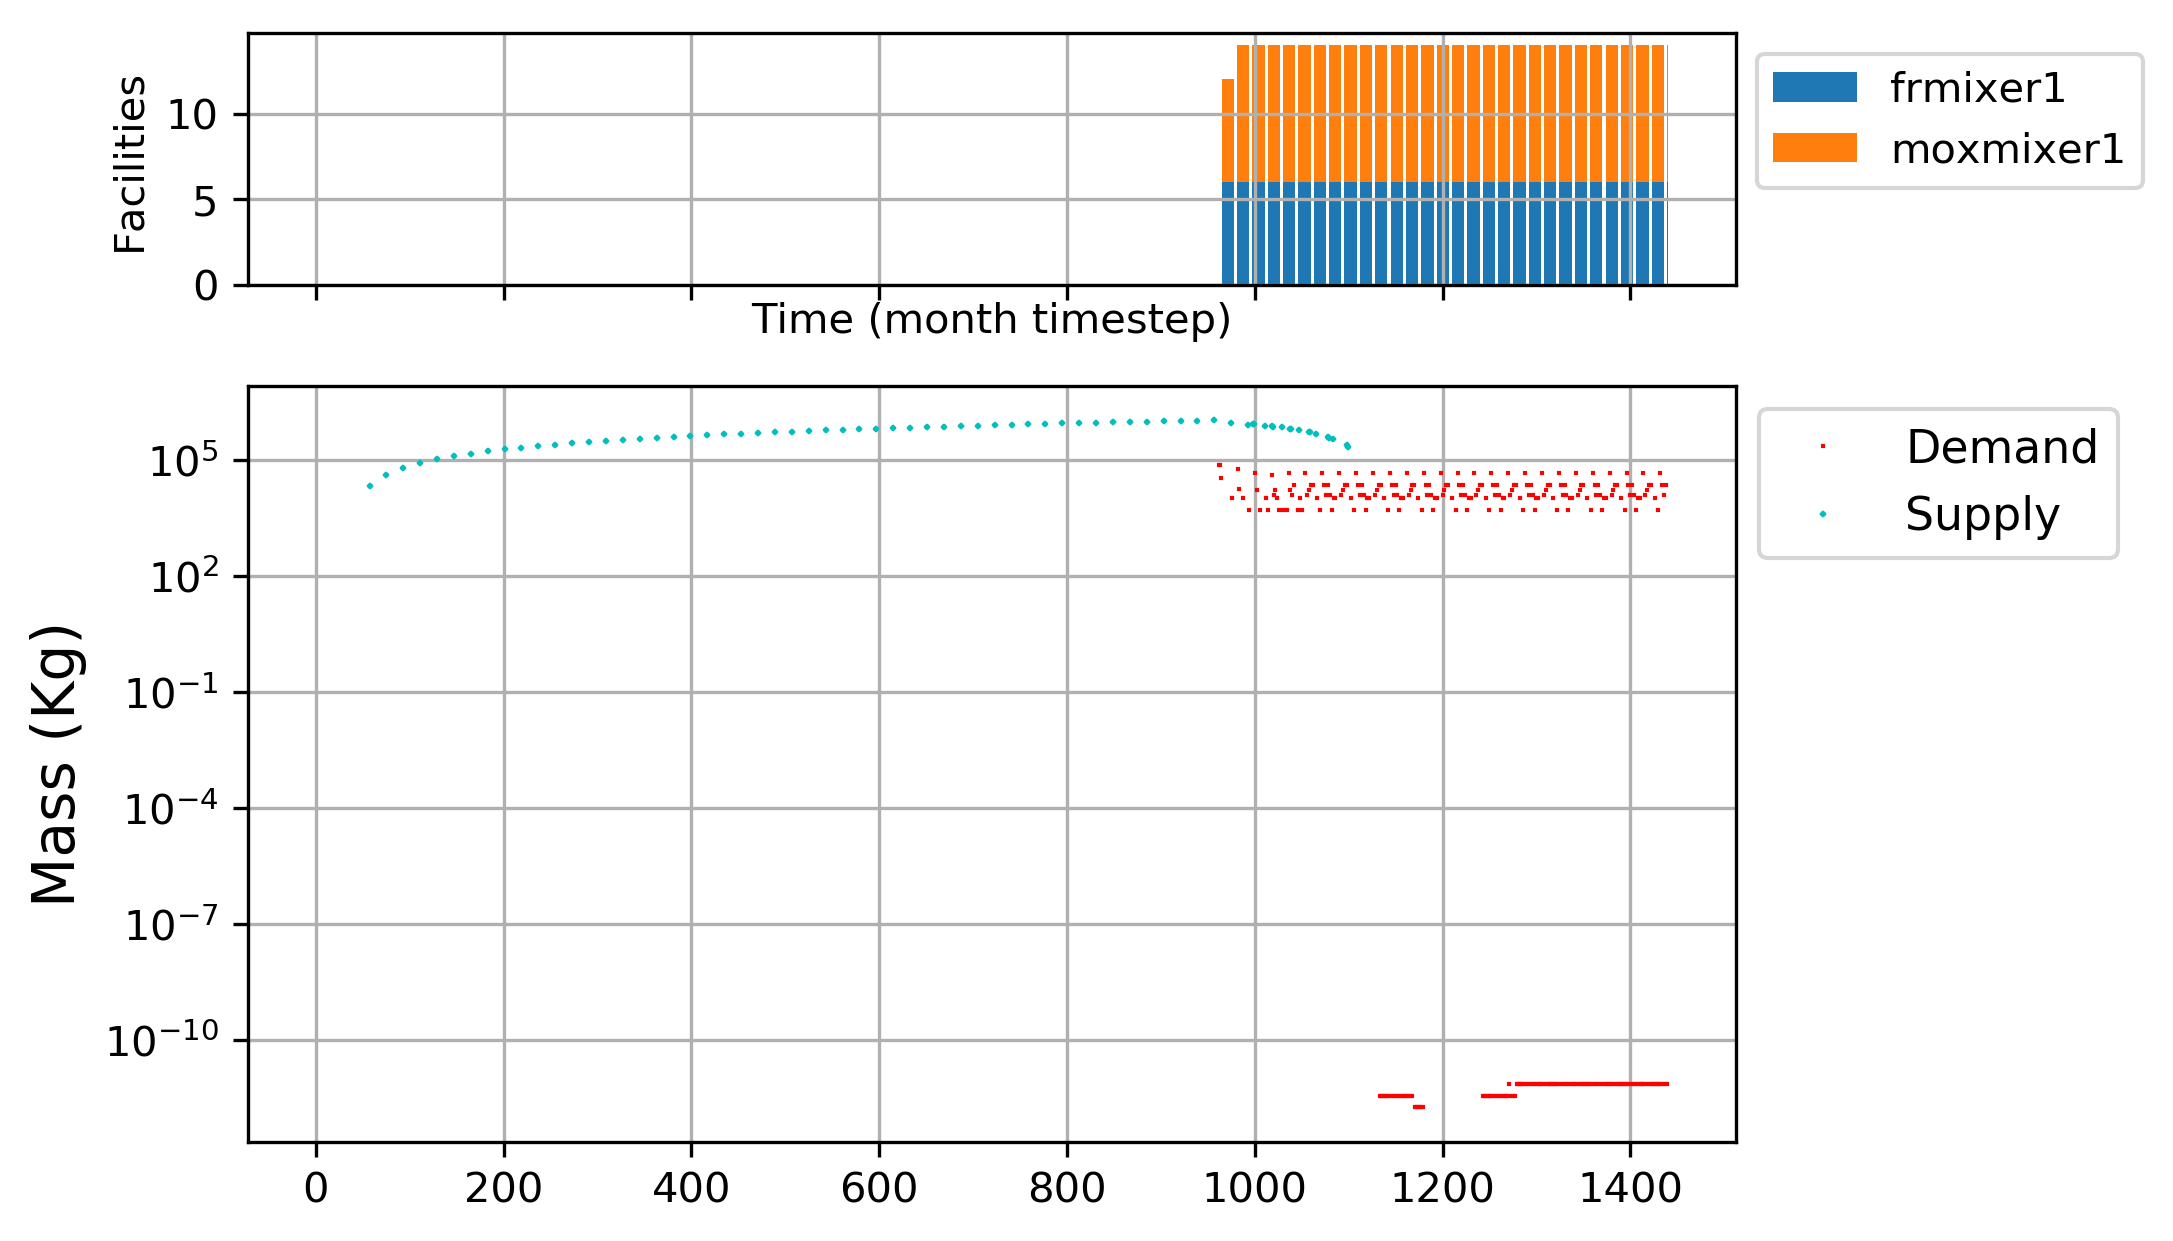
\includegraphics[width=\textwidth]{29-figures/0-poly-lwrpu.png} 
	\hfill
	\caption{Demand and supply of reprocessed Pu from spent fuel of LWRs and number of facilities supplied with them.}
	\label{fig:29-pu1}
\end{figure}

\begin{figure}[H]
	\centering
	\begin{subfigure}[t]{0.45\textwidth}
		\centering
		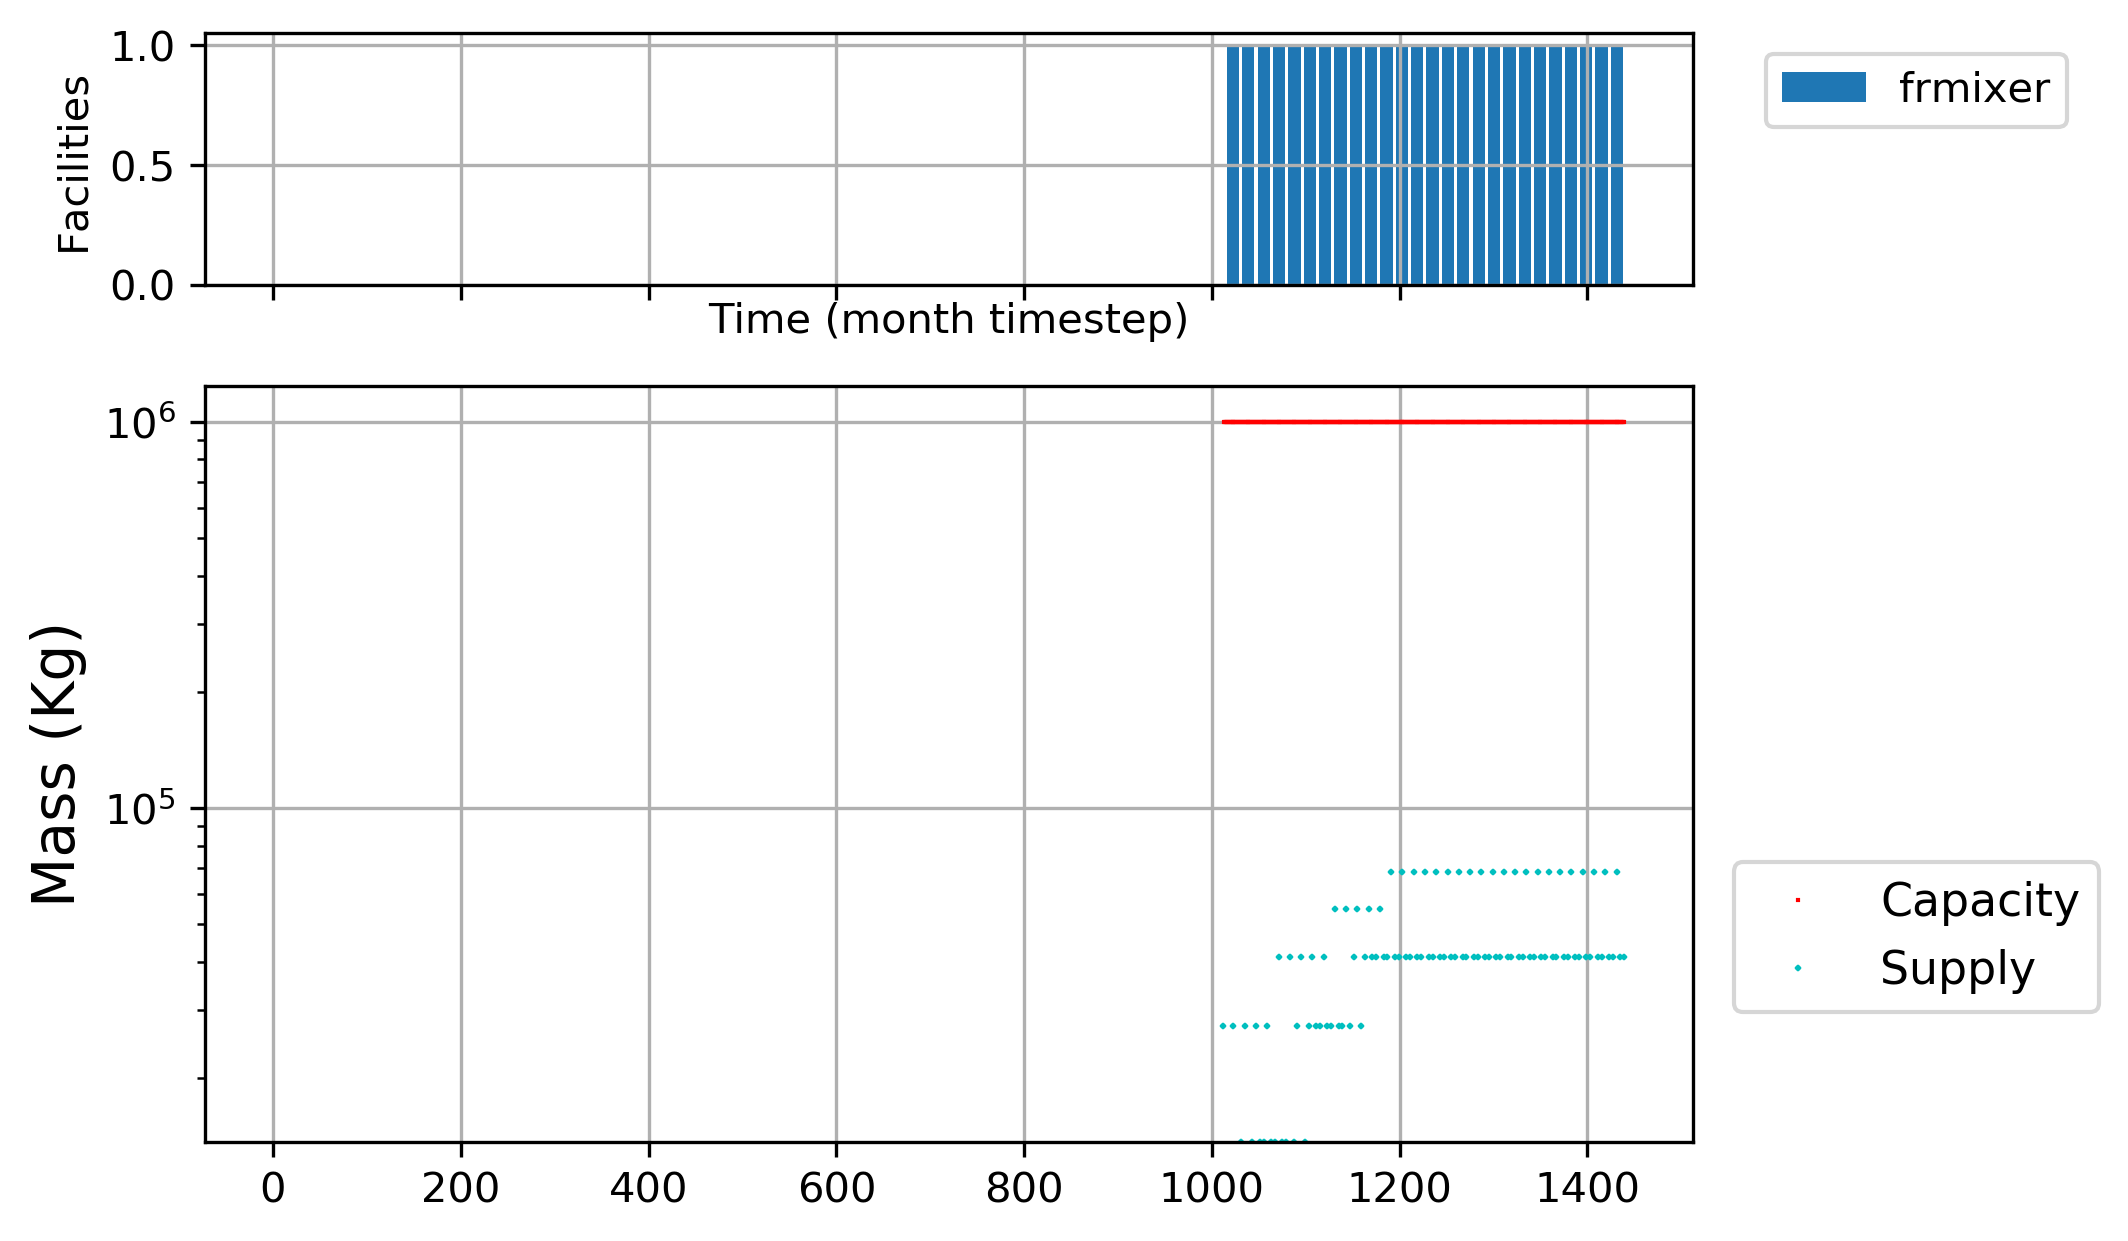
\includegraphics[width=\linewidth]{23-figures/0-poly-frpu.png} 
		\caption{Reprocessed Pu from spent fuel of FRs.}
		\label{fig:29-frpu}
	\end{subfigure}
	\vspace{1cm}
	\begin{subfigure}[t]{0.45\textwidth}
		\centering
		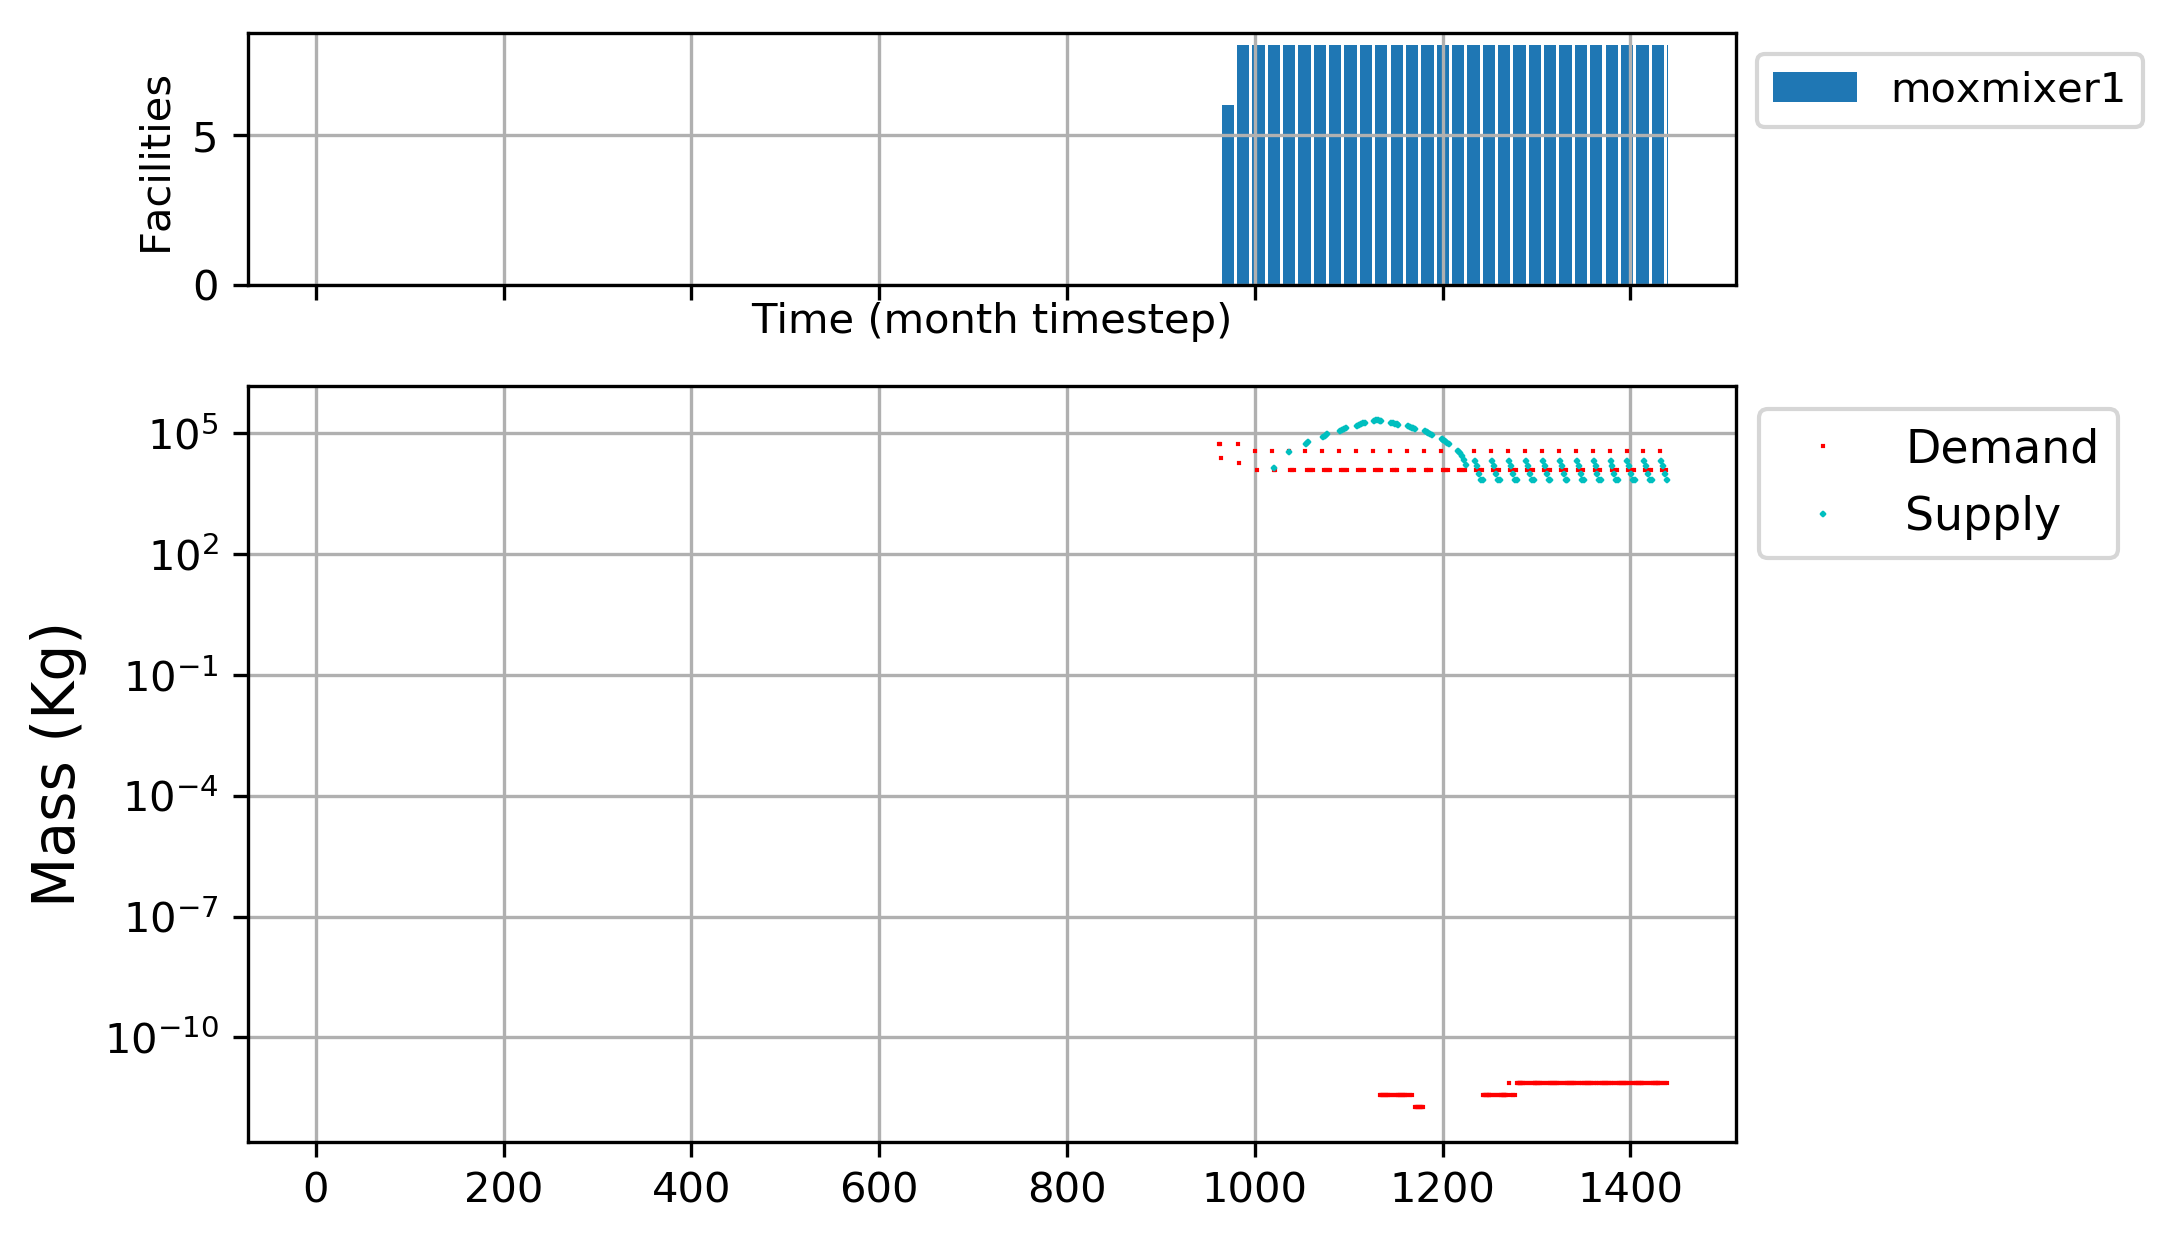
\includegraphics[width=\linewidth]{29-figures/0-poly-moxpu.png} 
		\caption{Commodity moxpu.}
		\label{fig:29-moxpu}
	\end{subfigure}
	\hfill
	\caption{Demand and supply of different commodities and number of facilities supplied with them.}
	\label{fig:29-pu2}
\end{figure}

\begin{table}[H]
	\centering
	\caption{Undersupply and oversupply of different commodities using poly to calculate EG01-EG29.}
	\label{tab:29-commod}
	\begin{tabularx}{\textwidth}{lRRR}
		\hline
		Commodity & Undersupplied & Cumulative  & Cumulative \\
		& Timesteps & Undersupply [$10^3$Kg]  & Oversupply [$10^6$Kg] \\ \hline
		Natural-U & 1 & 34394.0  & 132319869.5 \\ 
		Enriched-U & 1 & 16126.1 & 102751545581.6 \\
		FR Fuel & 2 & 284.4 & 124827.3 \\
        MOX LWR Fuel & 2 & 530.1 & 354541.5 \\ \hline
	\end{tabularx}
\end{table}

\section{Eg01-Eg30}

Figure \ref{fig:30flow} shows the facility and mass flow of transition scenario 
Eg01-Eg30 in \Cyclus.

\begin{figure}[H]
	\centering
	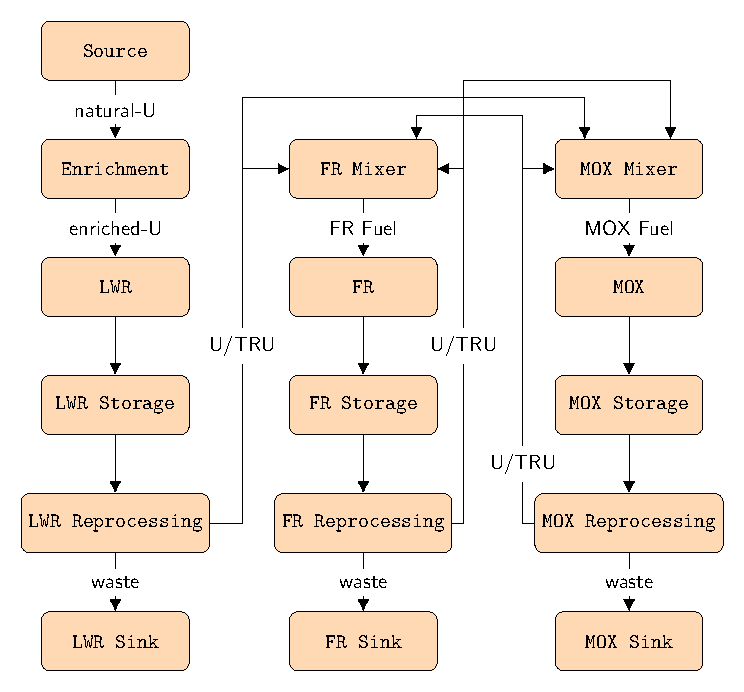
\includegraphics[width=0.8\textwidth]{30-figures/30flow.pdf} 
	\hfill
	\caption{Diagram with facilities and mass flow of the scenario EG01-EG30.}
	\label{fig:30flow}
\end{figure}

\subsection{Linearly increasing Power Demand: Power}

This section presents plots of power for all the prediction methods. 
The power demand increases linearly with the expression $60000 + 250t/12 MW$. 
Table \ref{tab:30-inputs} shows the input parameters. 
Figures \ref{fig:30-lin-NO}, \ref{fig:30-lin-DO}, and \ref{fig:30-lin-SO} 
display the power supply and demand. 
The plots only show the power demand and supply during the transition period. 
Undersupply of power occur during two main time periods:  
initial demand for the commodity and during the transition period. 
Undersupply time steps occurring at the beginning of the simulation 
is expected since without time series data at the beginning of the simulation, 
\deploy takes a few time steps to collect time series data about power demand 
to begin predicting and starting deployment of reactor and supporting fuel 
cycle facilities. 
Table \ref{tab:30-lin-power} records the number of steps of undersupply, 
the cumulative undersupply, and the cumulative oversupply. 
The smallest cumulative undersupply and smallest amount of undersupply 
time steps are for poly and fft prediction methods. 

\begin{table}[H]
	\centering
	\caption{EG01-EG30 input file values.}
	\label{tab:30-inputs}
	\begin{tabularx}{\textwidth}{lR}
		\hline
		Parameter			& Input \\ 	\hline
		Demand equation	[MW]	& 60000 + 250t/12  \\
		Deployment Driving Method 	& Installed Capacity \\
		Buffer    			& 0 \\
		Forward Steps		& 1 \\
		Backward Steps		& 2 \\		\hline
	\end{tabularx}
\end{table}

\begin{figure}[H]
	\centering
	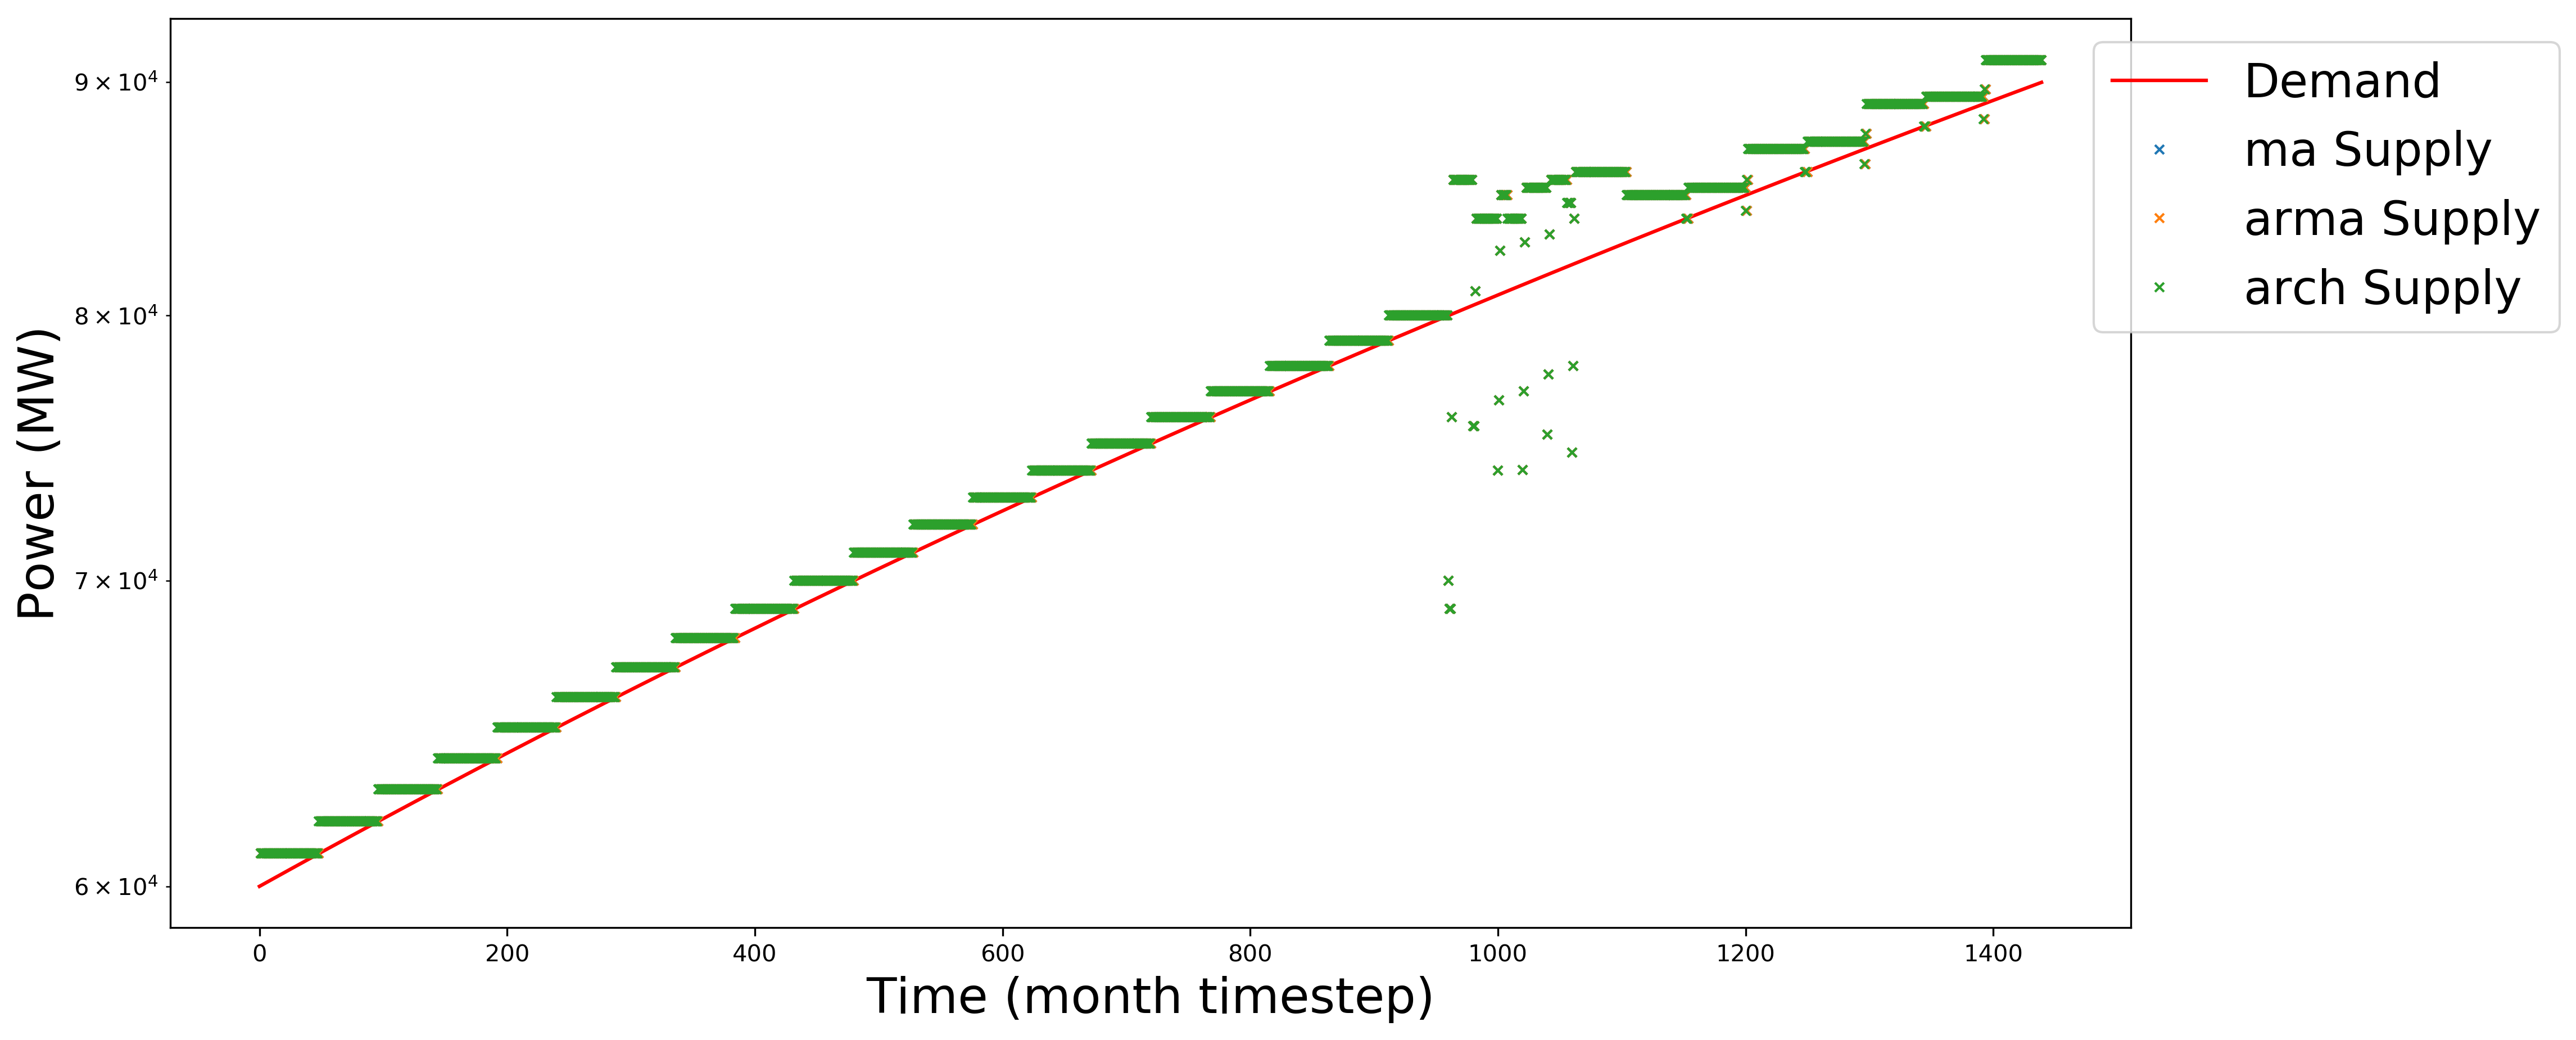
\includegraphics[width=\textwidth]{30-figures/lin-30-power-buffer01.png} 
	\hfill
	\caption{Linearly increasing power demand ($60000 + 250t/12 MW$) and power supply obtained with the NO algorithms.}
	\label{fig:30-lin-NO}
\end{figure}

\begin{figure}[H]
	\centering
	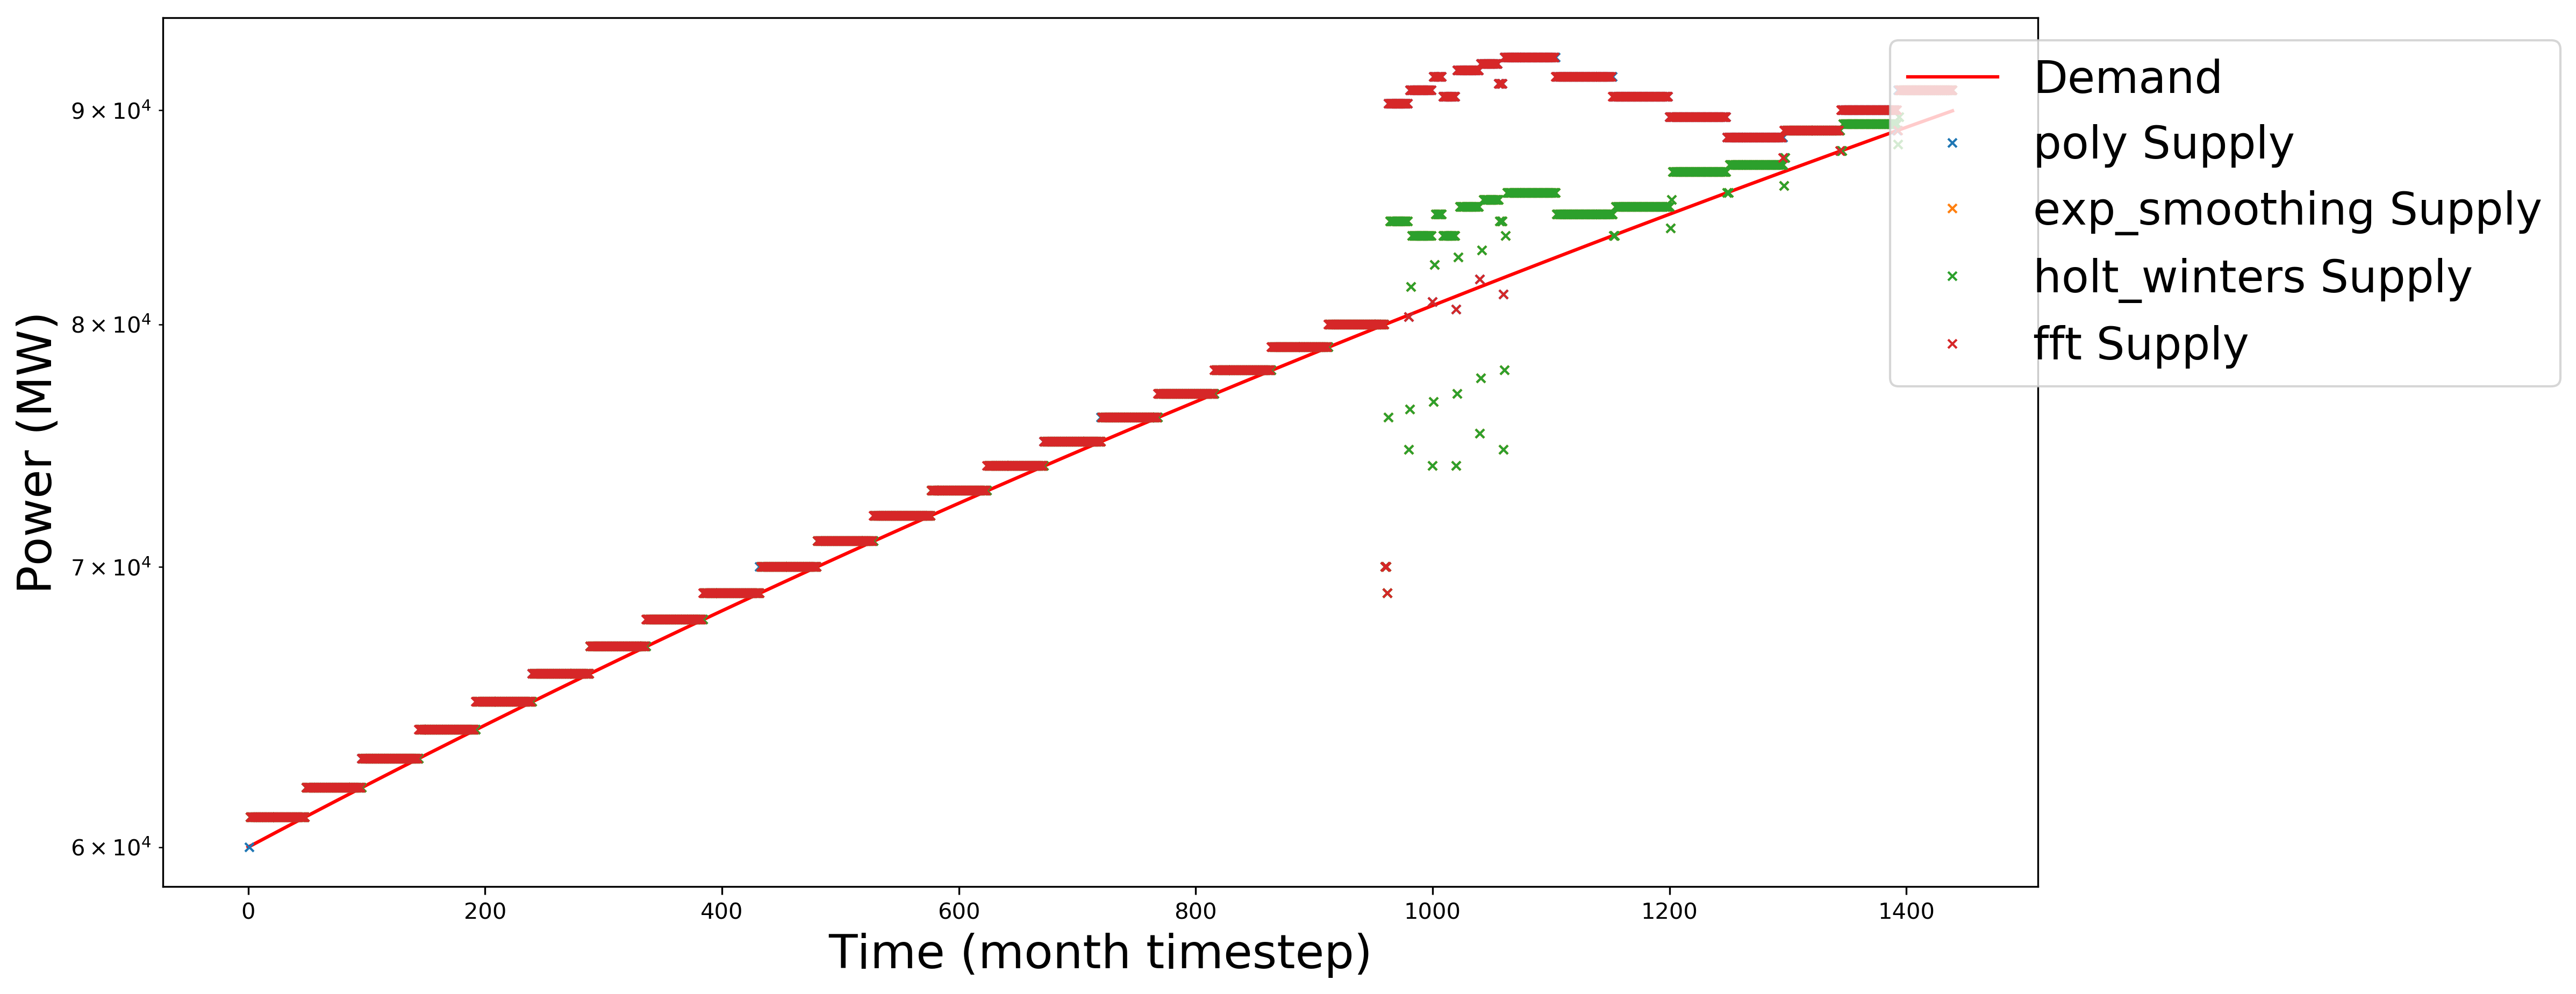
\includegraphics[width=\textwidth]{30-figures/lin-30-power-buffer02.png} 
	\hfill
	\caption{Linearly increasing power demand ($60000 + 250t/12 MW$) and power supply obtained with the DO algorithms.}
	\label{fig:30-lin-DO}
\end{figure}

\begin{figure}[H]
	\centering
	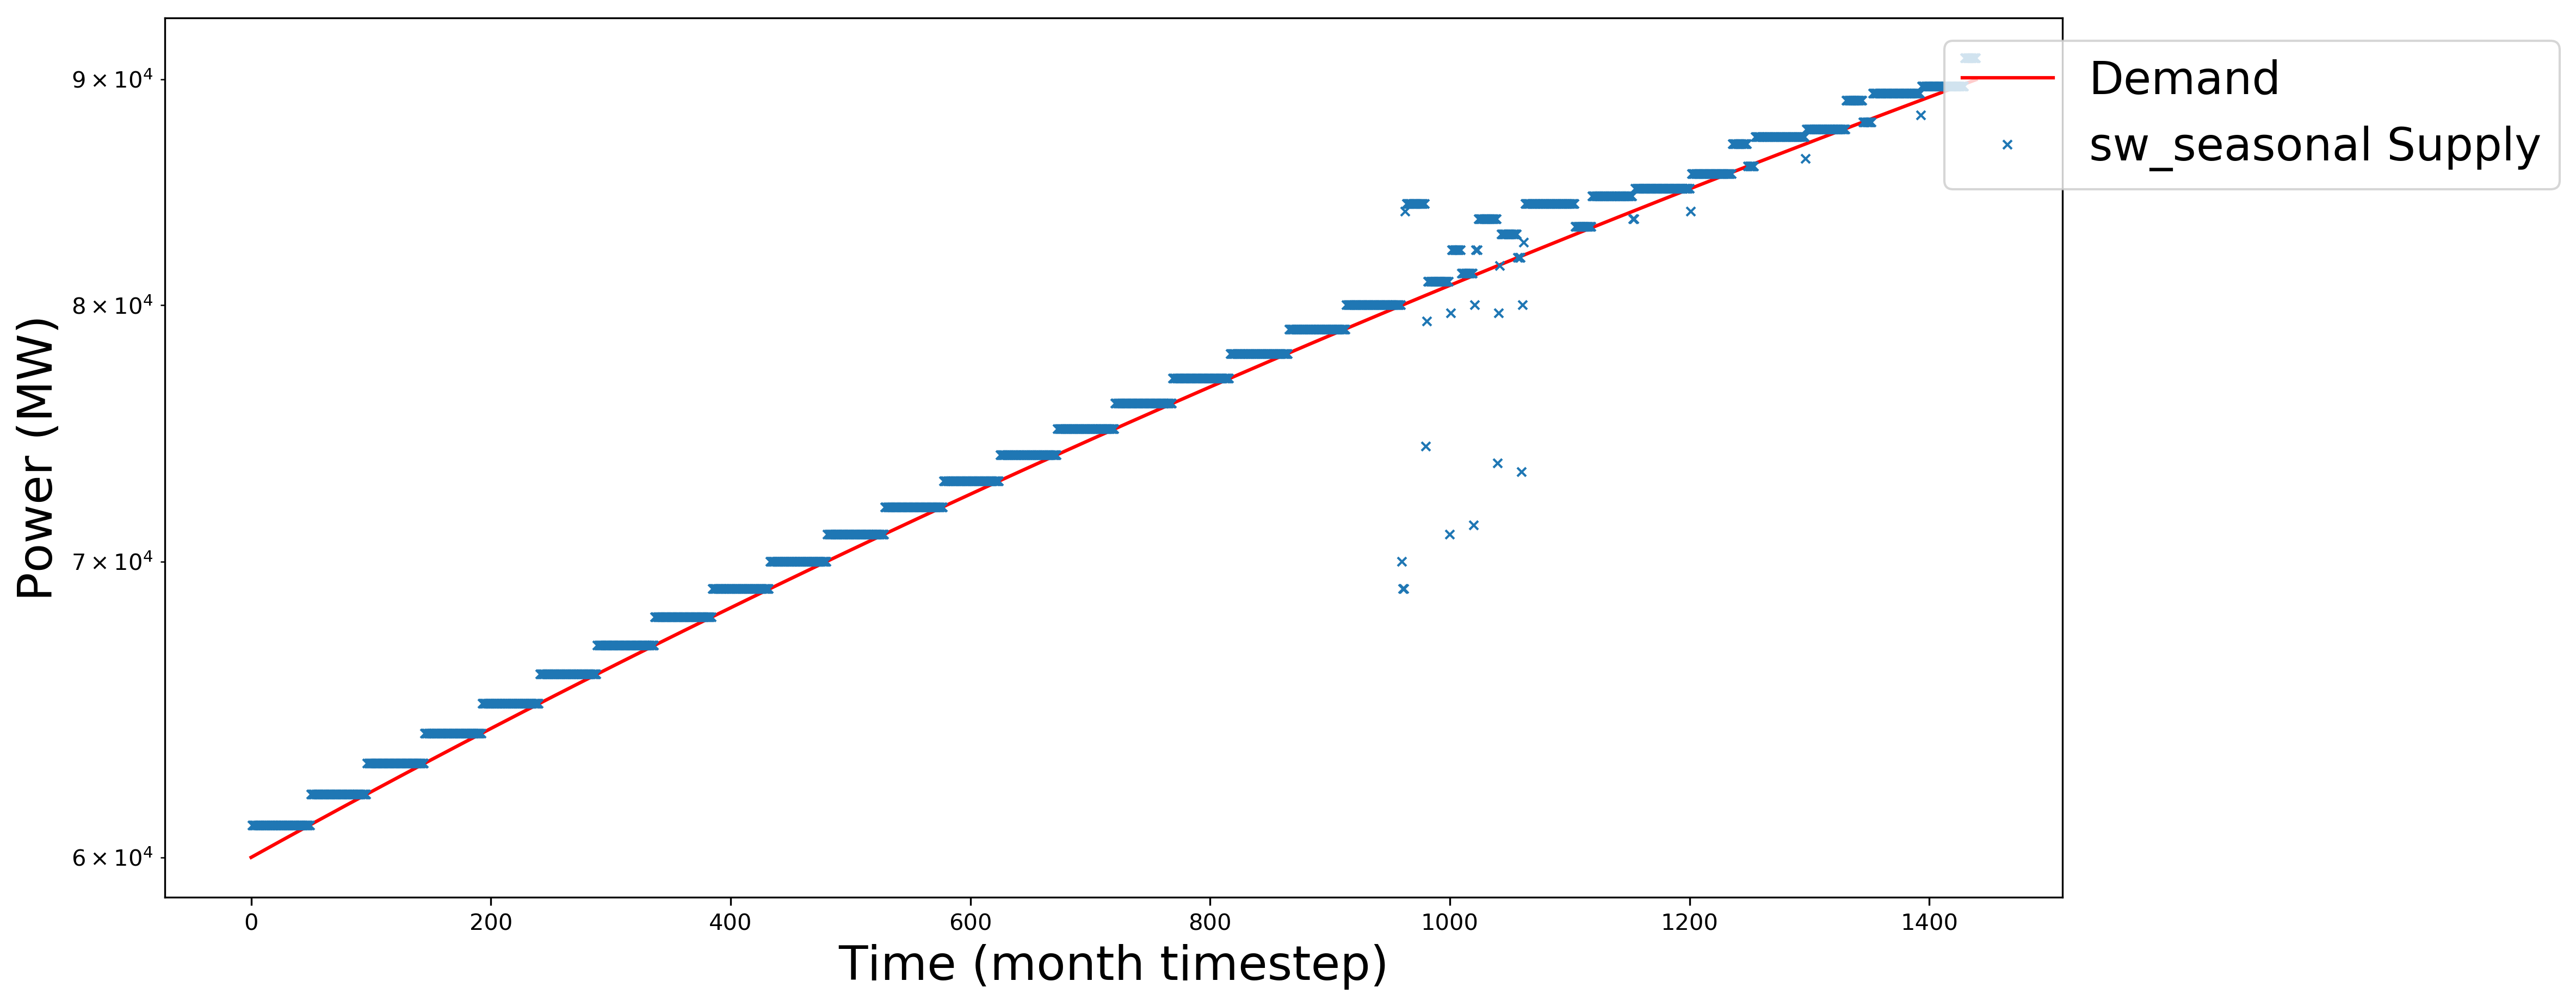
\includegraphics[width=\textwidth]{30-figures/lin-30-power-buffer03.png} 
	\hfill
	\caption{Linearly increasing power demand ($60000 + 250t/12 MW$) and power supply obtained with the SO algorithms.}
	\label{fig:30-lin-SO}
\end{figure}

\begin{table}[H]
	\centering
	\caption{Undersupply and oversupply of Power for the different prediction algorithms used to calculate EG01-EG24.}
	\label{tab:30-lin-power}
	\begin{tabularx}{\textwidth}{lRRR}
		\hline
		Algorithm & Undersupplied & Cumulative  & Cumulative \\
		& Timesteps     & Undersupply [GW.mo]  & Oversupply [GW.mo] \\ \hline
		MA        & 24 & 152.3 & 1334.1 \\ 
		ARMA      & 24 & 152.3 & 1334.1 \\ 
		ARCH      & 21 & 152.1 & 1355.9 \\ 
		POLY      &  9 & 92.5 & 3073.1 \\ 
		EXP\_SMOOTHING 	& 25 & 211.6 & 1317.8 \\ 
		HOLT-WINTERS  	& 25 & 211.6 & 1317.8 \\ 
		FFT       & 9 & 152.5 & 3079.4 \\ 
		SW\_SEASONAL  & 51 & 147.3 & 873.4 \\ \hline
	\end{tabularx}
\end{table}

\section{Summary}
By utilizing the sensitivity analysis and transition scenario set up in the previous 
sections, we determined the \deploy input parameters for EG01-EG23, EG01-EG24, EG01-EG29, 
and EG01-EG30 that minimize undersupply of power and minimize 
the undersupply and under capacity of the other commodities
in the simulation. 
Table \ref{tab:bestinputs} shows \deploy input parameters. 
The need for buffers for commodities is a reflection of reality
in which a supply buffer is usually maintained to ensure 
continuity in the event of an unexpected failure in the supply chain.

\begin{table}[]
	\resizebox{\textwidth}{!}{%
	\begin{tabular}{l|l|c|l|l|l}
	\hline
	\multirow{2}{*}{}                         & \multicolumn{1}{c|}{\multirow{2}{*}{\textbf{Input Parameter}}} & \multicolumn{4}{c}{\textbf{Simulation Description}}                                                                                                                                                                                                                                                       \\ \cline{3-6} 
											  & \multicolumn{1}{c|}{}                                          & \multicolumn{1}{l|}{\textbf{EG01-23}}                                                                 & \textbf{EG01-24}                  & \textbf{EG01-29}                 &\textbf{EG01-30}                                                  \\ \hline
	\multirow{4}{*}{\textbf{Required}} & Demand driving commodity                                       & \multicolumn{4}{c}{Power}                                                                                                                                                                                                                                                                                 \\ \cline{2-6} 
											  & Demand equation [MW]                                               & \multicolumn{1}{l|}{60000}                                                                                & $60000 + 250t/12$ & 60000                     &     $60000 + 250t/12$                                       \\ \cline{2-6} 
											  & Prediction method                                              & \texttt{poly}       & \texttt{fft}             & \texttt{poly}         &  \texttt{fft}    \\ \cline{2-6} 
											  & Deployment Driving Method                                      & \multicolumn{4}{c}{Installed Capacity}                                                                                                                                                                                                                                                                    \\ \hline
	\multirow{2}{*}{\textbf{Optional}} & Buffer type                                                    & \multicolumn{4}{c}{Absolute}                                                                                                                                                                                                                                                               \\ \cline{2-6} 
											  & Power Buffer size [MW]                                                   & 0 & 6000 & 0 & 8000 \\ \hline
	\end{tabular}%
	}
	\caption{\deploy's input parameters for EG01-EG23, EG01-EG24, EG01-EG29, and 
	EG01-EG30 transition scenarios
	that minimizes undersupply of power and minimizes 
	the undersupply and under capacity of the other facilities. }
	\label{tab:bestinputs}
	\end{table}

Figures \ref{fig:23stack}, \ref{fig:24stack}, \ref{fig:29stack}, 
and \ref{fig:30stack} show
time dependent deployment of reactor and supporting facilities for 
the EG01-23 constant power demand, EG01-24 linearly increasing power demand, 
EG01-29 constant power demand, EG01-30 linearly increasing power demand
transition scenarios, respectively. 
\deploy automatically deploys reactor and supporting facilities 
to setup a supply chain to meet power demand
during a transition from \glspl{LWR} to \glspl{SFR} for EG01-23 and EG01-24, 
and from \glspl{LWR} to \gls{MOX} \glspl{LWR} and \glspl{SFR} for EG01-29 and
EG01-30. 

\begin{figure}[]
	\centering
	\begin{subfigure}[t]{1.2\textwidth}
		\centering
		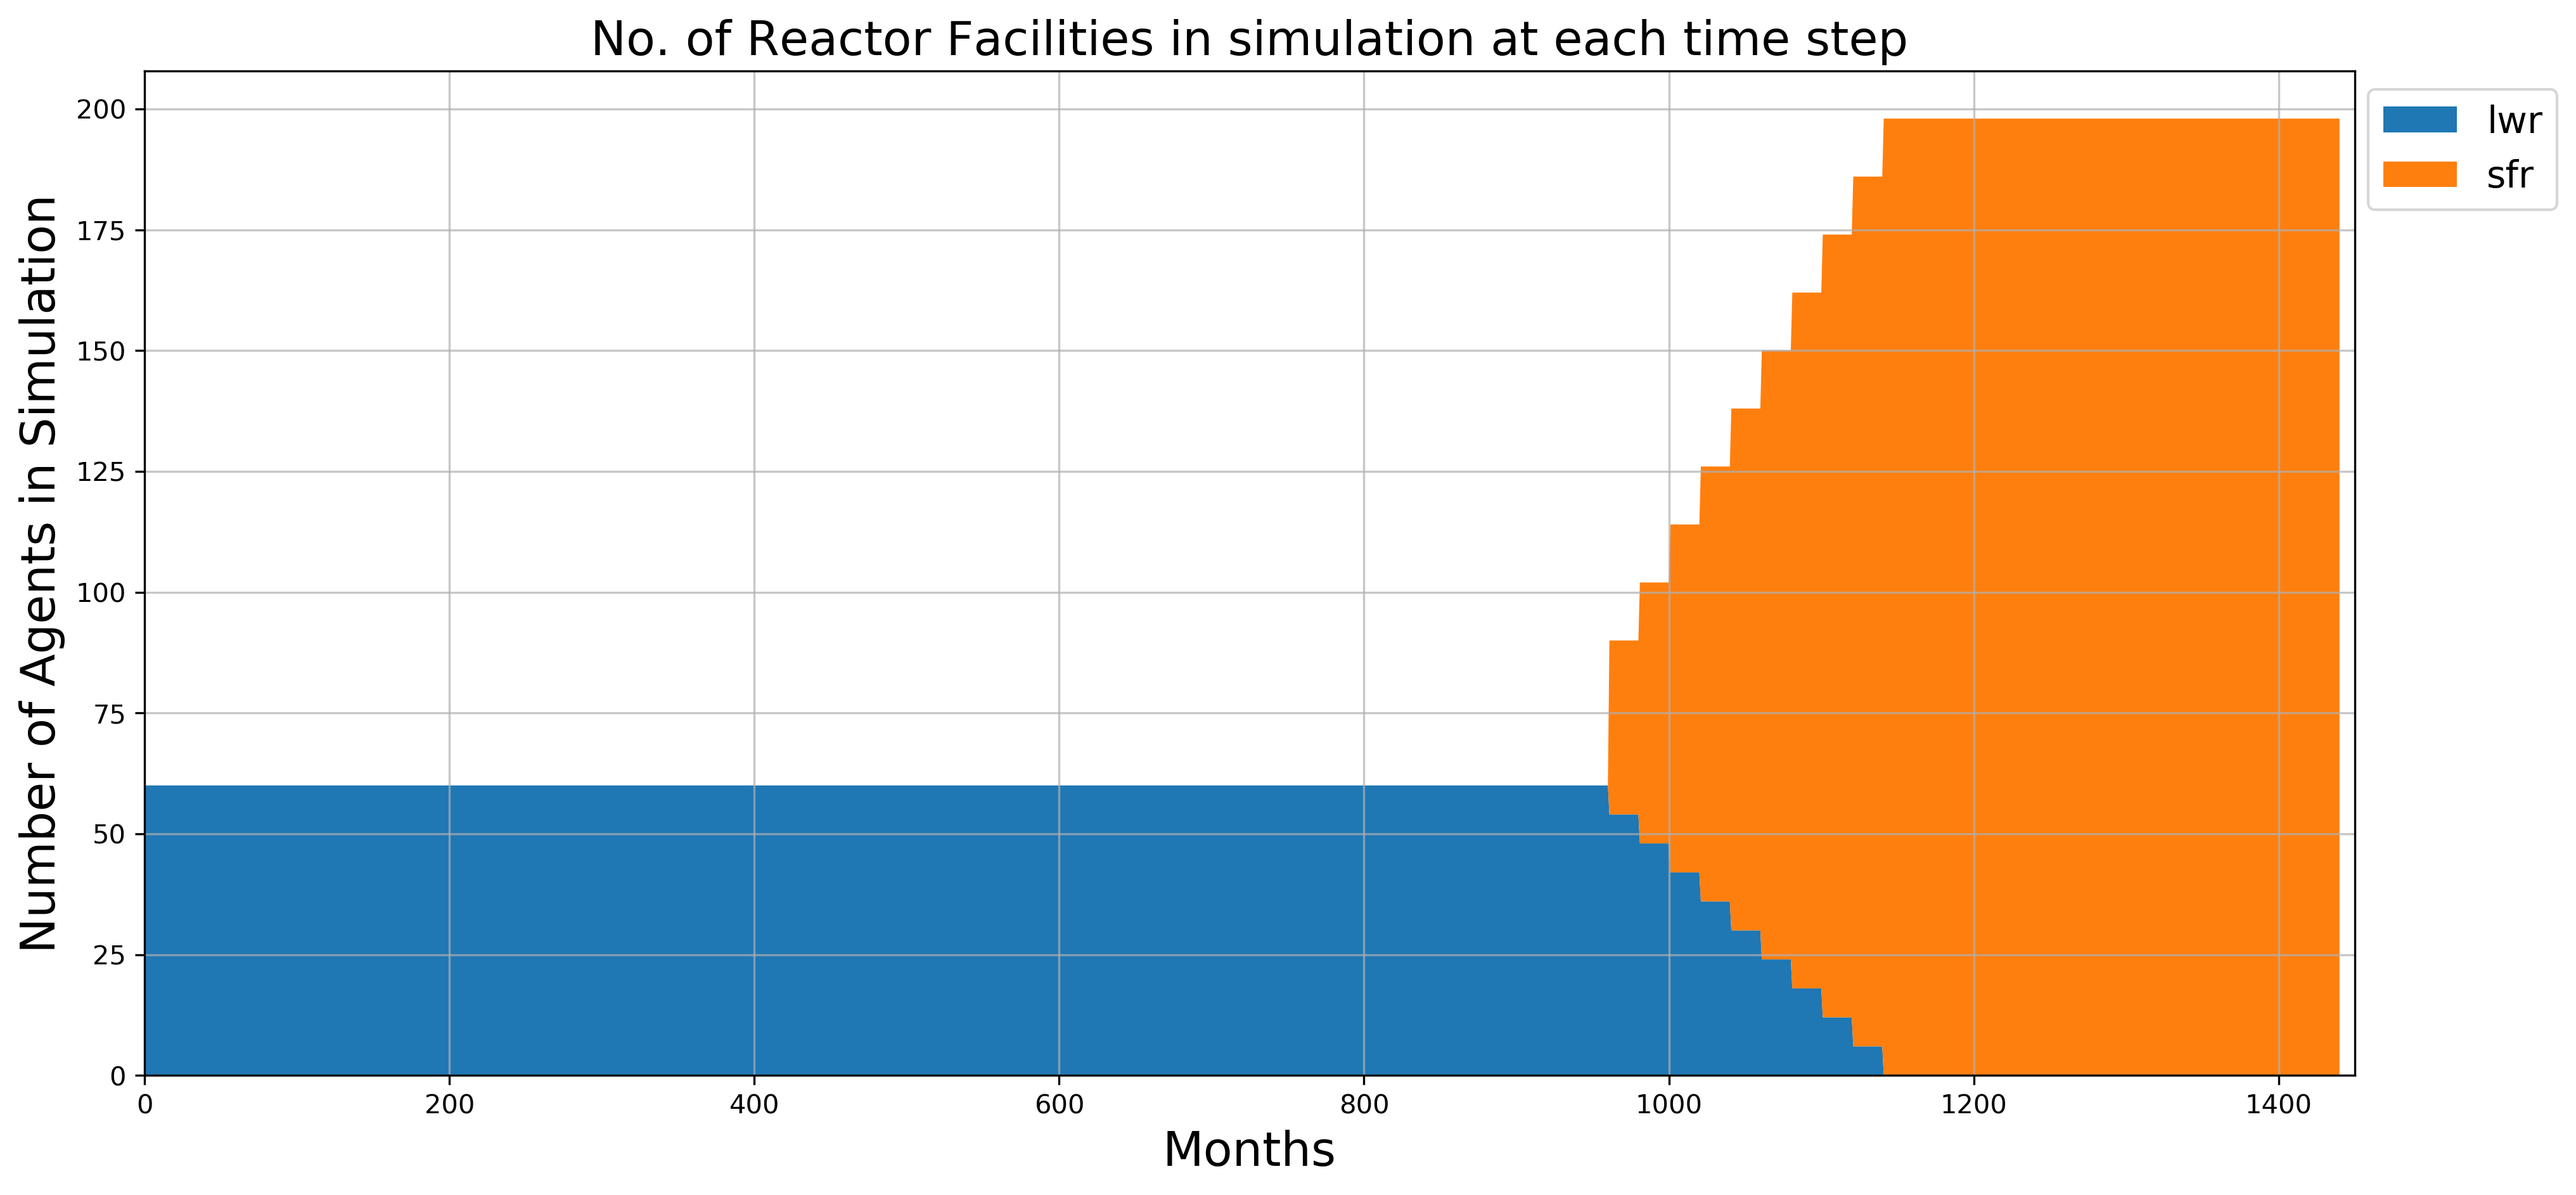
\includegraphics[width=\linewidth]{23-figures/eg23-stack_reactor.png} 
		\caption{EG01-23: Reactor Deployment}
		\label{fig:23reactor}
	\end{subfigure}
	\vspace{1cm}
	\begin{subfigure}[t]{1.2\textwidth}
		\centering
		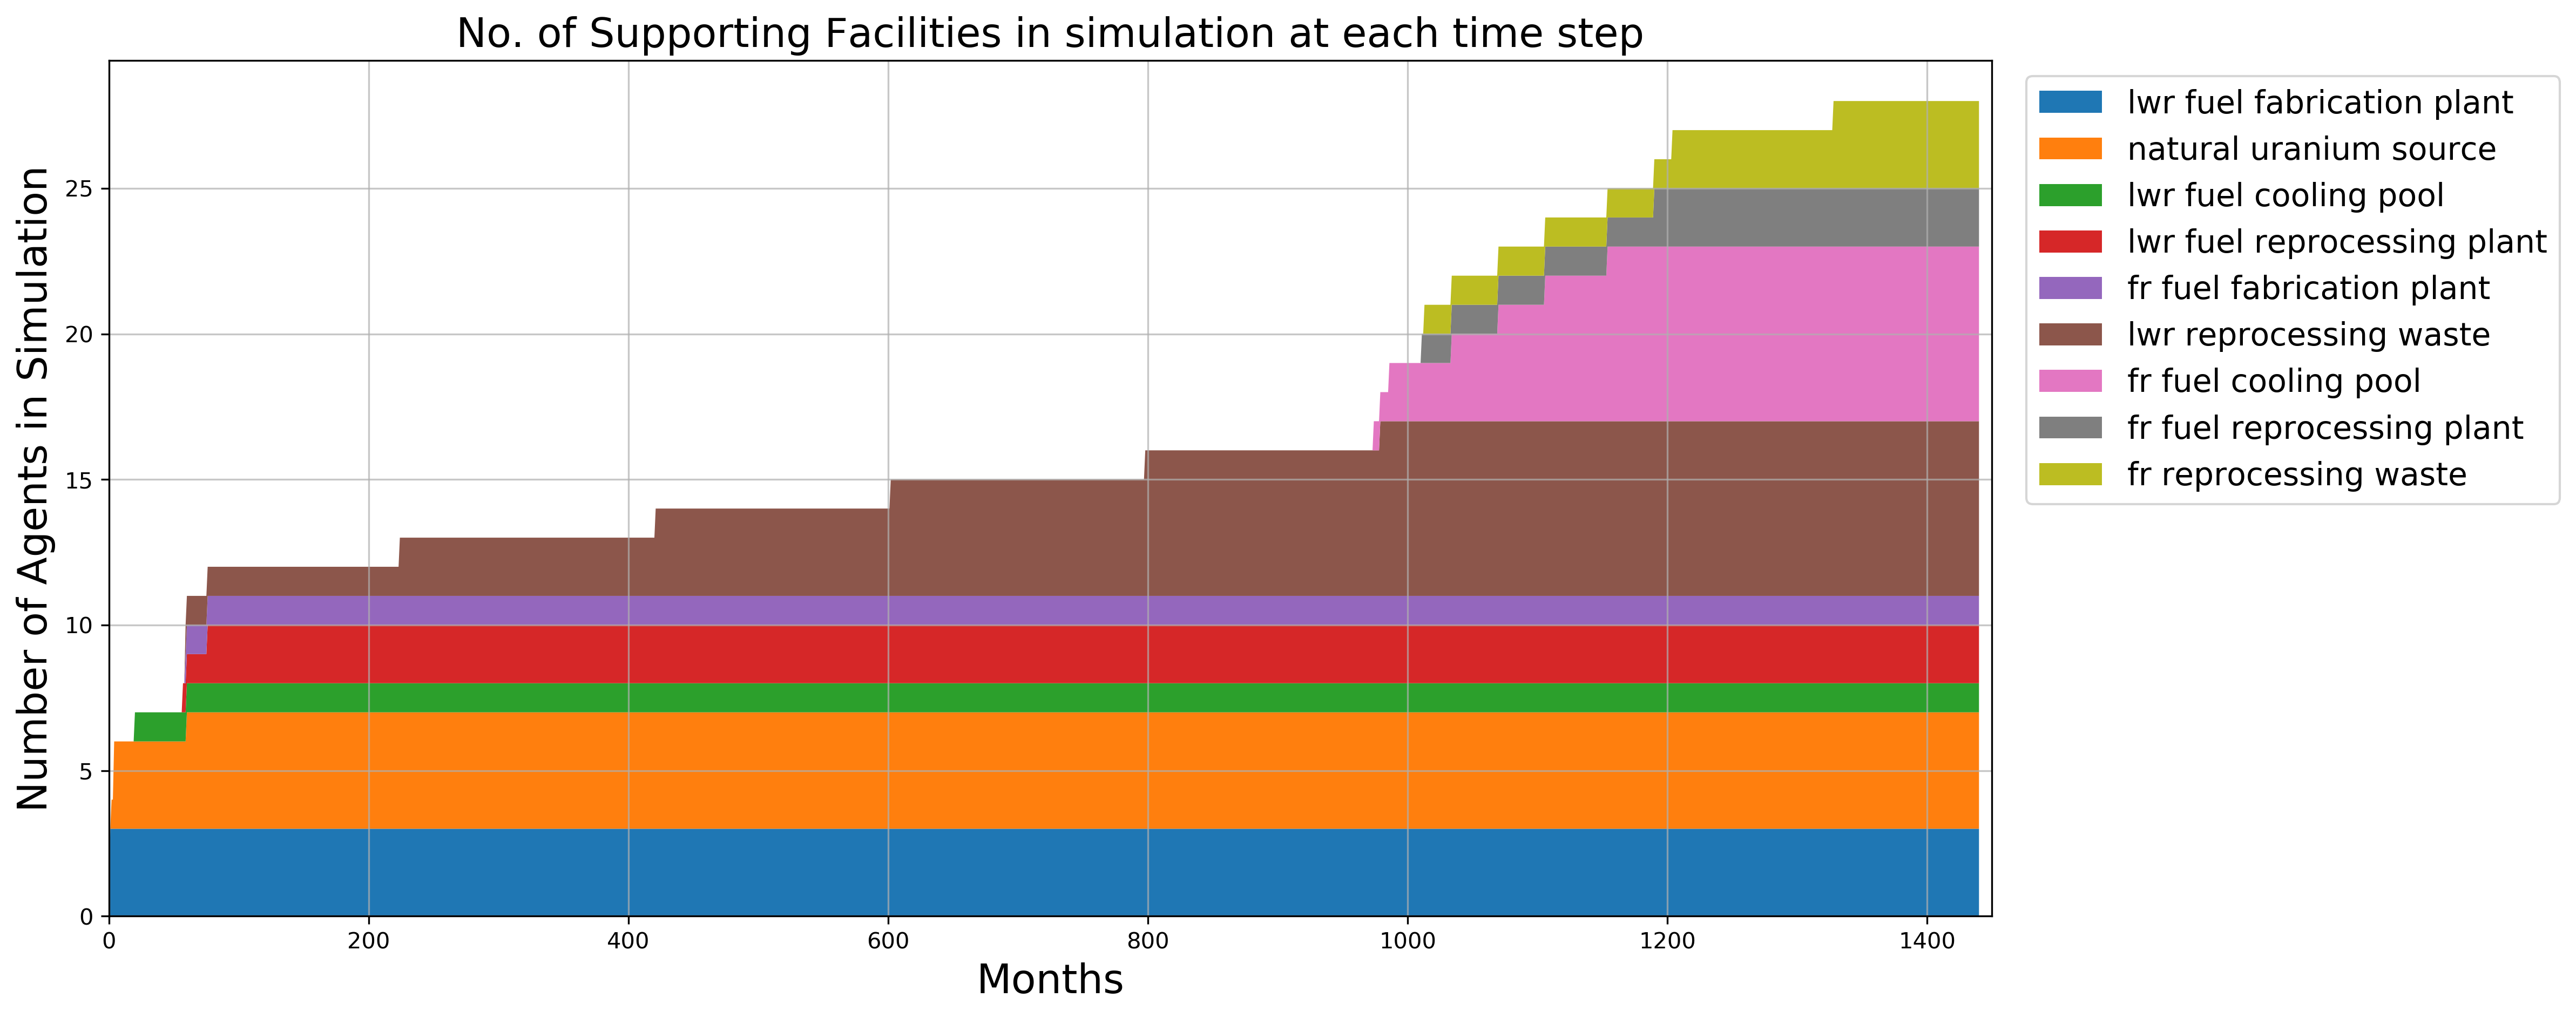
\includegraphics[width=\linewidth]{23-figures/eg23-stack_support.png} 
		\caption{EG01-23: Supporting Facility Deployment}
		\label{fig:23support}
	\end{subfigure}
	\hfill
	\caption{Time dependent deployment of reactor and supporting facilities in 
	the EG01-23 constant power demand transition scenario. 
	\deploy automatically deploys reactor and supporting facilities 
	to setup a supply chain to meet constant power demand of $60000$ MW
	during a transition from \glspl{LWR} to \glspl{SFR}. }
	\label{fig:23stack}
\end{figure}

\begin{figure}[]
	\centering
	\begin{subfigure}[t]{1.2\textwidth}
		\centering
		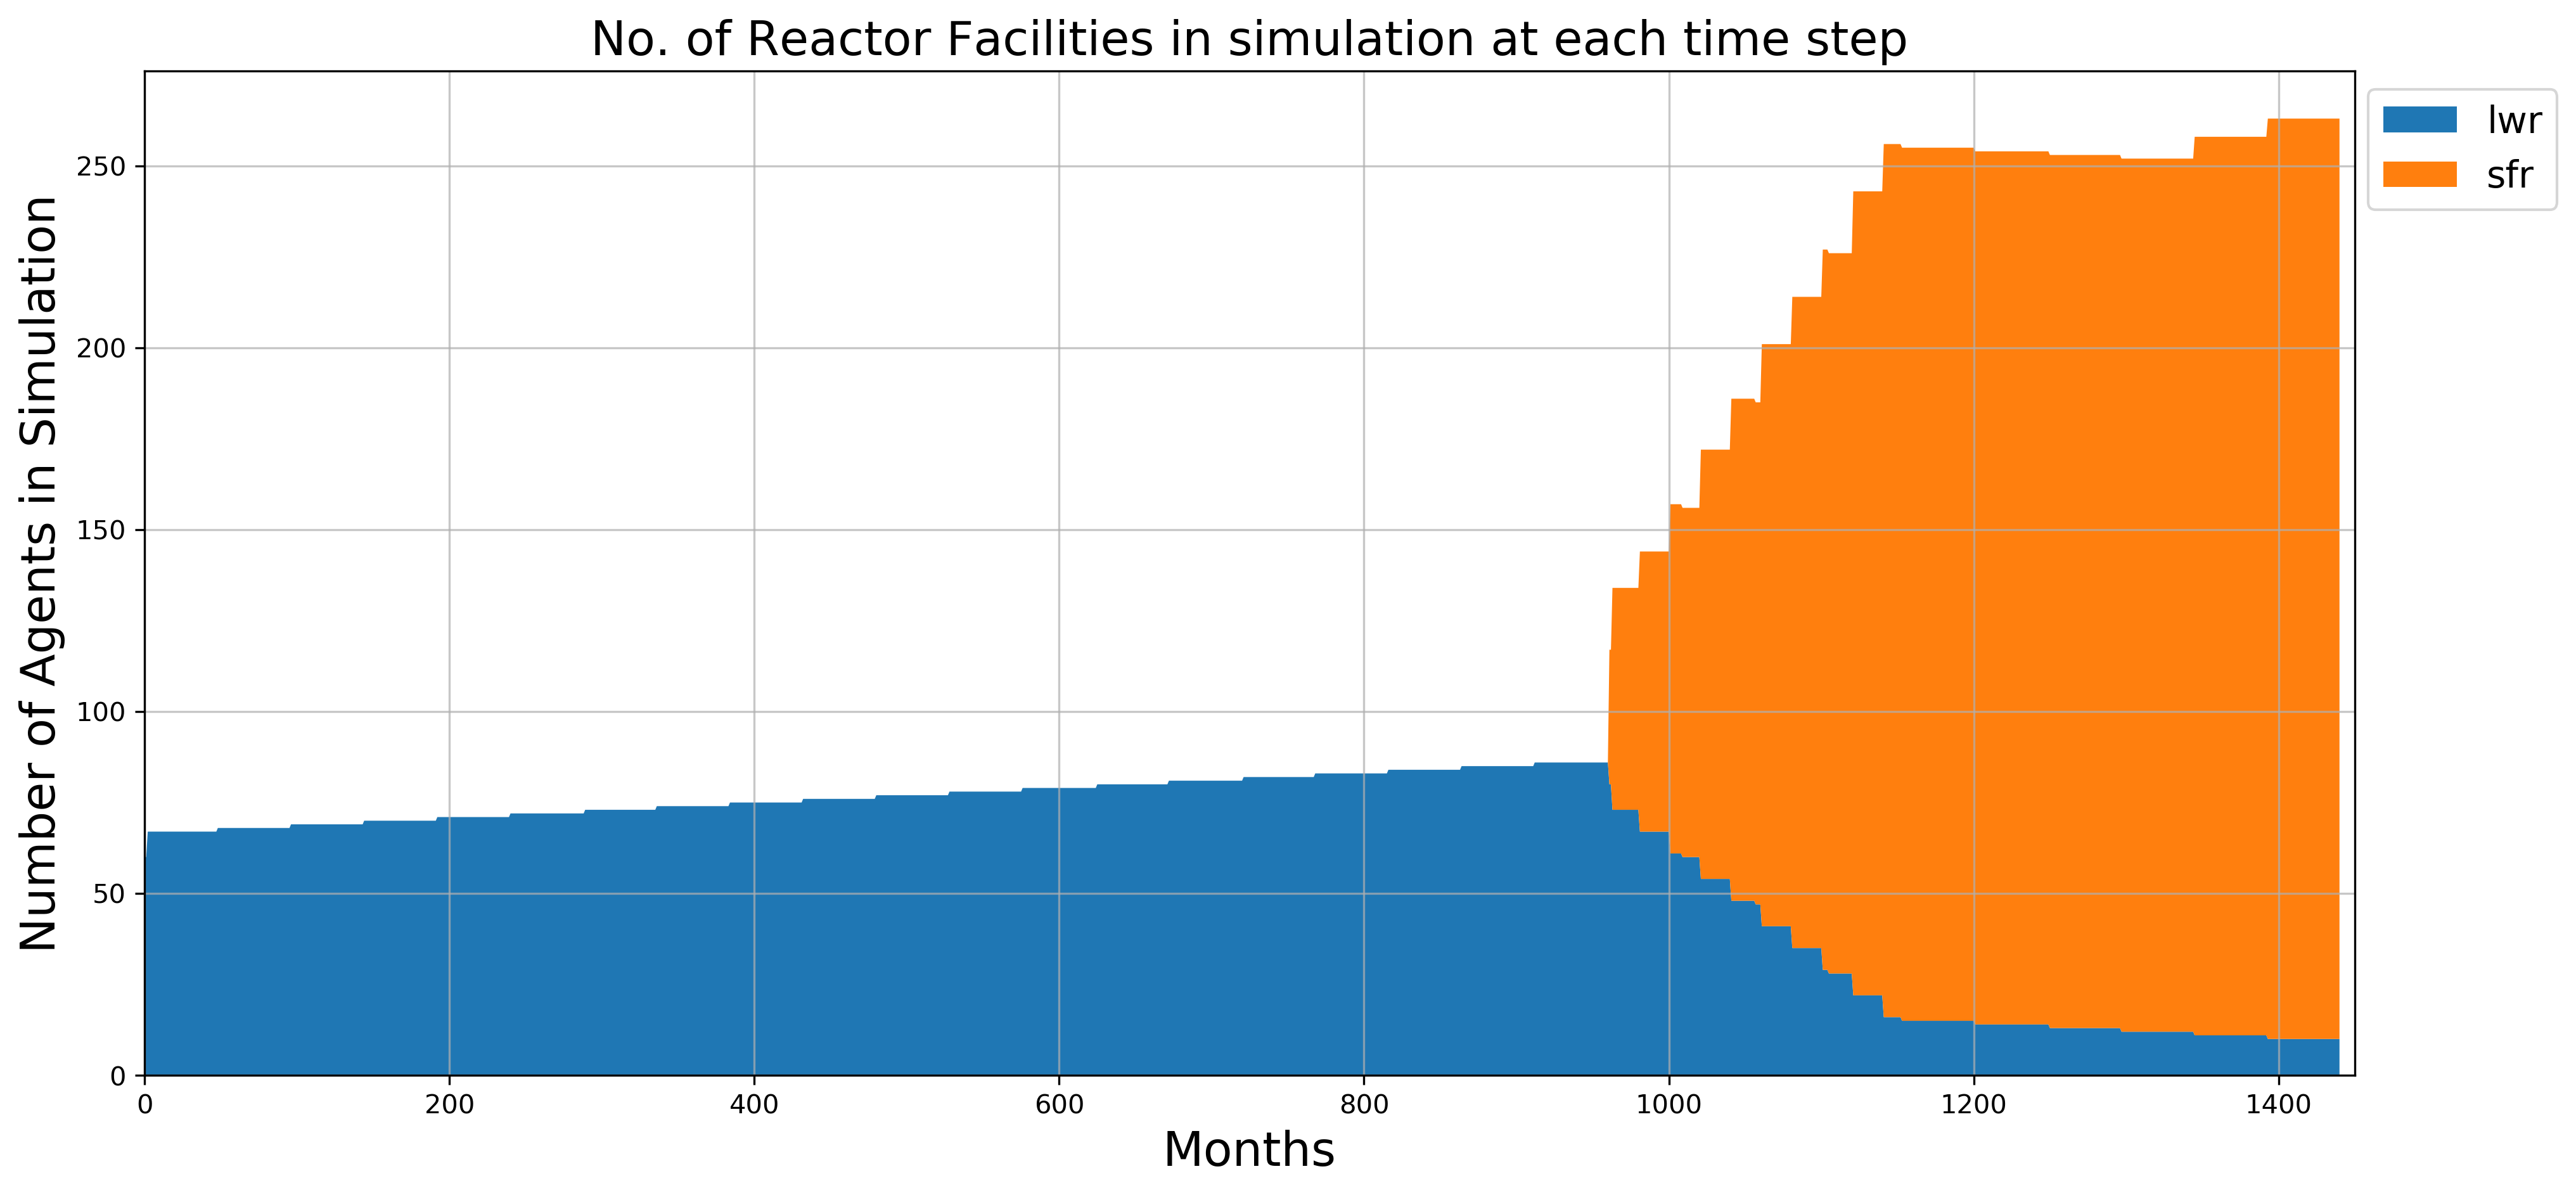
\includegraphics[width=\linewidth]{24-figures/eg24-stack_reactor.png} 
		\caption{EG01-24: Reactor Deployment}
		\label{fig:24reactor}
	\end{subfigure}
	\vspace{1cm}
	\begin{subfigure}[t]{1.2\textwidth}
		\centering
		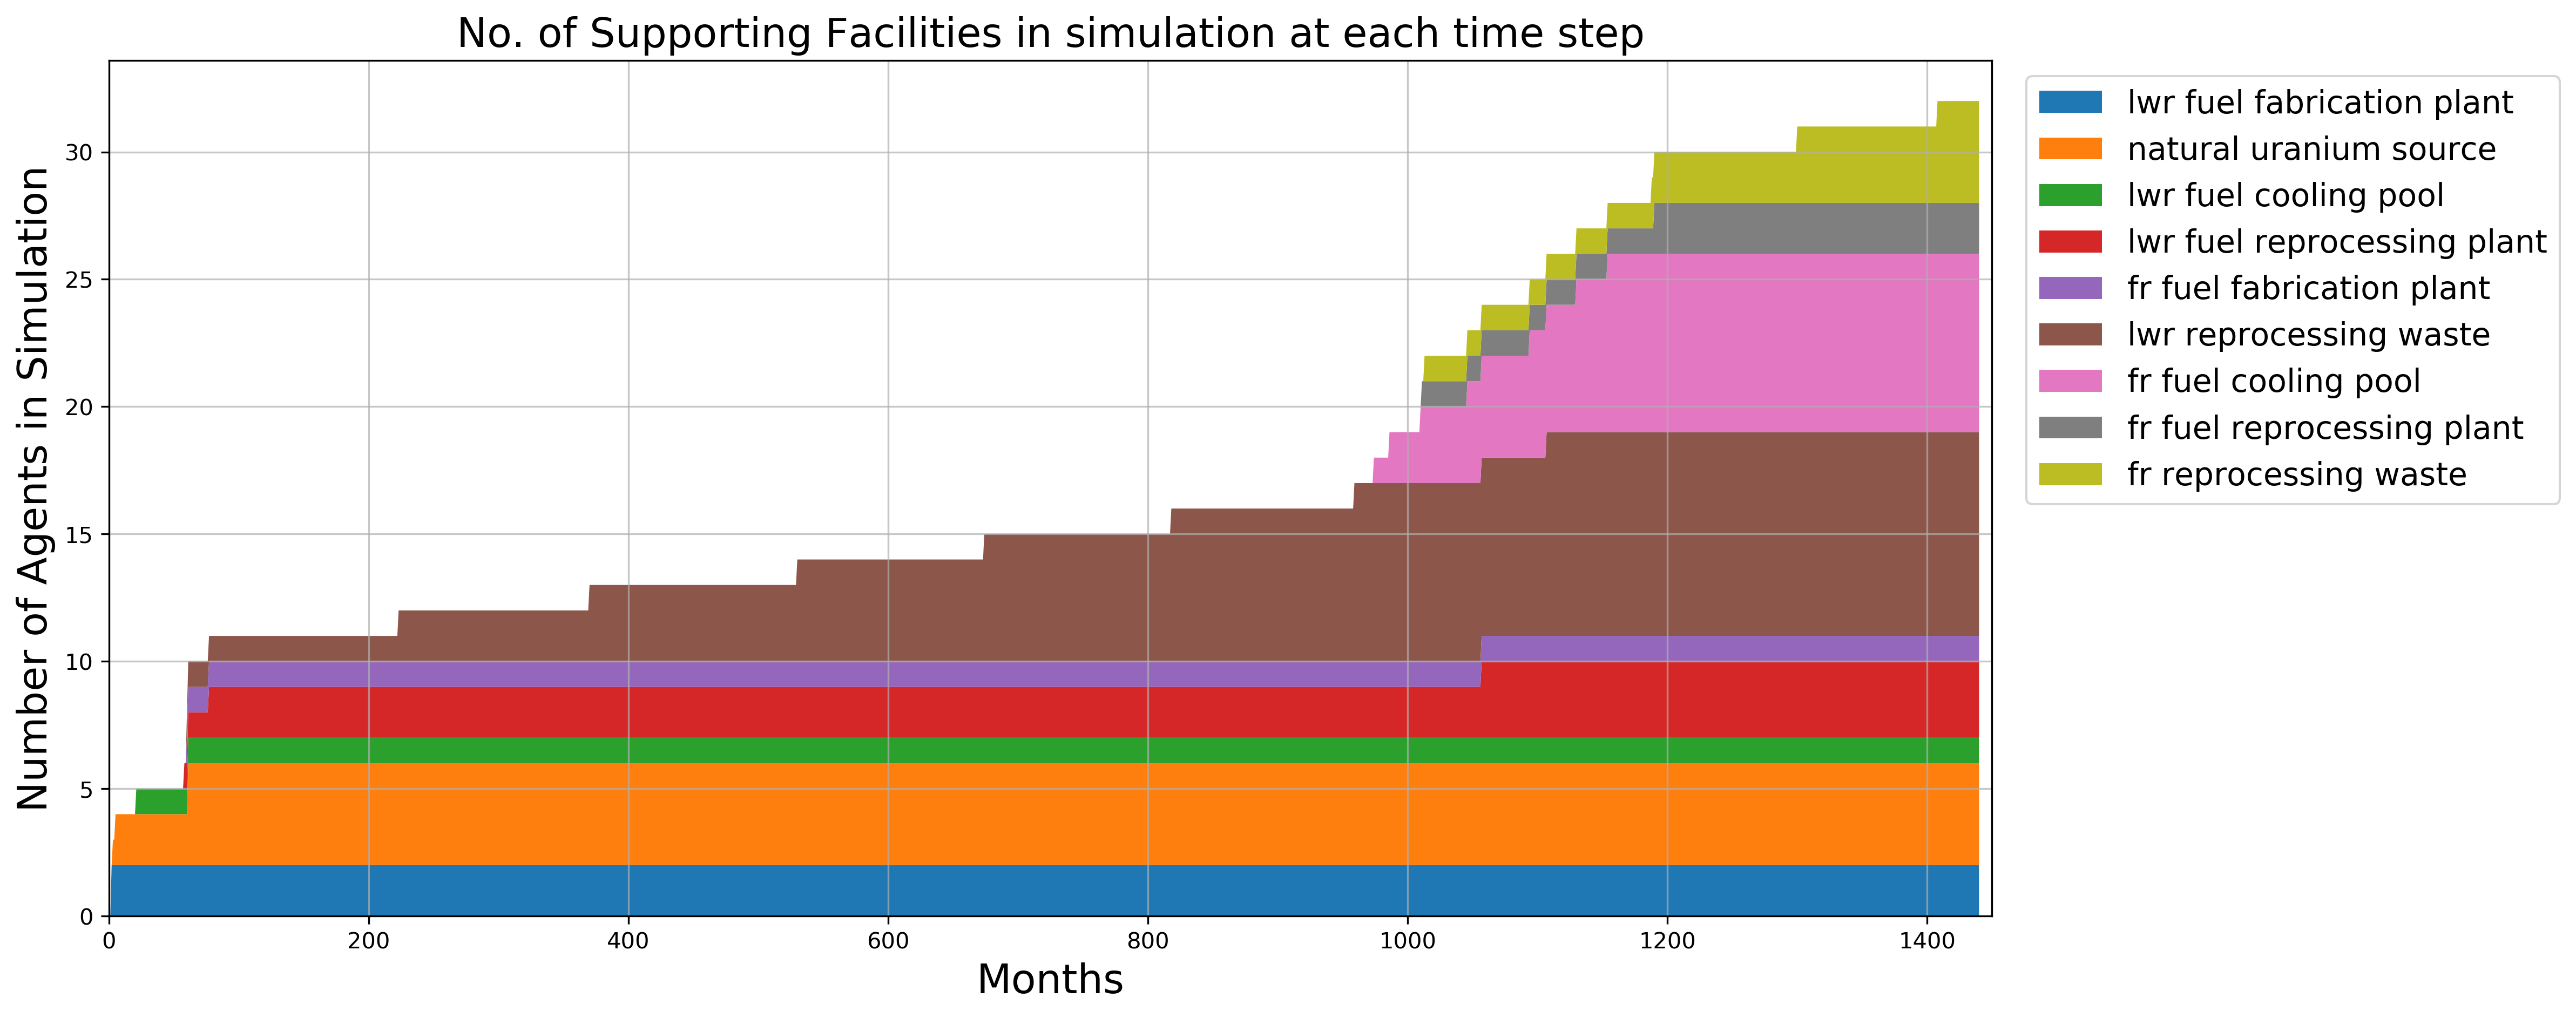
\includegraphics[width=\linewidth]{24-figures/eg24-stack_support.png} 
		\caption{EG01-24: Supporting Facility Deployment}
		\label{fig:24support}
	\end{subfigure}
	\hfill
	\caption{Time dependent deployment of reactor and supporting facilities in 
	the EG01-24 linearly increasing power demand transition scenario. 
	\deploy automatically deploys reactor and supporting facilities 
	to setup a supply chain to meet linearly increasing power demand of $60000 + 250t/12$ MW
	during a transition from \glspl{LWR} to \glspl{SFR}. }
	\label{fig:24stack}
\end{figure}

\begin{figure}[]
	\centering
	\begin{subfigure}[t]{1.2\textwidth}
		\centering
		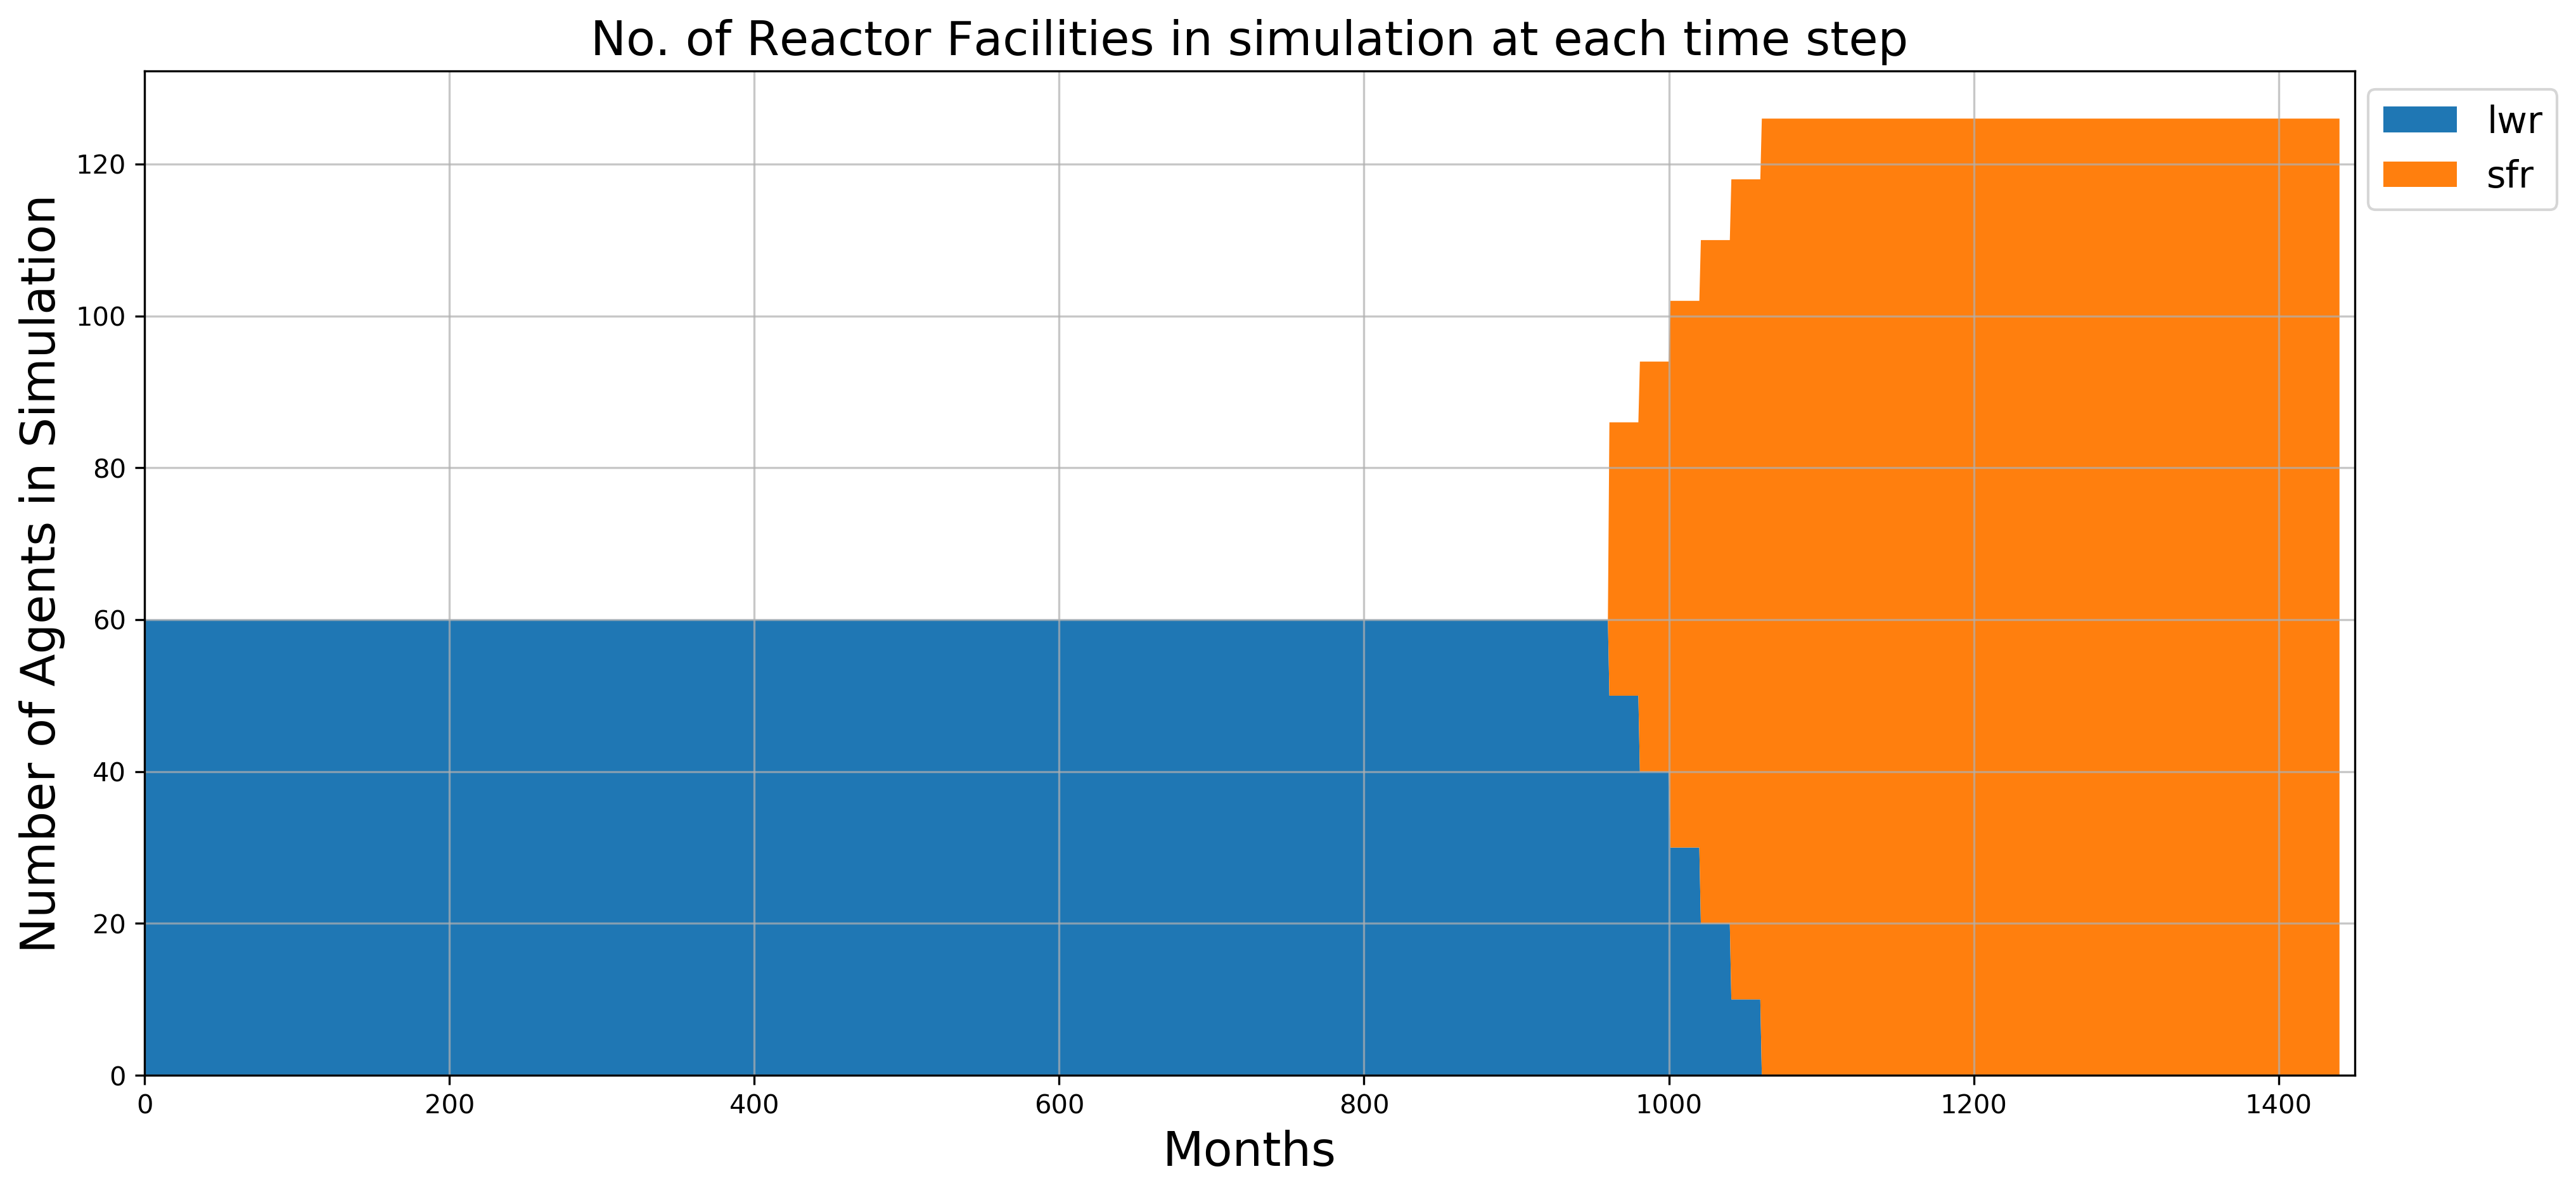
\includegraphics[width=\linewidth]{29-figures/eg29-stack_reactor.png} 
		\caption{EG01-29: Reactor Deployment}
		\label{fig:29reactor}
	\end{subfigure}
	\vspace{1cm}
	\begin{subfigure}[t]{1.2\textwidth}
		\centering
		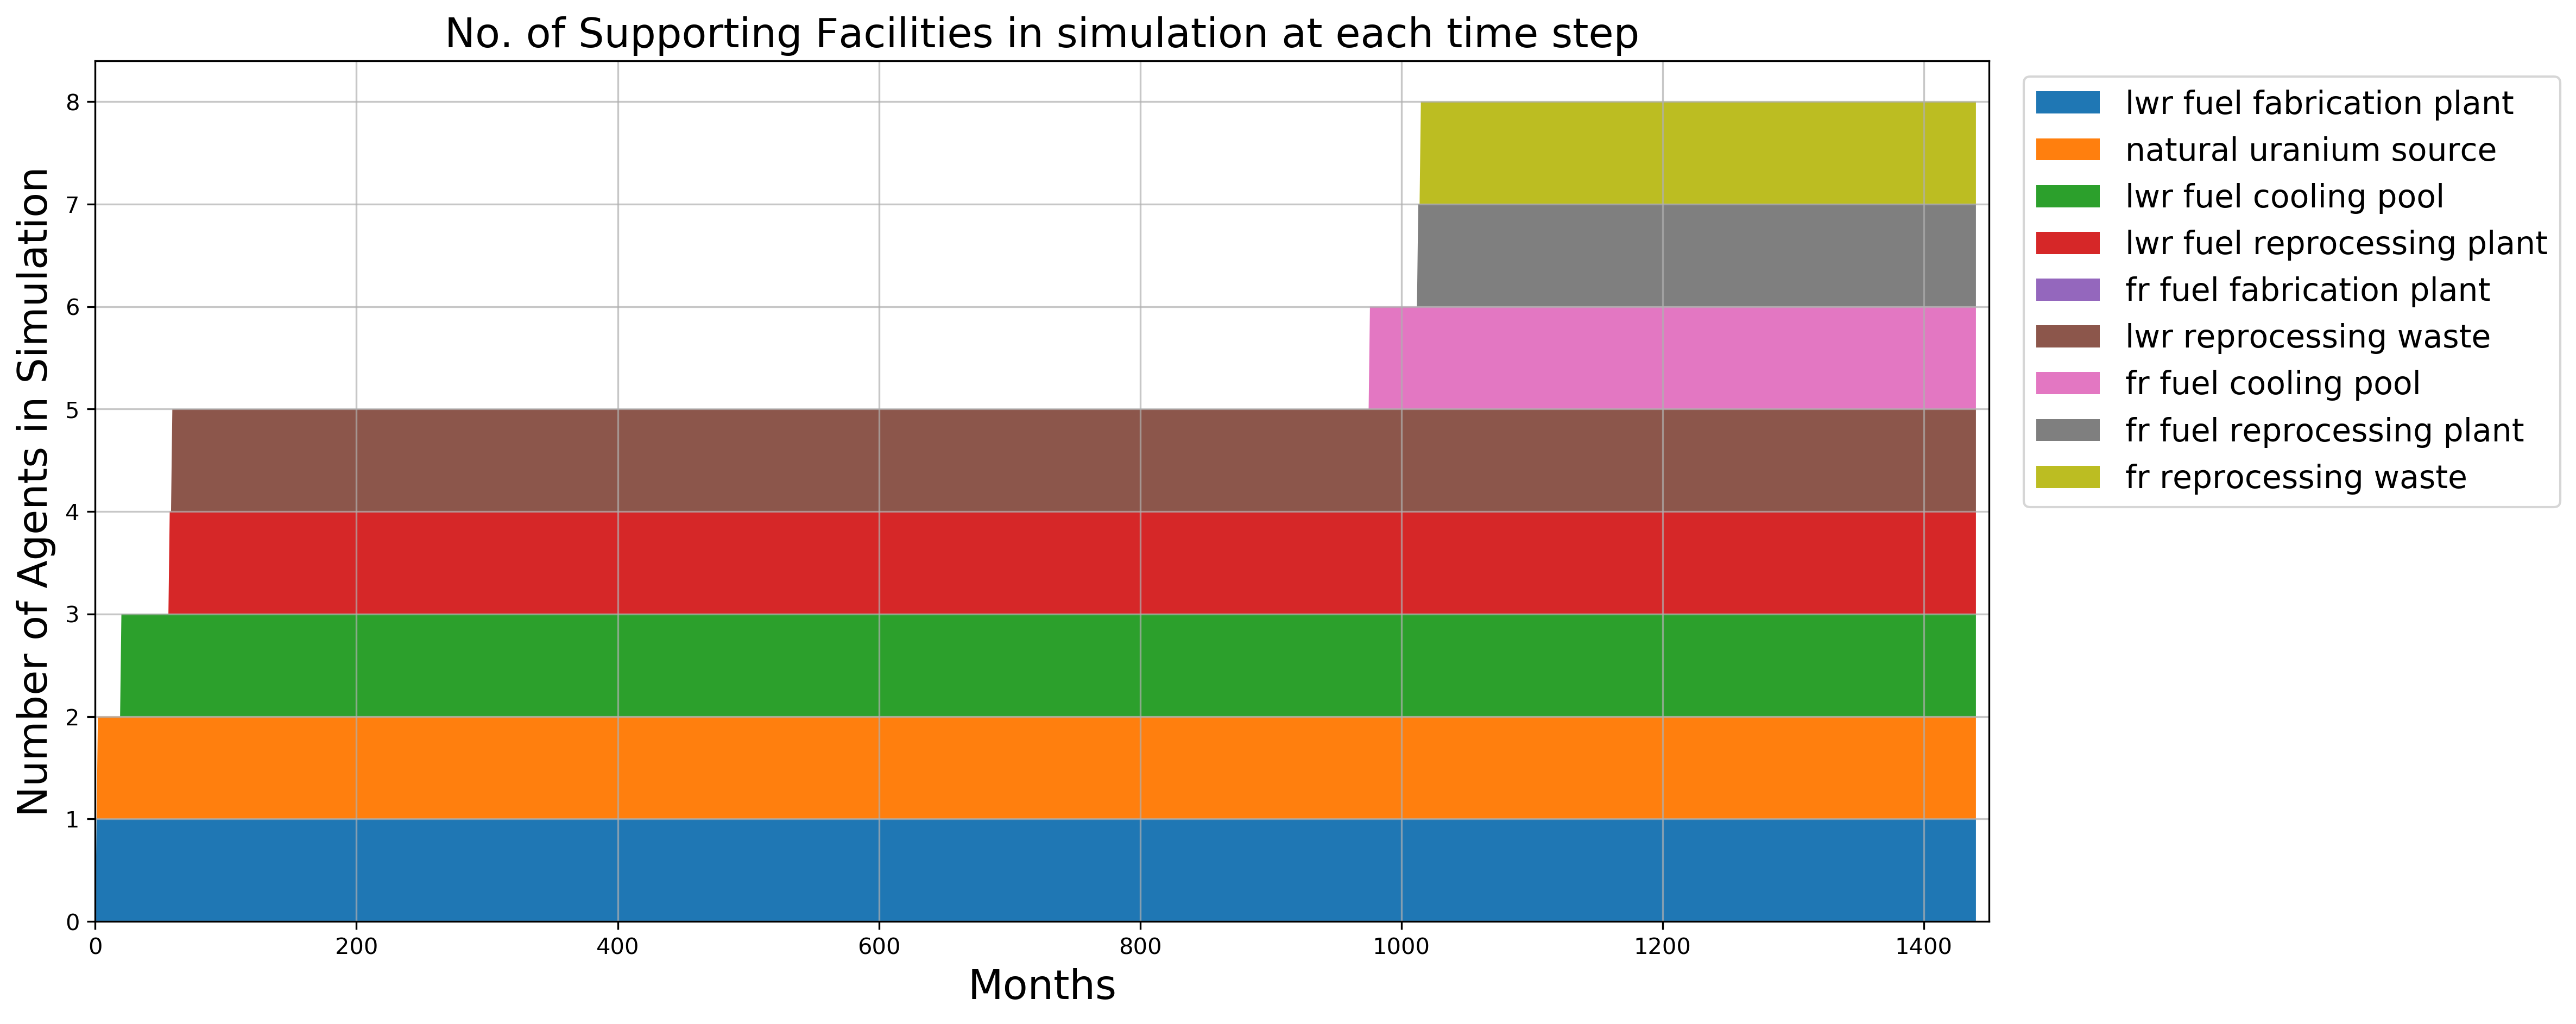
\includegraphics[width=\linewidth]{29-figures/eg29-stack_support.png} 
		\caption{EG01-29: Supporting Facility Deployment}
		\label{fig:29support}
	\end{subfigure}
	\hfill
	\caption{Time dependent deployment of reactor and supporting facilities in 
	the EG01-29 linearly increasing power demand transition scenario. 
	\deploy automatically deploys reactor and supporting facilities 
	to setup a supply chain to meet constant power demand of $60000$ MW
	during a transition from \glspl{LWR} to MOX LWRs and \glspl{SFR}. }
	\label{fig:29stack}
\end{figure}

\begin{figure}[]
	\centering
	\begin{subfigure}[t]{1.2\textwidth}
		\centering
		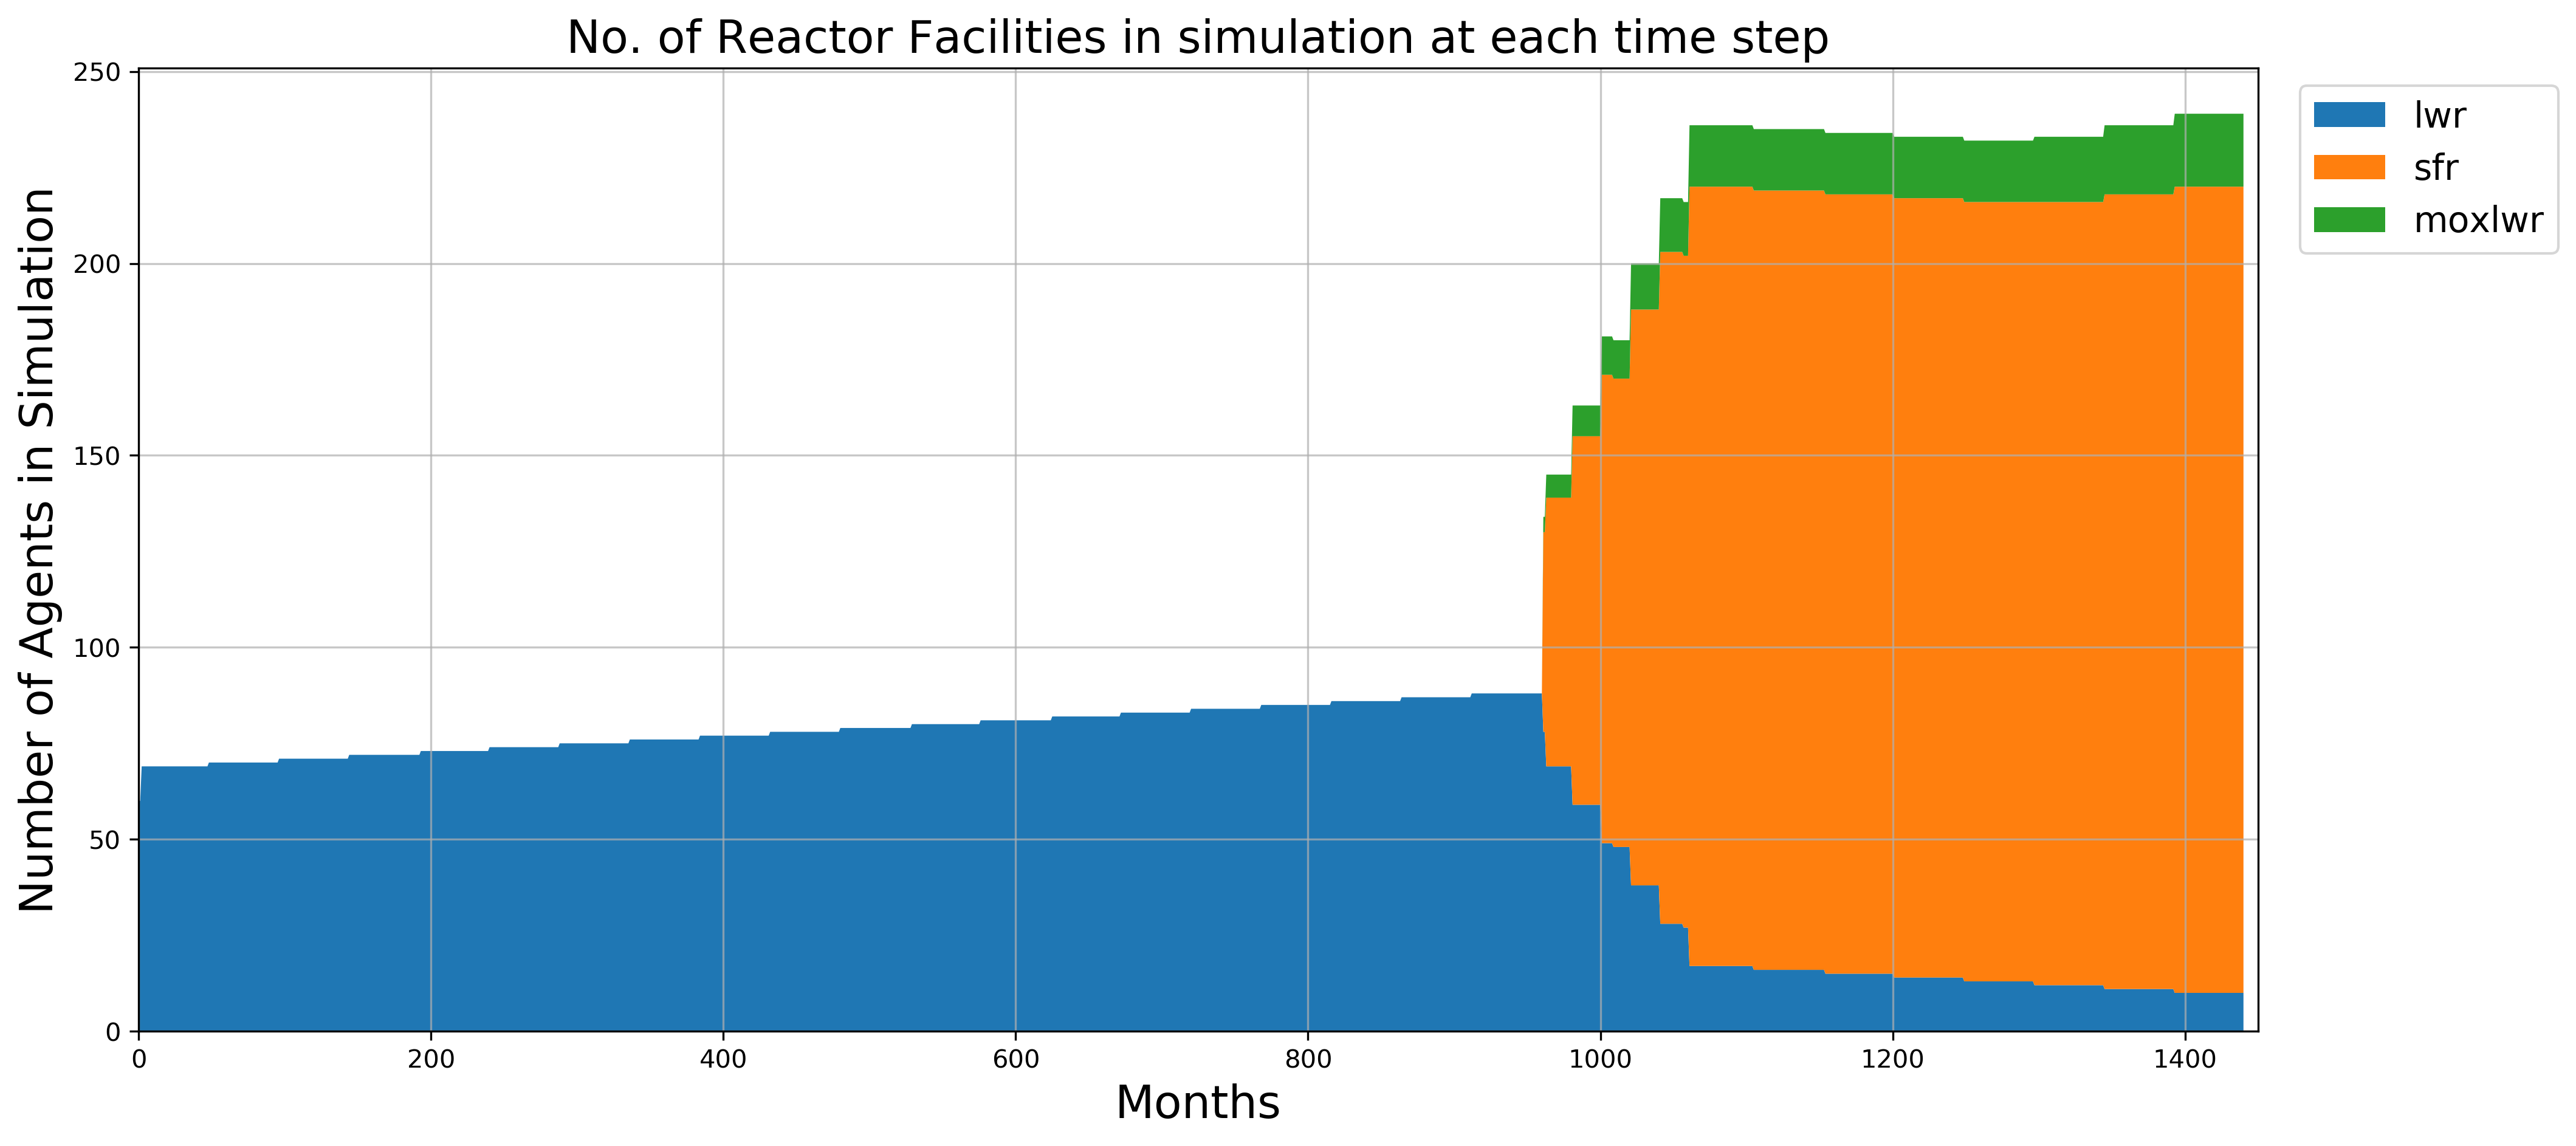
\includegraphics[width=\linewidth]{30-figures/eg30-stack_reactor.png} 
		\caption{EG01-30: Reactor Deployment}
		\label{fig:30reactor}
	\end{subfigure}
	\vspace{1cm}
	\begin{subfigure}[t]{1.2\textwidth}
		\centering
		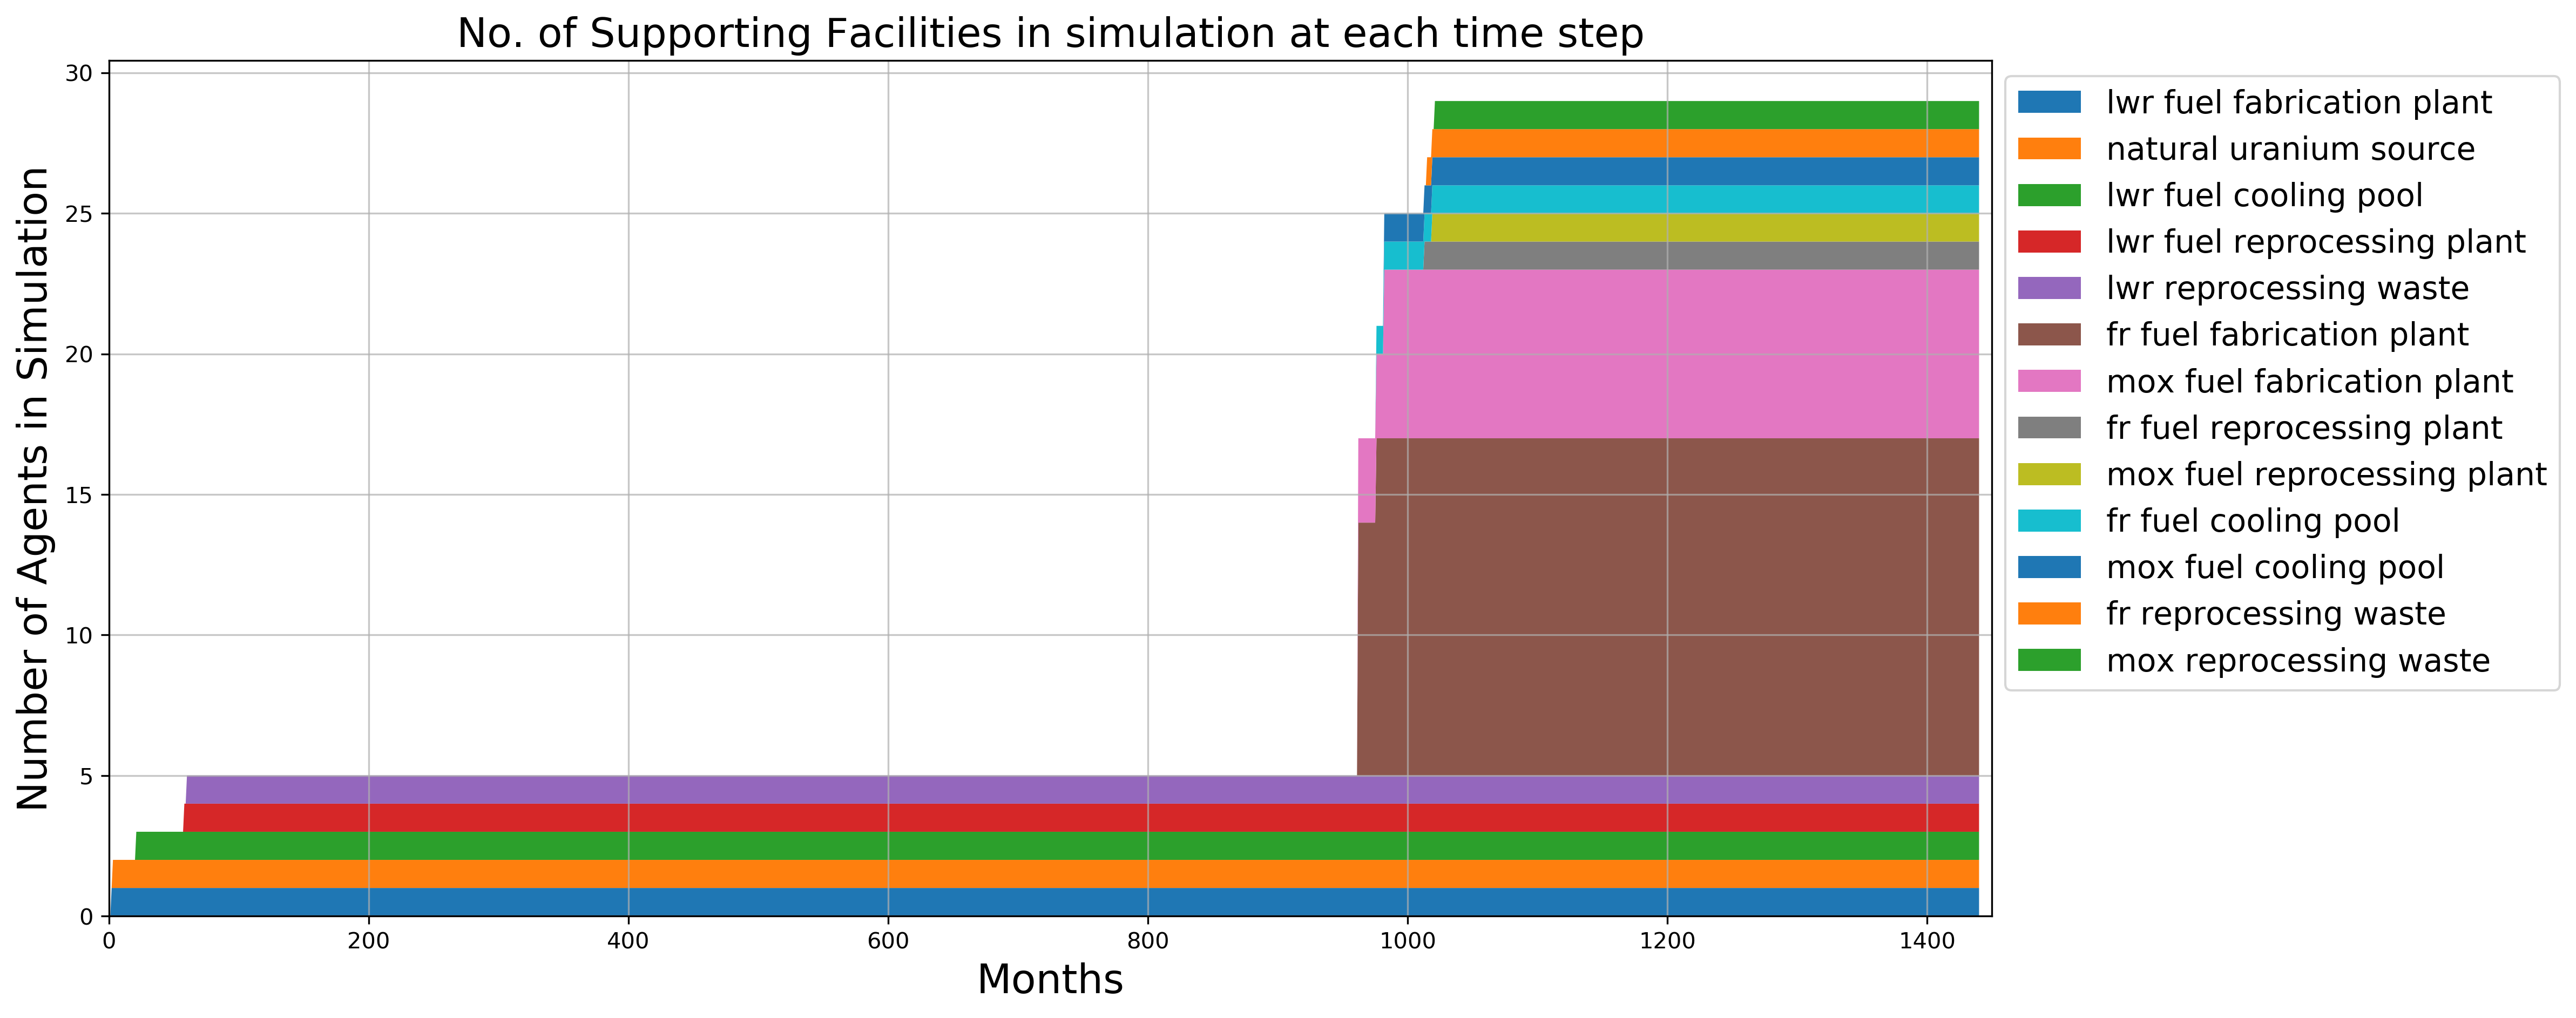
\includegraphics[width=\linewidth]{30-figures/eg30-stack_support.png} 
		\caption{EG01-30: Supporting Facility Deployment}
		\label{fig:30support}
	\end{subfigure}
	\hfill
	\caption{Time dependent deployment of reactor and supporting facilities in 
	the EG01-30 linearly increasing power demand transition scenario. 
	\deploy automatically deploys reactor and supporting facilities 
	to setup a supply chain to meet linearly increasing power demand of $60000 + 250t/12$ MW
	during a transition from \glspl{LWR} to MOX LWRs and \glspl{SFR}. }
	\label{fig:30stack}
\end{figure}

\pagebreak
\bibliography{2019-ddca}

\end{document}
